\documentclass[10pt, aspectratio=169, unknownkeysallowed]{beamer} 
%--------------------------------------TEMA DE LA PRESENTACI�N---------------------------------------%
\mode<presentation>
{
  \usetheme{Warsaw}
  \setbeamercovered{invisible}%dynamic
  \setbeamertemplate{blocks}[rounded][shadow=true]
  \setbeamertemplate{navigation symbols}{}%eliminar botones de navegacion
  \hypersetup{pdfpagemode=FullScreen} %Comentar para que no se abra automaticamente pantalla completa
}%------------------------------------------PAQUETES-------------------------------------------------------%
\usepackage{mispaquetes}
%----------------------------------------DEFINICIONES----------------------------------------------------%
\usepackage{misdefiniciones}
\usepackage{mititulo}
%-----------------COLORES------------------%
\usepackage{miscolores}

%%%%%%%%%%%%%%%%%%%%%%%%%%%%%%%%%%%%%%%%%%%%%%%%%%%%
%-----------------------------------------------DOCUMENTO----------------------------------------------------------%
%%%%%%%%%%%%%%%%%%%%%%%%%%%%%%%%%%%%%%%%%%%%%%%%%%%%


%\includeonly{Secciones/Seccion9_Conclusion}
\begin{document}
%--------------T�tulo----------------%
\begin{frame}
  \titlepage
\end{frame}
%--------------�ndice----------------%\
\begin{frame}{�ndice general}
\begin{multicols}{2}
  \setcounter{tocdepth}{1}  
  \tableofcontents
\end{multicols}
\end{frame}

%-----------------------------------------------SECCIONES----------------------------------------------------------%

\section{Introducci�n}
\subsection{�Qu� es esto del \LaTeX?}

\begin{frame}[t]{Un procesador de textos: Del \TeX{} al \LaTeX{}}%[plain] para que ocupe toda la pantalla
\begin{block}{El \TeX{}}
\begin{itemize}
\item \pause Creado por Donald E. Knuth (Univ. de Stanford)
\item \pause Proviene de la palabra {\em technology}, cuya ra�z griega es $\tau\epsilon\chi\equiv$ {\em arte}
\item \pause Como todo lenguaje de programaci�n:
\begin{itemize}
\item Gran {\color{miverdeO}potencia} y {\color{miverdeO}flexibilidad}
\item {\color{red}Complejidad} para aquellos no familiarizados con la programaci�n
\end{itemize}
\end{itemize}
\end{block}

\begin{block}{El \LaTeX}
\begin{itemize}
\item \pause Leslie Lamport ({\em Digital Equipment Corp.})
\item \pause Conjunto de {\bf �rdenes} que acercan el \TeX{} a los mortales
\item \pause Se normaliza el \LaTeX{}: \LaTeX$2_\varepsilon$
\end{itemize}
\end{block}
\end{frame}

\subsection{�Por qu� utilizarlo?}

\begin{frame}{�Por qu� utilizarlo?}
\begin{multicols}{2}
\begin{itemize}
\item \pause Es software libre
\item \pause Funciona sobre casi cualquier tipo de sistema y arquitectura (incluso las gratuitas)
\item \pause {\color{red}Auto}enumera las f�rmulas y ecuaciones
\item \pause Crea �ndices de contenido, tablas, figuras y de t�rminos �{\color{red}auto}m�ticamente!
\item \pause Permite el uso de Bib\TeX{}
\item \pause Resultado profesional
\item \pause Buen soporte para las matem�ticas
\item \pause Para que las cosas queden monas ya est�n otros: {\color{red}\LaTeX{} lo hace por t�}
\item \pause Los archivos ocupan muy poco
\end{itemize}
\end{multicols}
\end{frame}

\begin{frame}{Dos filosof�as a la hora de procesar documentos}
\begin{columns}
\column{0.5\textwidth}
\pause\begin{defi}{WYSIWYG}
Acr�nimo de {\em What You See Is What You Get}
\end{defi}
\begin{ejem}{WYSIWYG}
\begin{itemize}
\item Word
\item Google Docs 
\item Wordpress
\item Open Office 
\item \ldots
\end{itemize}
\end{ejem}
\column{0.51\textwidth}
\pause\begin{defi}{WYSIWYM}
Acr�nimo de {\em What You See Is What You Mean}
\end{defi}
\begin{ejem}{WYSIWYM}
\vspace{0.8cm}
\centering
\invisible<1-3>{\Huge�\LaTeX{}!}
\pause\vspace{0.8cm}
\end{ejem}
\vfill
\end{columns}
\end{frame}

\subsection{�Merece la pena?}
\begin{frame}{Los inconvenientes\ldots �son inconvenientes?}
\begin{columns}[T]
\column[T]{0.7\textwidth}
\vspace{-2.5cm}
\uncover<1->{Los inconvenientes que la gente suele remarcar son:}
\begin{itemize}
\item <2->\alert<6>{\em ``Me frustra mucho la complejidad, �por qu� hacerlo tan dif�cil?''.}
\item <3->\alert<7>{\em  ``Tardo mucho en escribir un simple art�culo.''.}
\item <4->\alert<8>{\em ``Esto tambi�n lo hace Word''.}
\end{itemize}

\uncover<5->{Preg�ntate:}
\begin{itemize}
\item <6-> \alert<6>{�Cu�ntas palabras sabes entre el castellano y el ingl�s? �Qu� suponen algunas decenas m�s?}
\item <7-> \alert<7>{ �Cu�nto tardar�as en escribir algo en Word con la misma calidad?}
\item <8-> \alert<8>{�No est�s harto de coger el rat�n para insertar las f�rmulas? �No te gustar�a que los �ndices y las referencias se hicieran solos,  y los elementos flotantes no se comieran el texto?}
\end{itemize}
\column[c]{0.3\textwidth}
\vspace{0.5cm}

\begin{figure}
\centering
\begin{tikzpicture}
\alt<6->{\node[opacity=1]{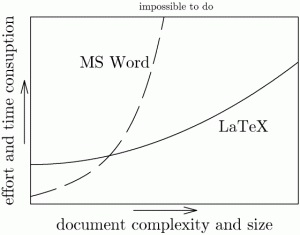
\includegraphics[width=\textwidth]{Figuras/CurvaAprendizaje2.jpg}};}
{\node[opacity=0.01]{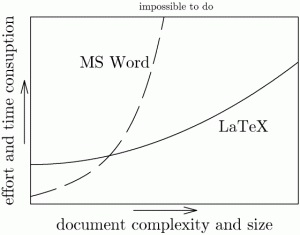
\includegraphics[width=\textwidth]{Figuras/CurvaAprendizaje2.jpg}};}
\end{tikzpicture}
\vspace{-0.75cm}
\uncover<6->{\caption{Coste {\em vs.} complejidad para \LaTeX{} y Word}}
\label{fig:CurvaAprendizaje}
\end{figure}
\end{columns}
\end{frame}

\subsection*{�nimo}
\section{�C�mo empiezo?}

\subsection{Modo de funcionamiento}

\begin{frame}{El funcionamiento de \LaTeX{}}
\begin{enumerate}
\item <1-> \alert<1>{Escribir el contenido \textbf<1>{estructurado} mediante el \textbf<1>{lenguaje} marcado}
\item <2-> \alert<2>{Se \textbf<2>{compila}, y \LaTeX{} se encarga de \textbf<2>{dar formato} al texto}
\item <3-> \alert<3>{\textbf<3>{Visualizaci�n} por pantalla del fichero resultante}
\end{enumerate}
\only<4->{
\begin{figure}[hbtp]
\centering
\begin{tikzpicture}
\alt<4->{\node[opacity=1]{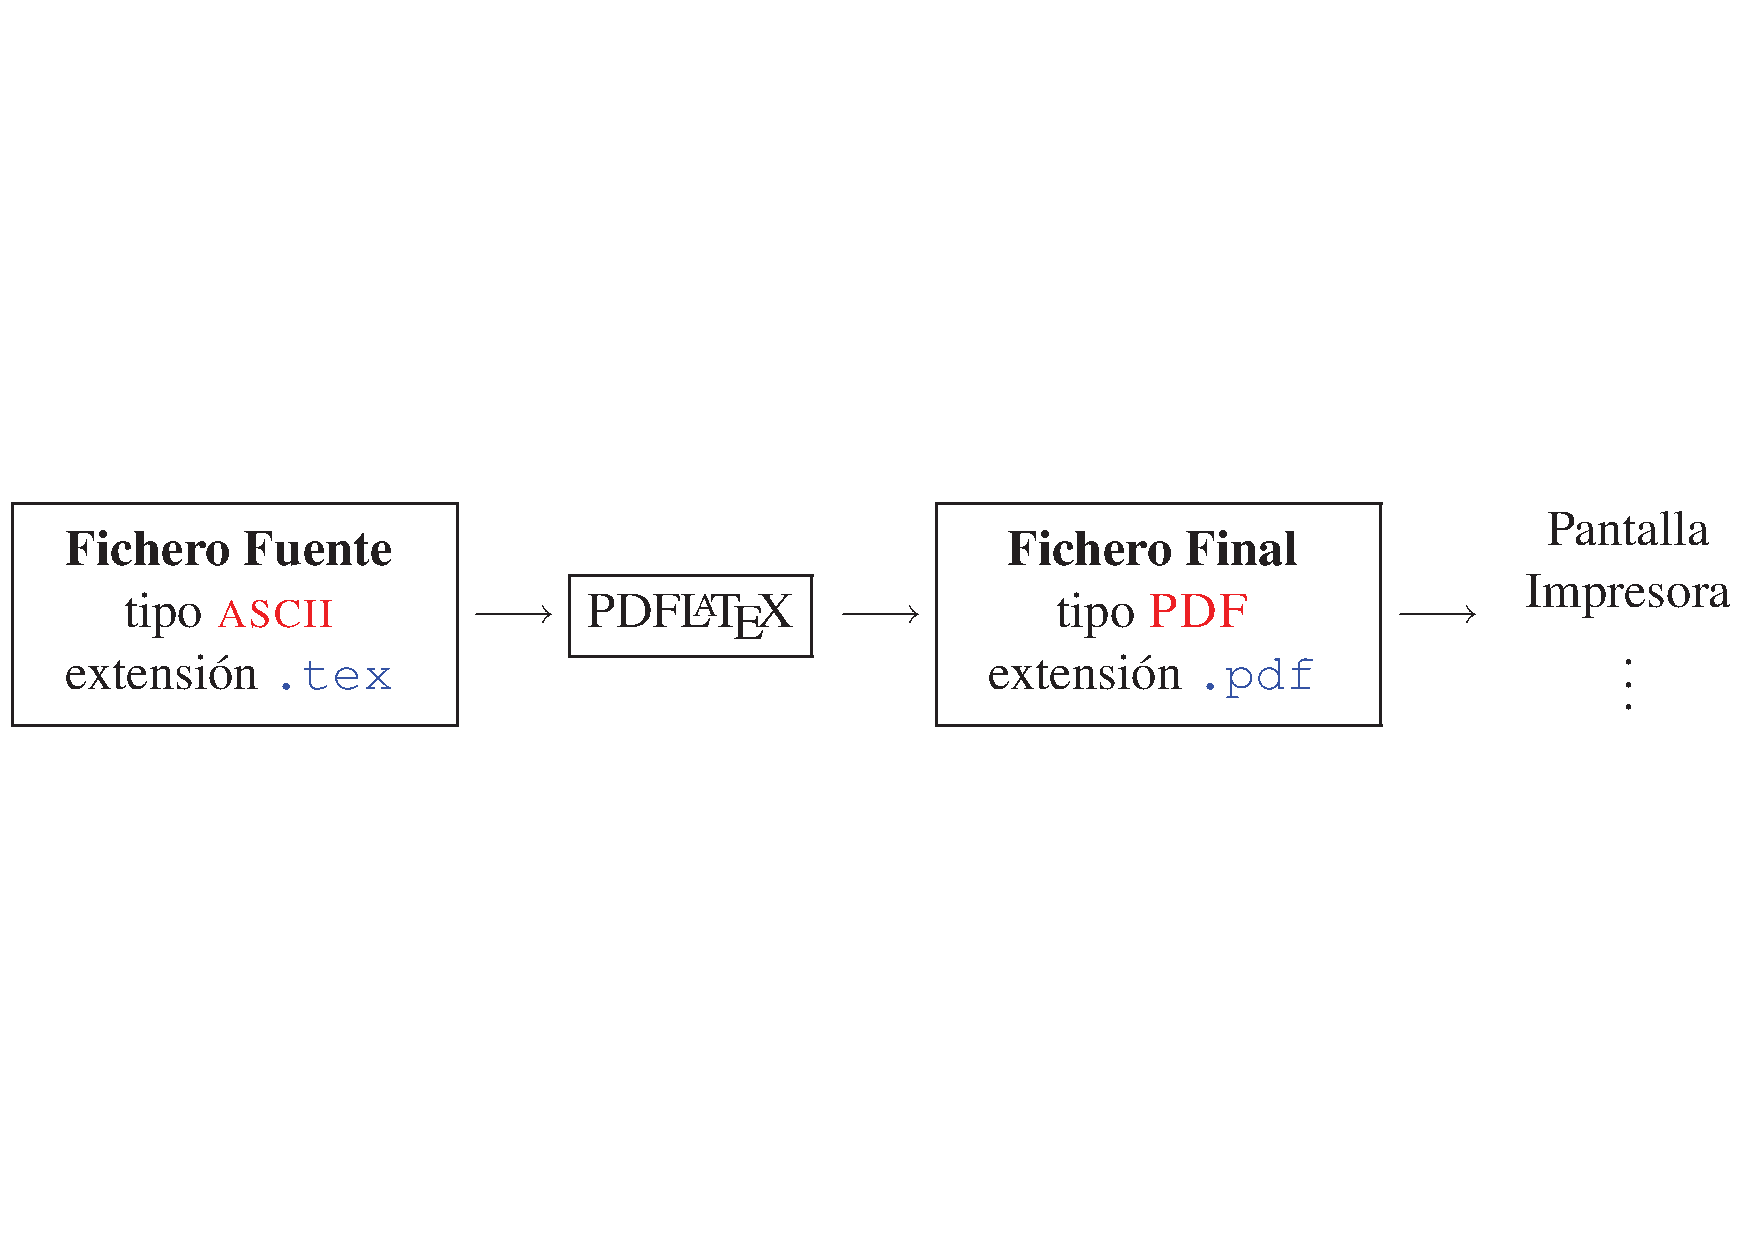
\includegraphics[width=\textwidth]{Figuras/funcionamiento}};}
{\node[opacity=0.01]{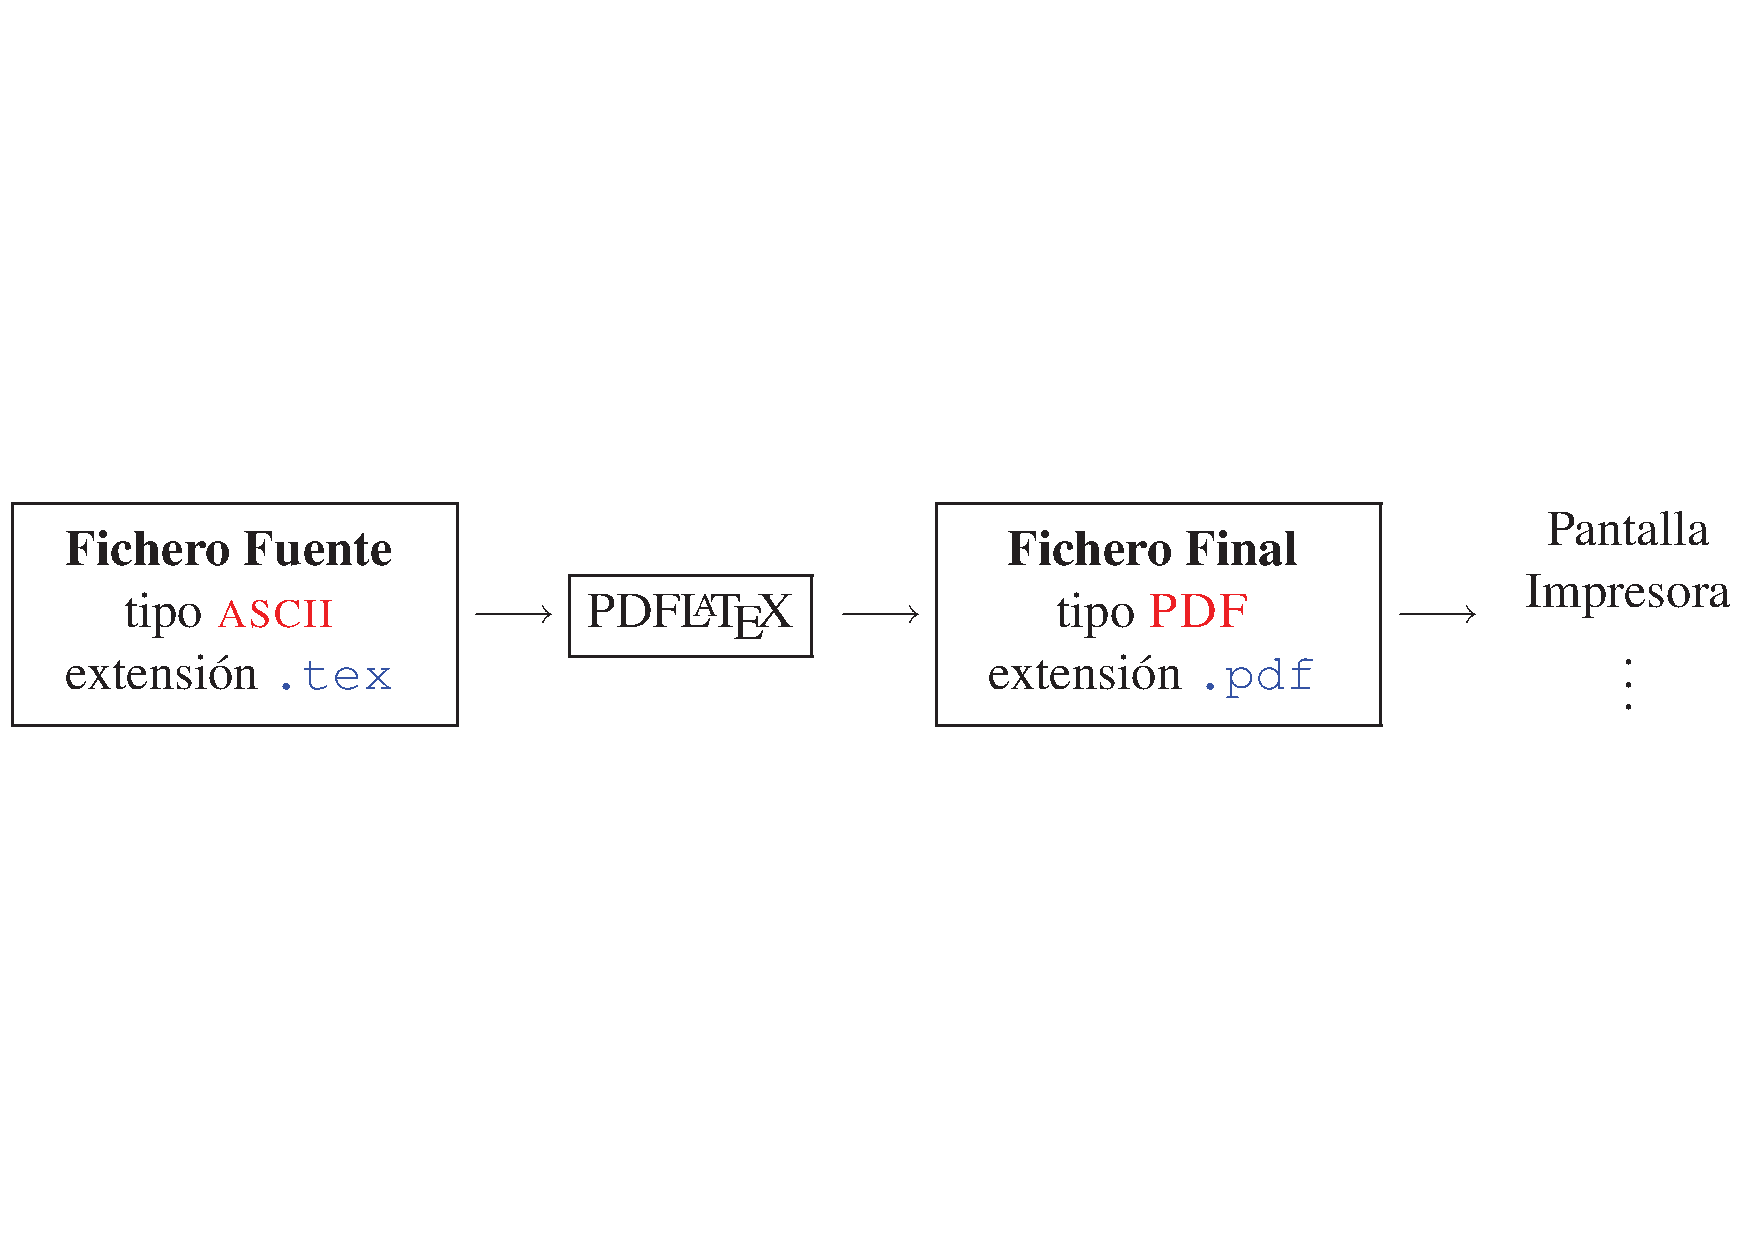
\includegraphics[width=\textwidth]{Figuras/funcionamiento}};}
\end{tikzpicture}
\vspace{-0.75cm}
\visible<4->{\caption{Modo de funcionamiento de \LaTeX{} (PDF\LaTeX{})}}
\label{fig:CurvaAprendizaje}
\end{figure}}
\end{frame}

\subsection{Los requerimientos}
\begin{frame}{Los  requerimientos}
Necesitaremos tener instalado en nuestro ordenador:
\begin{itemize}
\item<2-> \alert<2>{Acrobar Reader}
\item<3-> \alert<3>{Una distribuci�n de \TeX{} y \LaTeX{}:}
\visible<4->{\begin{itemize}
\item Para Windows: MiK\TeX
\item Para Linux/Unix: te\TeX
\item Para MacOSX: \TeX Shop
\end{itemize} }
\end{itemize}
\visible<5->{Cualquiera de estas distribuciones posee:}
\visible<6->{
\begin{itemize}
\item<6->  \alert<6>{Ventana de editor}
\item<7-> \alert<7>{Ventana de compilaci�n (para visualizar pasos, errores y precauciones (\textbf<8>{\em warnings}))}
\item<8-> \alert<8>{Ventana de visualizaci�n del fichero generado}
\end{itemize}}
\end{frame}
\section{El documento}

%----------------------------------------%----------------------------------------%----------------------------------------
\subsection{Un ejemplo}
\begin{frame}[fragile]{Una carta formal}
\vspace{-0.7cm}
\begin{columns}
\column{0.5\textwidth}
\begin{lstlisting}
\documentclass[11pt]{letter} 
\usepackage[latin1]{inputenc}
\usepackage[spanish]{babel}
\usepackage{marvosym}
\begin{document}% Aqu� empieza el documento
\begin{letter}{D�a. M�nica {\it Limonero Guti�rrez}. Subdirectora de Relaciones Internacionales\\
{\sc Oficina Informaci�n Internacional}:\\
Direcci�n y Adjunt�a para Movilidad y Extensi�n Internacional \\
EMPRESA. Calle Sinesio Gordito. \\
280XX MADRID,  ESPA�A} 
\begin{center}% Este entorno centra lo que incluye
\large\bf Perico del Dedo Delgado \\
Calle del Hambre, 5, piso 1, puerta A\\ Ja�n, Espa�a \\ +34 600 00 00 XX\\ 
pededo\MVAt delgado.com
\end{center} 
\signature{Perico del Dedo Delgado}
\opening{Estimada Sra. Limonero,} 
Lorem ipsum % Texto modelo
A la espera de una respuesta, quedo a su entera disposici�n para facilitarles cualquier informaci�n complementaria.
\closing{Reciban un cordial saludo, }
\encl{Documentos que puedan ser de su inter�s} 
\end{letter}
\end{document}
\end{lstlisting}


\column{0.5\textwidth}

\begin{figure}
\centering
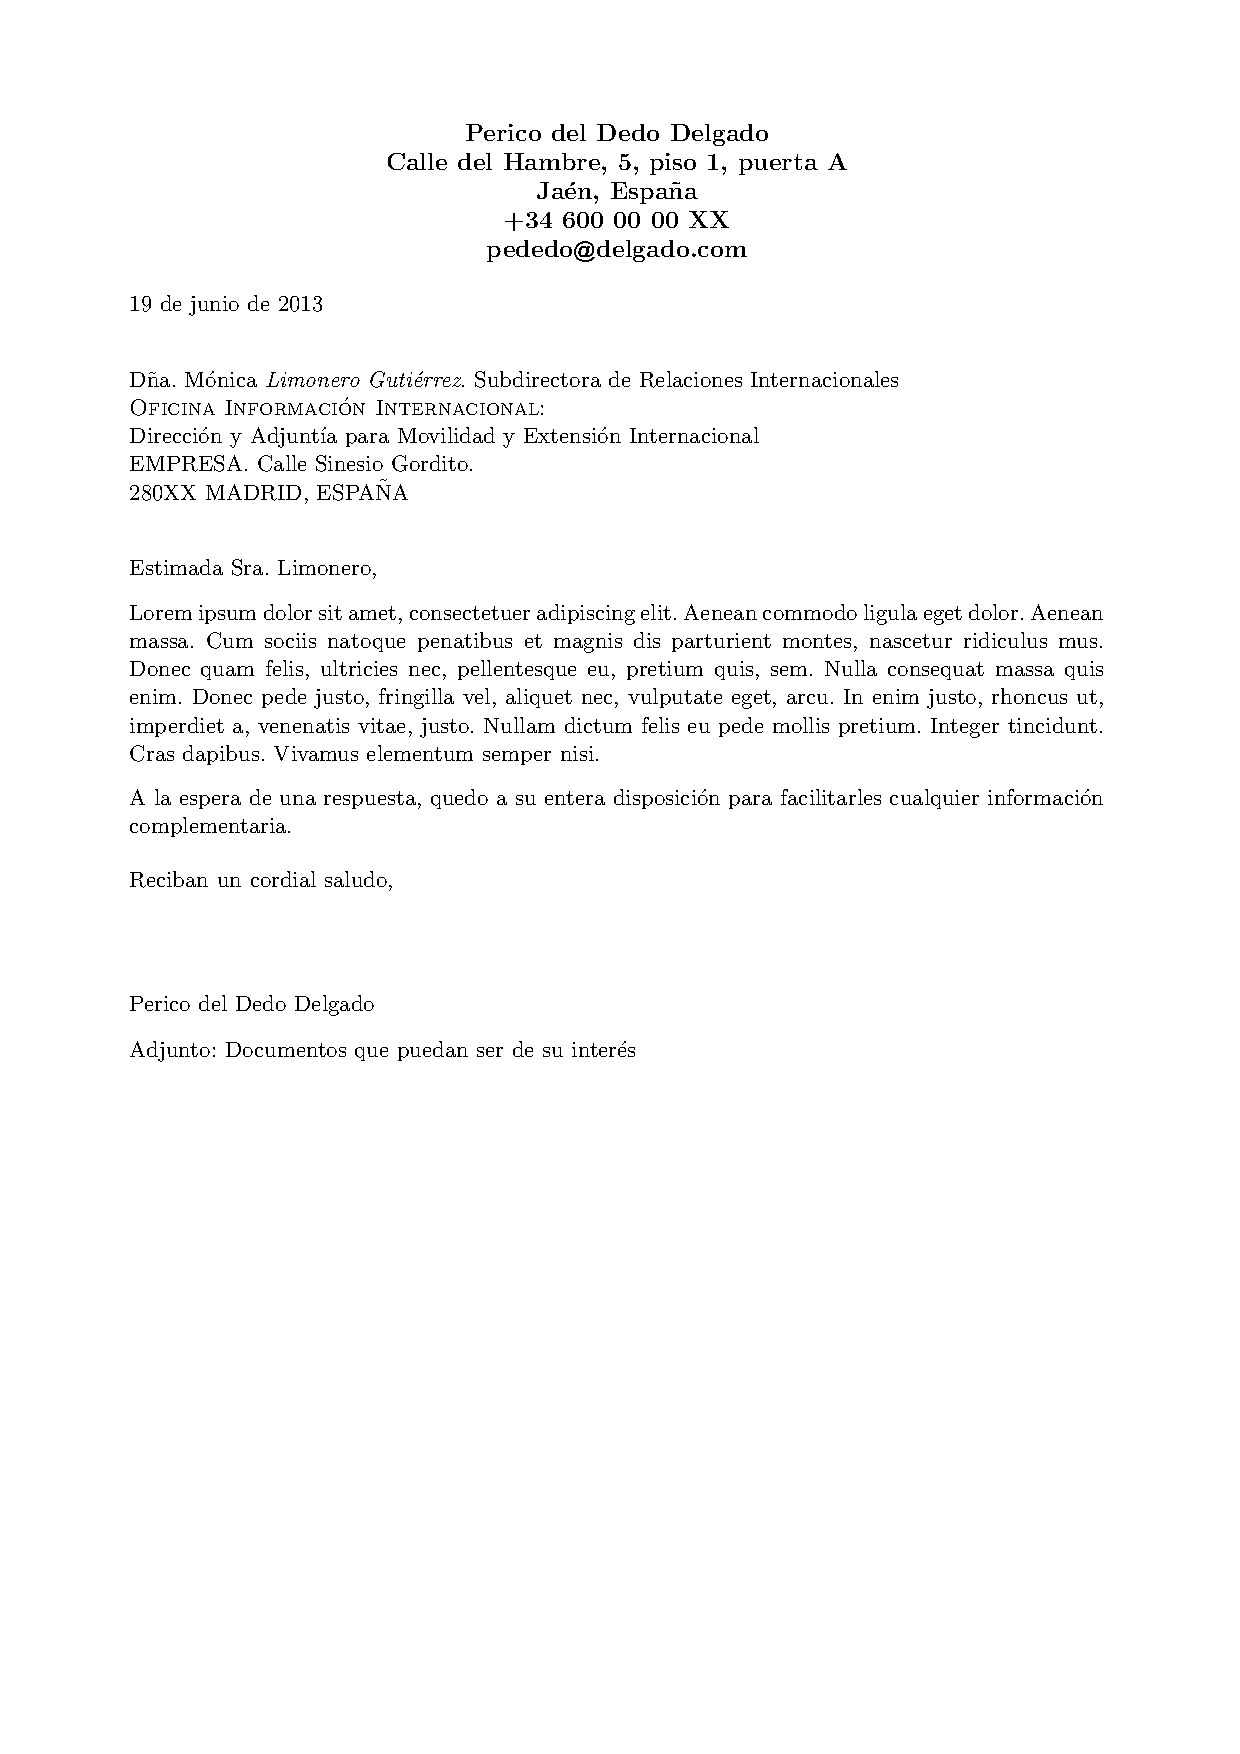
\includegraphics[width=\textwidth]{FigurasEjemplos/CartaREC.pdf}
\label{fig:EjemploCarta}
\end{figure}
\end{columns}
\end{frame}


%----------------------------------------%----------------------------------------%----------------------------------------
\subsection{El fichero fuente}

\begin{frame}{El fichero fuente: el editor}
\pause Encontramos dos partes bien diferenciadas:
\pause
\begin{center}
\begin{tabular}{rl}
Pre�mbulo
&
$\left\{ \begin{array}{l}
	\mbox{\texttt{\textbackslash  documentclass[<{\em opciones}>]\{<clase>\}}}\\
	\mbox{\texttt{\textbackslash usepackage[<{\em opciones}>]\{<paquete>\}}}\\
	\mbox{\vdots}\\
	\mbox{\texttt{\textbackslash usepackage[<{\em opciones}>]\{<paquete>\}}}\\
	\mbox{\texttt{\% Macros}}\\
	\end{array} \right. $
\par\\
\\
Cuerpo
&
$\left\{ \begin{array}{l}
	\mbox{\texttt{\textbackslash begin\{document\}}}\\
	\mbox{\texttt{\hspace{1cm}\textbackslash section\{}La comida\texttt{\}}}\\
	\mbox{\texttt{\hspace{1cm}\textbackslash subsection\{}La fruta\texttt{\}}}\\
	\mbox{\texttt{\hspace{1cm}\textbackslash subsubsection\{}Las manzanas\texttt{\}}}\\
	\mbox{\texttt{\textbackslash end\{document\}}}
	\end{array} \right. $
\end{tabular}
\end{center}
\end{frame}
%----------------------------------------%----------------------------------------%----------------------------------------
\subsection{El pre�mbulo}

\begin{frame}{Definici�n del documento: las opciones (I)}
\pause
Es la primera l�nea de c�digo que escribiremos. Aqu� se localizar�n las caracter�sticas del documento, tama�o de papel, tipo de documento, \ldots
\pause 
\begin{sintax}{\texttt{\textbackslash documentclass}}
\texttt{\textbackslash documentclass[<{\em opciones}>]\{<clase>\}}
\end{sintax}

\pause
\begin{ejem}{\texttt{\textbackslash documentclass}}
\texttt{\textbackslash documentclass[10pt, a4paper, landscape, openright]\{book\}}
\texttt{\textbackslash documentclass[10pt, a4paper]\{article\}}
\end{ejem}
\pause
Las opciones son:
\begin{multicols}{3}
\begin{itemize}
\item Tama�o de la fuente
\item Tama�o y formato del papel
\item Estilo multicolumna
\item Estilo de numeraci�n de las ecuaciones
\item Modo apaisado
\item P�gina de apertura de cap�tulo
\item P�gina para portada
\item Impresi�n a dos caras
\end{itemize}
\end{multicols}
\end{frame}

\begin{frame}{Definici�n del documento: las opciones (II)}
\pause
\begin{acla}{Tama�o de letra}
Valores posibles: \texttt{10pt (default), 11pt, 12pt}.
Suficiente para casi cualquier tipo de documento.
\texttt{\textbackslash usepackage\{extsizes\}} amplia la gama.
\end{acla}

\pause
\begin{acla}{Tama�o y formato del papel}
Valores posibles: \texttt{a4paper (default), letterpaper, a5paper, b5paper, executivepaper, legalpaper}.
\texttt{\textbackslash usepackage\{geometry\}} amplia los tipos.
\end{acla}

\pause
\begin{acla}{Borrador o definitivo}
Valores posibles: \texttt{draft, final}.
\end{acla}

\pause
\begin{acla}{Columnas}
Valores posibles: \texttt{onecolumn (default), multicolumn}.
\texttt{\textbackslash usepackage\{multicols\}} amplia las posibilidades.
\end{acla}
\end{frame}
\begin{frame}{Definici�n del documento: las opciones (III)}
\vspace{-0.18cm}
\pause
\begin{acla}{Ecuaciones}
Valores posibles (indep.): \texttt{fleqn} (alineados a la izq.), \texttt{leqno} (etiquetas a la izq.).
\end{acla}

\pause
\begin{acla}{Vertical o apaisado}
Valores posibles: \texttt{landscape} (apaisado). Su omisi�n implica formato vertical.
\end{acla}

\pause
\begin{acla}{Doble cara}
Valores posibles: \texttt{oneside} (defalut en {\em article} y {\em report}), \texttt{twosides} (default en {\em book}).
\end{acla}

\pause
\begin{acla}{Portada}
Valores posibles: \texttt{notitlepage} (defalut en {\em article}), \texttt{titlepage} (default en {\em book}  y en {\em report}).
\end{acla}

\pause
\begin{acla}{Apertura de cap�tulos}
Valores posibles: \texttt{openany} (defalut en {\em report}), \texttt{openright} (default en {\em book}). {\em article} {\color{red}NO soporta el comando \texttt{\textbackslash chapter}}
\end{acla}
\end{frame}

\begin{frame}{Los paquetes}
\begin{itemize}
\item \pause Son los equivalentes a las librer�as de \texttt{C} o \texttt{C++}.
\item \pause Existen much�simos, y muchos de ellas {\color{red} muy pr�cticos}.
\item \pause Tambi�n puedes crear tu propia librer�a o {\em archivo de estilo (\texttt{.sty})}.
\end{itemize}
\pause 
\begin{sintax}{\texttt{\textbackslash usepackage}}
\texttt{\textbackslash usepackage[<{\em opciones}>]\{<nombre del paquete>\}}
\end{sintax}

\pause
\begin{ejem}{\texttt{\textbackslash usepackage}}
\texttt{\textbackslash usepackage[framed,autolinebreaks,useliterate]\{mcode\}}
\texttt{\textbackslash usepackage[latin1]\{inputenc\}}
\end{ejem}
\pause
\begin{itemize}
\item \pause Aqu� las opciones dependen del paquete en concreto.
\item \pause De forma general, habr� que instalarlos (con MiK\TeX{} ir a \textbf{Inicio$\rightarrow$Todos los programas$\rightarrow$MikTeX$\rightarrow$Maintenance (admin)$\rightarrow$Package Manager (Admin)}).
\end{itemize}
\end{frame}

\begin{frame}{Las definiciones (o macros)}
\begin{itemize}
\item \pause Sirven para ense�ar a \LaTeX{} c�mo escribir lo que queramos, como queramos y de forma c�moda.
\item \pause B�sicamente se distinguen dos:
\begin{itemize}
\item \pause Los comandos (\texttt{\textbackslash newcommand} y \texttt{\textbackslash renewcommand}).
\item \pause Los entornos (\texttt{\textbackslash newenvironment}).
\end{itemize}
\end{itemize}
\pause 
\begin{sintax}{\texttt{\textbackslash newcommand}}
\texttt{\textbackslash newcommand\{<{\em nombre comando}>\}[<{\em n�mero}>]\{<{\em definici�n}>\}}
\end{sintax}
\pause
\begin{sintax}{\texttt{\textbackslash renewcommand}}
\texttt{\textbackslash renewcommand\{<{\em comando}>\}[<{\em n�mero}>]\{<{\em redefinici�n}>\}}
\end{sintax}
\pause
\begin{sintax}{\texttt{\textbackslash newenvironement}}
\texttt{\textbackslash newenvironment\{<{\em nombre}>\}[<{\em n�mero}>]\{<{\em antes}>\}\{<{\em despu�s}>\}}
\end{sintax}

\end{frame}




%newcommand
\begin{frame}[fragile]{\small \texttt{\textbackslash newcommand\{<{\em nombre comando}>\}[<{\em n�mero}>]\{<{\em definici�n}>\}}}
\begin{itemize}
\item \pause \texttt{\em nombre comando}: Es el c�digo con el que se va a escribir lo que queramos, por ejemplo \texttt{\textbackslash LaTeX} da lugar a \LaTeX.
\item \pause \texttt{\em n�mero}: n�mero de argumentos que recibe el comando.
\item \pause\texttt{\em definici�n}: Aqu� se pone lo que se tiene que hacer al escribir el comando.
\end{itemize}
\pause
\begin{ejem}{\texttt{\textbackslash newcommand}}

\begin{columns}
\column{0.4\textwidth}

\begin{lstlisting}
\newcommand{\micomando}[1] {
 Este ejemplo en  \LaTeX{} trata de #1}

% EN EL CUERPO DEL DOCUMENTO:
\begin{itemize}
\item \micomando{comandos}.
\end{itemize}
\end{lstlisting}
\column{0.49\textwidth}
\begin{itemize}
\item Este ejemplo en  \LaTeX{} trata de comandos.
\end{itemize}
\end{columns}
\end{ejem}
\end{frame}

% renewcommand
\begin{frame}[fragile]{\small \texttt{\textbackslash renewcommand\{<{\em nombre comando}>\}[<{\em n�mero}>]\{<{\em redefinici�n}>\}}}
\begin{itemize}
\item \pause \texttt{\em nombre comando}: Es el nuevo c�digo con el que nos referiremos a un c�digo antiguo.
\item \pause \texttt{\em n�mero}: n�mero de argumentos que recibe el comando.
\item \pause\texttt{\em redefinici�n}: Aqu� se pone lo que se quiere  hacer al escribir el comando, en lugar de lo que se ven�a haciendo hasta ahora.
\end{itemize}
\pause
\begin{ejem}{\texttt{\textbackslash renewcommand}}

\begin{columns}
\column{0.4\textwidth}
\begin{lstlisting}
\renewcommand{\labelitemi}{$\star$}
% EN EL CUERPO DEL DOCUMENTO:
\begin{itemize}
\item Punto uno.
\item Punto dos.
\end{itemize}
\end{lstlisting}

\column{0.49\textwidth}
{\bf Antes:}
\begin{itemize}
\item Punto uno.
\item Punto dos.
\end{itemize}

{\bf Despu�s:}
\begin{itemize}
\item [$\star$] Punto uno.
\item [$\star$] Punto dos.
\end{itemize}

\end{columns}
\end{ejem}
\end{frame}

% newenvironment
\begin{frame}[fragile]{\small \texttt{\textbackslash newenvironment\{<{\em nombre}>\}[<{\em n�mero args.}>]\{<{\em antes}>\}\{<{\em despu�s}>\}}}
\begin{itemize}
\item \pause \texttt{\em nombre}: Es el nombre del entorno.
\item \pause \texttt{\em n�mero args.}: n�mero de argumentos que recibe el entorno.
\item \pause\texttt{\em antes}: Lo que se ejecuta antes de compilar el entorno.
\item \pause \texttt{\em despu�s}: Lo 	que se ejecuta al salir del entorno.
\end{itemize}
\pause
\begin{ejem}{\texttt{\textbackslash newenvironment}}

\begin{columns}
\column{0.4\textwidth}
\begin{lstlisting}
\newenvironment{cita}[1]		%recibe un argumento, para el autor
{\begin{quote}\itshape}		% definici�n de la entrada al entorno
{\end{quote}\centerline{#1}}	% salida del entorno
% EN EL CUERPO DEL DOCUMENTO:
\begin{cita}{Confucio}
La ignorancia es la noche de la mente: pero una noche sin luna y sin estrellas.
\end{cita}
\end{lstlisting}

\column{0.49\textwidth}
\begin{quote}
{\it La ignorancia es la noche de la mente: pero una noche sin luna y sin estrellas.}
\end{quote}
\centerline{Confucio}

\end{columns}
\end{ejem}
\end{frame}
%----------------------------------------%----------------------------------------%----------------------------------------
\subsection{El cuerpo}

\begin{frame}{�rdenes y declaraciones}
\begin{itemize}
\item \pause Todo aquello comprendido entre \texttt{\backS begin\{document\}} y \texttt{\backS end\{document\}} es el cuerpo del documento.
\item \pause El cuerpo se constituye por:
\begin{itemize}
\item Texto
\item Instrucciones propias (palabras clave de \LaTeX{})
\end{itemize}
\item \pause Las \alert{instrucciones} propias tienen un \alert{efecto local}
\end{itemize}

\begin{defi}{�rdenes y declaraciones}
Llamaremos {\color{miverdeO}�rdenes} y {\color{miverdeO}declaraciones} a aquellas instrucciones que tienen efecto sobre el texto, como por ejemplo los {\it grupos}, los {\it comandos} y los {\it entornos}.
\end{defi}
\end{frame}

\begin{frame}[fragile]{Los grupos}
\begin{itemize}
\item \pause Son cualquier \alert{parte} del documento \alert{DELIMITADA}.
\item \pause Limitadores:
\begin{itemize}
\item Llaves (\texttt{\{} y \texttt{\}})
\item Inicio y final de entorno (\texttt{\backS begin\{<{\it nombre del entorno}>\}} y \texttt{\backS end\{<{\it nombre del entorno}>\}})
\end{itemize}
\end{itemize}
\pause
\begin{ejem}{Grupo delimitado por entorno (\texttt{itemize}) y llaves}

\begin{columns}[c]

\column{0.45\textwidth}
\begin{lstlisting}
\begin{itemize}
\item  Me gustan las manzanas de color {\color{red} rojo}.
\item  Pues a mi los textos en {\bf negrita} y en {\it it�lica}.
\end{itemize}
\end{lstlisting}

\column{0.45\textwidth}
\begin{itemize}
\item  Me gustan las manzanas de color {\color{red} rojo}.
\item  Pues a mi los textos en {\bf negrita} y en {\it it�lica}.
\end{itemize}

\end{columns}
\end{ejem}

\end{frame}

\begin{frame}[fragile]{Los comandos}
\begin{itemize}
\item \pause Son \alert{�rdenes sencillas} que comienzan con una \texttt{\alert{\backS}}, seguida de uno o varios caracteres.
\item \pause Adem�s, est�n los diez caracteres reservados de \TeX{}:
\end{itemize}
\pause
\begin{acla}{Los 10 caracteres reservados}
\hfill\texttt{\%}
\hfill\texttt{\backS}
\hfill\texttt{\{}
\hfill\texttt{\}}
\hfill\texttt{\&}
\hfill\texttt{\~{}}
\hfill\texttt{\$}
\hfill\texttt{\_}
\hfill\texttt{\^{}}
\hfill\texttt{\#}
\end{acla}
\pause
\begin{sintax}{Comandos}
\texttt{\backS comando[<{\em args. optativos}>]\{>{\em args. obligatorios}>\}}
\end{sintax}
\pause
\begin{ejem}{Algunos comandos}
\texttt{\backS section[Verduras]\{Las verduras\}} crea una secci�n de t�tulo ``Las verduras'' y en la TOC aparece como ``Verduras''.

\texttt{\backS texttt\{texto\}} permite excribir en formato m�quina de escribir: \texttt{texto}.

\texttt{\backS textregistered} produce \textregistered.
\end{ejem}

\end{frame}

\begin{frame}[fragile]{Los entornos}
\begin{itemize}
\item \pause Son \alert{grupos} que gestionan qu� hacer al \alert{entrar} y al \alert{salir} de ellos.
\item \pause Su contenido (argumentos) puede ser muy extenso.
\end{itemize}

\begin{sintax}{Entornos}
\texttt{\backS begin\{nom. entorno\}[<{\em args. optativos}>]\{<{\em args. obligatorios}>\}}

{\em Objeto o cuerpo del entorno}

\texttt{\backS end\{nom. entorno\}}
\end{sintax}
\begin{ejem}{Entorno para justificar a la derecha}
\begin{columns}[c]

\column{0.45\textwidth}
\begin{lstlisting}
\begin{flushright}
Este es un texto justificado \\% cambio de l�nea
a la derecha
\end{flushright}
\end{lstlisting}

\column{0.45\textwidth}
\begin{flushright}
Este es un texto justificado \\% cambio de l�nea
a la derecha
\end{flushright}
\end{columns}
\end{ejem}
\end{frame}

%----------------------------------------%----------------------------------------%----------------------------------------

\begin{frame}{Recapitulaci�n}
\pause Encontramos dos partes bien diferenciadas en el c�digo fuente de un documento:
\begin{center}
\begin{tabular}{rl}
\uncover<2->{Pre�mbulo}
&
\uncover<3->{$\left\{ \begin{array}{l}
	\uncover<4->{\mbox{Clase de documento (\texttt{\backS documentclass})}}\\
	\uncover<5->{\mbox{Paquetes (\texttt{\backS usepackage})}}\\
	\uncover<6->{\mbox{Macros}}\uncover<7->{\left\{ \begin{array}{l}
		\uncover<7->{\mbox{\texttt{\backS newcommand}}}\\
		\uncover<7->{\mbox{\texttt{\backS renewcommand}}}\\
		\uncover<7->{\mbox{\texttt{\backS newenvironment}}}\\
		\end{array} \right. }
	\end{array} \right. $}
\par\\
\\
\uncover<8->{Cuerpo}
&
\uncover<9->{
$\left\{\begin{array}{l}
	\uncover<9->{\mbox{Grupos}}\\
	\uncover<10->{\mbox{Comandos (\texttt{\backS comando})}}\\
	\uncover<11->{\mbox{Entornos (\texttt{\backS begin\{{\em entorno}\}\ldots\backS end\{{\em entorno}\}})}}\\
	\end{array} \right. $}
\end{tabular}
\end{center}
\end{frame}
%----------------------------------------%----------------------------------------%----------------------------------------

%----------------------------------------
\subsection{Clases de documentos}
\begin{frame}[fragile]{Clases de documentos}
\uncover<1->{
\begin{defi}{Art�culo}
Trabajos cortos (10 o 20 p�ginas). Adecuado para publicar en revistas t�cnicas y de investigaci�n.
\only<2>{
\vspace{-0.1cm}
\begin{center}
\begin{minipage}{0.9\textwidth}
\begin{acla}{Opciones por defecto}
\texttt{\backS documentclass[10pt, letterpaper, final, oneside, onecolumn, notitlepage]\{article\}}
\end{acla}
\end{minipage}
\end{center}}
\end{defi}}

\uncover<3->{
\begin{defi}{Report}
Trabajos grandes: tesis, proyectos, apuntes, memorias, narraci�n corta, informes, \ldots
\only<4>{
\begin{center}
\begin{minipage}{0.9\textwidth}
\begin{acla}{Opciones por defecto}
\texttt{\backS documentclass[10pt, letterpaper, final, oneside, openany, onecolumn, titlepage]\{article\}}
\end{acla}
\end{minipage}
\end{center}}
\end{defi}}

\uncover<5->{
\begin{defi}{Book}
Trabajos muy grandes. Destinado a libros y documentos susceptibles de publicaci�n.
\only<6>{
\begin{center}
\begin{minipage}{0.9\textwidth}
\begin{acla}{Opciones por defecto}
\texttt{\backS documentclass[10pt, letterpaper, final, twoside, openright,  onecolumn, titlepage]\{article\}}
\end{acla}
\end{minipage}
\end{center}}
\end{defi}}
\end{frame}

\subsection{�Manos a la obra!}

\begin{frame}[fragile]{Nuestro ejemplo: Report}
\only<1>{�Manos a la obra! Escribiremos a lo largo del curso una memoria para practicar y ampliar conocimientos.}
\only<2>{
\begin{center}
\vspace{-0.25cm}
\begin{figure}[hbtp]
\centering
\fbox{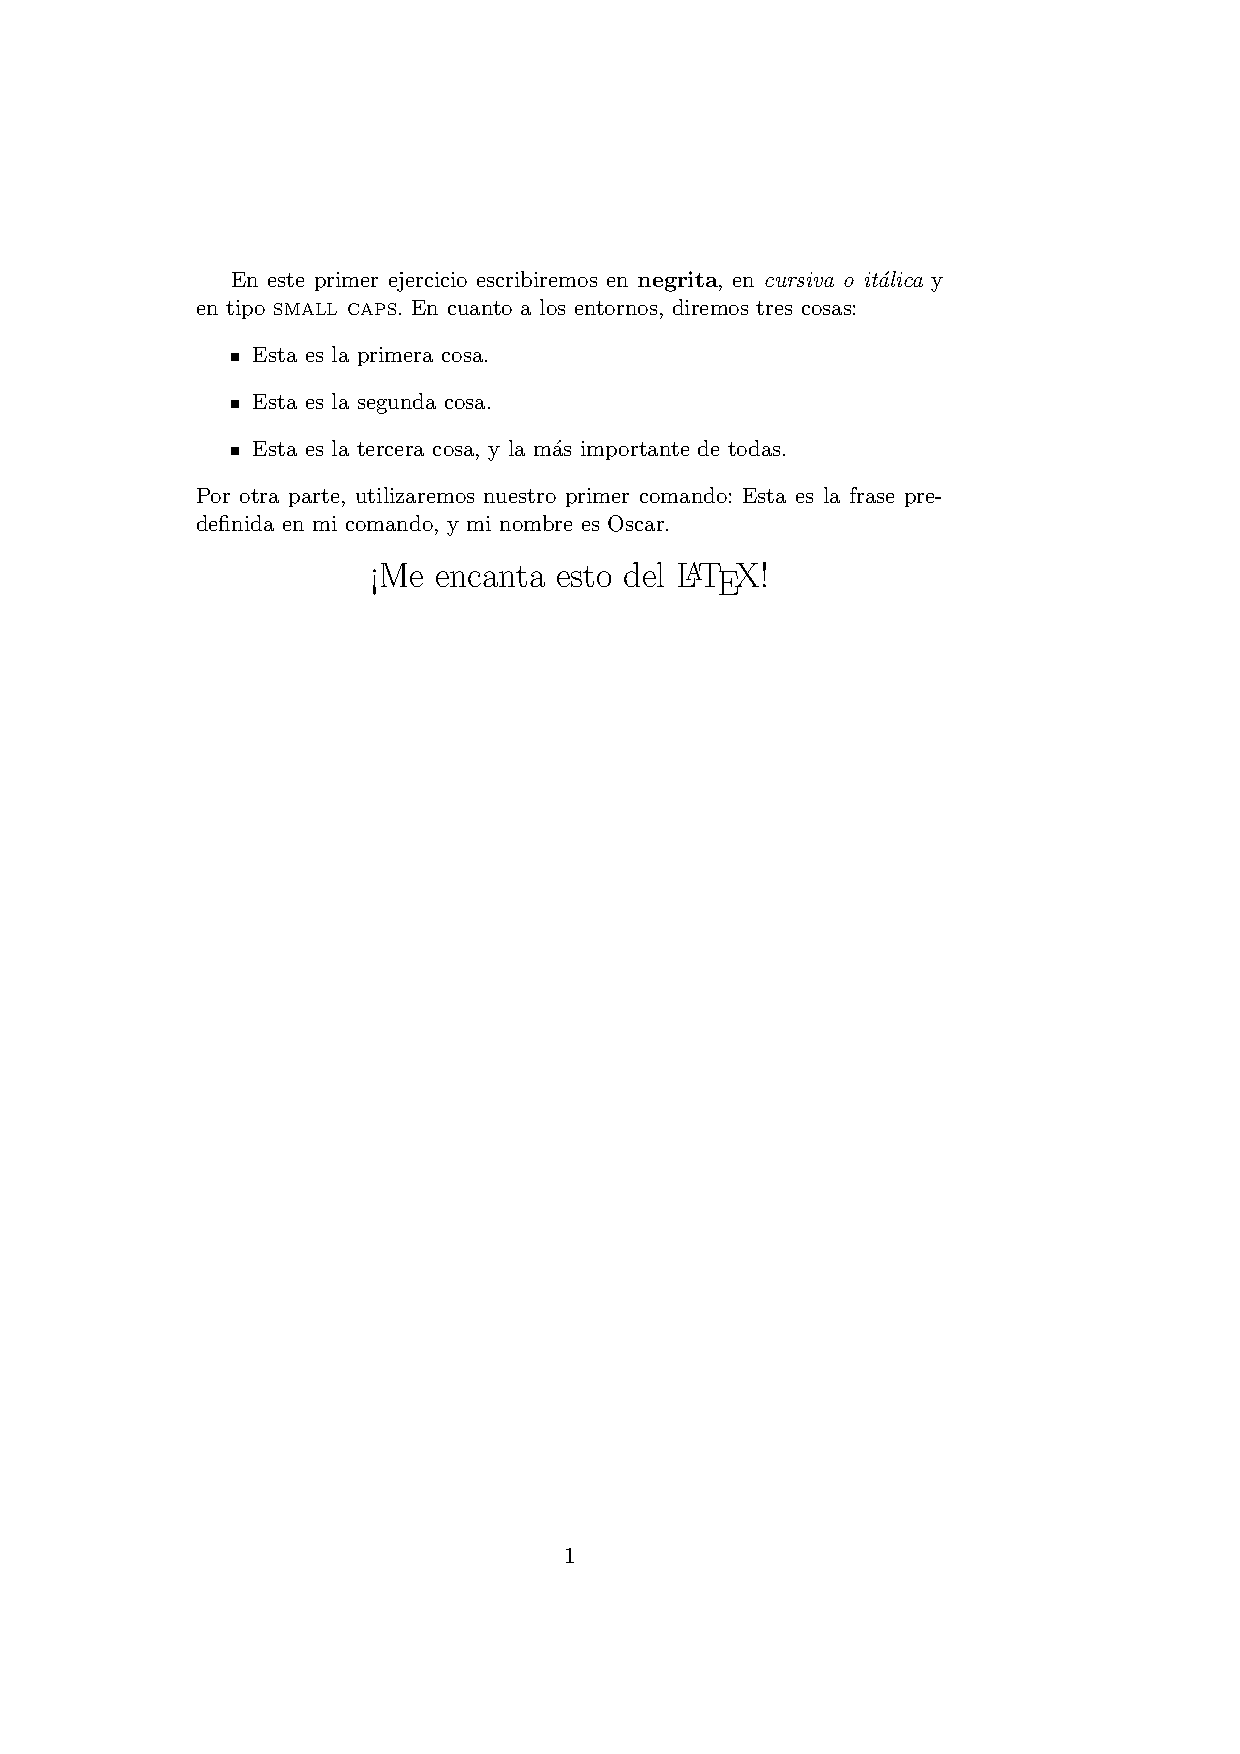
\includegraphics[height=0.9\textheight, page=1]{FigurasEjemplos/Ejercicio1}}
\end{figure}
\end{center}
}
\end{frame}

\begin{frame}[fragile]{Nuestro ejemplo: Report}
\vspace{-0.5cm}
\begin{lstlisting}
%PAQUETES Y CONFIGURACI�N DEL DOCUMENTO (PRE�MBULO)
\documentclass[11pt, twoside, a4paper]{report}
\usepackage[latin1]{inputenc}
\usepackage[spanish]{babel}
\newcommand{\micomando}[1]{Esta es la frase predefinida en mi comando, y mi nombre es #1}
%EL CUERPO
\begin{document}
%Contenido
En este primer ejercicio escribiremos en {\bf negrita}, en {\it cursiva o it�lica} y en tipo {\sc small caps}. En cuanto a los entornos, diremos tres cosas:
\begin{itemize}
\item Esta es la primera cosa.
\item Esta es la segunda cosa.
\item Esta es la tercera cosa, y la m�s importante de todas.
\end{itemize}
Por otra parte, utilizaremos nuestro primer comando: \micomando{Oscar}.
\begin{center}
{\LARGE �Me encanta esto del \LaTeX{}!}
\end{center}
\end{document}
\end{lstlisting}%

\end{frame}


\section{Partes del documento}
\begin{frame}{Las partes del documento}
\only<1>{\centering Todo tiene su lugar: los art�culos, memorias y libros tienen estructuras distintas, por lo que hay que discernir entre los elementos que componen cada una de ellos.}

\only<2->{
De forma general, para los art�culos, {\em reports} y libros, los contenidos ser�n (\alert{orientativo}):
\begin{center}
\uncover<3->{\begin{minipage}{0.25\textwidth}
\begin{acla}{Art�culo}
\begin{center}
{\only<6->{\color{red}}T�tulo\\
Autor\\
Resumen ({\em abstract})\\}
{\only<7->{\color{green}}Cuerpo\\}
{\only<8->{\color{blue}}Agradecimientos\\
Referencias}
\end{center}
\end{acla}
\end{minipage}%
\hfill}
\uncover<4->{\begin{minipage}{0.25\textwidth}
\begin{acla}{Memoria}
\begin{center}
{\only<6->{\color{red}}Portada\\
Dedicatoria\\
Resumen ({\em abstract})\\
Agradecimientos\\
�ndices\\
Pr�logo\\}
{\only<7->{\color{green}}Cap�tulos\\}
{\only<8->{\color{blue}}Ap�ndices\\
Bibliograf�a\\
Glosario}
\end{center}
\end{acla}
\end{minipage}%
\hfill}
\uncover<5->{\begin{minipage}{0.25\textwidth}
\begin{acla}{Libro}
\begin{center}
{\only<6->{\color{red}}Anteportada\\
Portada\\
Derechos\\
Dedicatoria\\
Agradecimientos\\
Pr�logo\\}
{\only<7->{\color{green}}Cap�tulos\\}
{\only<8->{\color{blue}}Ap�ndices\\
Anexos\\
�ndices alfab�ticos}
\end{center}
\end{acla}
\end{minipage}}
\end{center}
}
\only<6->{Pero todos tienen en com�n: }\only<6->{\color{red}\textbf<6>{frontmatter}}\only<7->{{\color{black},}\color{green}\textbf<7>{mainmatter}} \only<8->{{\color{black}y} {\color{blue}\textbf<8>{backmatter}}}
\end{frame}


\subsection{Portada}

\begin{frame}[fragile]{La portada (I)}
\only<1->{Para generar un t�tulo existe \texttt{\backS maketitle} que se sirve de los campos que le preceden}

\only<2->{
\begin{itemize}
\item \alert<2>{\textbf<2>{\texttt{\backS title\{}{\em El t�tulo}\texttt{\}}}}
\item \alert<3>{\textbf<3>{\texttt{\backS author\{}{\em El autor}\texttt{\}}}}
\item \alert<4>{\textbf<4>{\texttt{\backS date\{}{\em La fecha (recomiendo el comando \texttt{\backS today})}\texttt{\}}}}
\item \alert<5>{\textbf<5>{\texttt{\backS thanks\{}{\em Nota al pie de p�gina}\texttt{\}}}}
\end{itemize}
}
\visible<6->{
\begin{minipage}{0.35\textwidth}
\begin{sintax}{\texttt{\backS maketitle}}
 \texttt{[{\em campos previos}]}\\

...

\texttt{\backS maketitle}
\end{sintax}
\end{minipage}}%
\pause\pause\pause\pause\pause\pause%
\hfill%
\begin{minipage}{0.6\textwidth}
\begin{ejem}{\texttt{\backS maketittle}}
\vspace{-0.5cm}
\begin{lstlisting}
\documentclass[a4paper, 10pt]{report}
\title{Sobre la distribuci�n de perros en Gand�a}
\author{Jaimito Garc�a\thanks{El amo de los perros}}
\date{\today}
\begin{document}
\maketitle
% . . . 
\end{document}
\end{lstlisting}
\end{ejem}
\end{minipage}


\end{frame}


\begin{frame}[fragile]{La portada (II)}
Tambi�n est� el entorno \texttt{titlepage}, que permite hacer m�s de una portada:
\pause

\begin{minipage}{0.3\textwidth}
\begin{sintax}{\texttt{titlepage}}
 \texttt{\backS begin\{titlepage\}}\\
{\em Texto con formato} \\
\texttt{\backS end\{titlepage\}}
\end{sintax}
\end{minipage}%
\pause
\hfill
\begin{minipage}{0.6\textwidth}
\begin{ejem}{\texttt{\backS titlepage}}
\vspace{-0.5cm}
\begin{lstlisting}
\documentclass[a4paper, 10pt]{report}
% . . .
\begin{document}
\begin{titlepage}
\begin{center}
\vfill
{\LARGE UNIVERSIDAD POLIT�CNICA DE MADRID}
\vspace{1cm}
{\sc{\Huge Grado en Ingenier�a Electr�nica y Autom�tica}}
\vspace{1cm}
{\Large Jaimito Garc�a}
\vfill
\end{center}
\end{titlepage}
% . . .
\end{document}
\end{lstlisting}
\end{ejem}
\end{minipage}
\end{frame}


\subsection{�ndices}

\begin{frame}[fragile]{Los �ndices}
B�sicamente hay tres tipos de �ndices:
\only<2->{
\begin{itemize}
\item �ndice de contenidos, {\sc toc}  ({\em table of contents})
\item �ndice de figuras
\item �ndice de cuadros
\end{itemize}}

\only<3->{Para incluirlos se escribe simplemente el comando correspondiente a cada uno. \alert<4->{\textbf<4->{\LaTeX{} se encarga de hacer el resto}}.}

\begin{minipage}{0.35\textwidth}
\only<5->{
\begin{sintax}{�ndice de contenidos}
 \texttt{\backS tableofcontents}
\end{sintax}
}
\only<6->{
\begin{sintax}{�ndice de figuras}
 \texttt{\backS listoffigures}
\end{sintax}
}
\only<7->{
\begin{sintax}{�ndice de tablas}
 \texttt{\backS listoftables}
\end{sintax}
}
\end{minipage}%
\pause\pause\pause\pause\pause\pause\pause%
\hfill%
\begin{minipage}{0.6\textwidth}
\begin{ejem}{Los �ndices}
\vspace{-0.5cm}
\begin{lstlisting}
\documentclass[a4paper, 10pt]{report}
% . . . 
\begin{document}
% . . . 
%CONTENIDO
\tableofcontents
%FIGURAS
\listoffigures
%TABLAS
\renewcommand\listtablename{�ndice de tablas} % no de cuadros
\listoftables
% . . . 
\end{document}
\end{lstlisting}
\end{ejem}
\end{minipage}
\end{frame}

\subsection{Resumen}

\begin{frame}[fragile]{El resumen o {\em abstract}}
Esta parte solo se puede a�adir en \alert<1>{documentos de tipo art�culo o memoria}. En los \alert<1>{libros}, el entorno que se emplea \alert<1>{no est� disponible}.

\pause
\begin{minipage}{0.3\textwidth}
\begin{sintax}{\texttt{\backS abstract}}
 \texttt{\backS begin\{abstract\}}\\
{\em Texto del resumen} \\
\texttt{\backS end\{abstract\}}
\end{sintax}
\end{minipage}%
\pause%
\hfill%
\begin{minipage}{0.6\textwidth}
\begin{ejem}{\texttt{\backS abstract}}
\vspace{-0.5cm}
\begin{lstlisting}
\begin{abstract}
Lorem ipsum dolor sit amet, consectetur adipiscing elit. Morbi sagittis tincidunt augue ac vestibulum. Maecenas elementum lorem scelerisque leo adipiscing, non interdum mauris vestibulum. Donec eu quam nec erat dapibus scelerisque lobortis et mauris. Aenean ut molestie mauris.
\end{abstract}
\end{lstlisting}
\end{ejem}
\end{minipage}
\end{frame}

\subsection{Cuerpo}

\begin{frame}{Las partes del cuerpo (I)}
\only<1>{
Existen en  \LaTeX{}  \textbf{\color{miverdeO}instrucciones} para ordenar jer�rquicamente los conceptos e ideas de un documento con el fin de \textbf{\color{miverdeO}organizar} todo.}

\only<2->{Dependiendo del \alert<2>{tipo de documento} se consideran \alert<2>{algunas divisiones} o no}

\only<3->{
\begin{sintax}{Unidades de estructura}
\texttt{\backS {\em instrucci�n}[{\em t�tulo {\sc toc}}]\{{\em t�tulo}\}}

\only<3-8>{
{\centering o bien}

\texttt{\backS {\em instrucci�n}*\{{\em t�tulo}\}}}
\end{sintax}
}
\only<4-8>{
La sintaxis con asterisco (\alert<4>{\textbf<4>{*}}) sirve para \alert<4>{\textbf<4>{evitar}} que la unidad se \alert<4>{\textbf<4>{numere}} y que \alert<4>{\textbf<4>{aparezca en la {\sc toc}}}.}
\only<5-8>{
\begin{itemize}
\item \alert<6>{\texttt{\em \backS instrucci�n} se refiere a la unidad de estructura}
\item  \alert<7>{\texttt{\em t�tulo {\sc toc}} es el nombre que se mostrar� en la {\sc toc} para esa unidad}
\item \alert<8>{ \texttt{\em t�tulo} es el t�tulo de la unidad}
\end{itemize}
}
\only<9->{
\begin{defi}{Las unidades de estructura}
\begin{table}
{\small
% Table generated by Excel2LaTeX from sheet 'Hoja1'
\begin{tabular}{|l|l|c|c|}
\hline
    Nombre &   Sintaxis &    {\em article} & {\em book} y {\em report} \\
\hline
     Parte &         \texttt{\backS part[t�tulo{\sc toc}]\{t�tulo\}}      &  \neutro (opc.)    &      \neutro (opc.)      \\
\hline
  Cap�tulo &         \texttt{\backS chapter[t�tulo{\sc toc}]\{t�tulo\}}        &    \mal    &   \bien   \\
\hline
   Secci�n &          \texttt{\backS section[t�tulo{\sc toc}]\{t�tulo\}}       &    \bien        &      \bien      \\
\hline
Subsecci�n &         \texttt{\backS subsection[t�tulo{\sc toc}]\{t�tulo\}}         &      \bien      &      \bien      \\
\hline
Subsubsecci�n &        \texttt{\backS subsubsection[t�tulo{\sc toc}]\{t�tulo\}}           &    \bien        &       \bien     \\
\hline
   P�rrafo &           \texttt{\backS paragraph[t�tulo{\sc toc}]\{t�tulo\}}         &      \bien      &      \bien      \\
\hline
Subp�rrafo &         \texttt{\backS subparagraph[t�tulo{\sc toc}]\{t�tulo\}}         &      \bien      &       \bien     \\
\hline
\end{tabular}  
}
\end{table}
\end{defi}
}

\end{frame}

\begin{frame}{Las partes del cuerpo (II)}
Estas instrucciones van en el \alert{cuerpo del documento}, y su alcance va desde su llamada hasta la llamada a otra instrucci�n de estructura.
\end{frame}

\begin{frame}[fragile]{Las partes del cuerpo (II)}
\vspace{-0.2cm}
\begin{ejem}{Unidades de estructura ({\em report}) (I)}
\vspace{-0.5cm}
\begin{lstlisting}
\documentclass[11pt, twoside, a4paper]{report}
\usepackage[latin1]{inputenc}
\usepackage[spanish]{babel}
\begin{document}
\part{La taxonomia de un gato dom�stico}
\chapter{Las tres primeras divisiones}
La taxonom�a es, en su sentido m�s general, la ciencia de la clasificaci�n. Habitualmente, se emplea el t�rmino para %. . .
Las tres primeras divisiones para clasificar, por ejemplo, un gato son: 
\begin{itemize}
\item Dominio: Eucarya
\item Reino: Animalia
\item Subreino: Eumetazoa
\end{itemize}
Referidas a: organismos celulares con n�cleos verdaderos, capacidad de locomoci�n, consumen ox�geno, nutrici�n por ingesti�n, reproducci�n sexual y desarrollo embrionario, presentan tejidos, �rganos, masa corporal, etc.
\section{De forma m�s anidada}
Las siguientes tres divisiones son: 
\begin{itemize}
\item Filo: Chordata
\item Subfilo: Vertebrata  
\item Clase: Mammalia
\end{itemize}
Debido a : existencia de cuerda dorsal, columna vertebral, ser mam�feros que se caracterizan por tener gl�ndulas mamarias, pelo y mand�bulas.
\subsection{A�n m�s anidado}
Las siguientes tres divisiones son: 
\end{lstlisting}
\end{ejem}
\end{frame}


\begin{frame}[fragile]{Las partes del cuerpo (II)}
\vspace{-0.2cm}
\begin{ejem}{Unidades de estructura  ({\em report}) (II)}
\vspace{-0.5cm}
\begin{lstlisting}
\begin{itemize}
\item Subclase: Theria
\item Infraclase: Placentalia
\item Orden: Carn�vora
\end{itemize}
Porque el embri�n se forma en el �tero materno, las cr�as permanecen en el �tero materno durante largo tiempo y los molares est�n adaptados para el consumo de carne.
\subsubsection{Anidad�simo}
Las siguientes tres divisiones son: 
\begin{itemize}
\item Suborden: Feliformia
\item Familia: Felidae
\item Subfamilia: Felinae
\end{itemize}
Debido a su  anatom�a felina, estar entre los grandes y peque�os f�lidos y ser incapaces de rugir.
\paragraph{Al final de la clasificaci�n}
Las siguientes tres divisiones son: 
\begin{itemize}
\item G�nero: Felis
\item Especie: Felis silvestris
\item Subespecie: Felis silvestris catus
\end{itemize}
Porque son Linnaeus, gatos peque�os y finalmente, esa es la denominaci�n de la Comisi�n Internacional de  Nomenclatura Zool�gica
\subparagraph{Finalmente}
La clasificaci�n de los gatos es un ejemplo de la organizaci�n jer�rquica de las ideas, �y ya pod�is ver lo �til que es!
\end{document}
\end{lstlisting}
\end{ejem}

\end{frame}



\begin{frame}[fragile]{Las partes del cuerpo (II)}
\vspace{-0.1cm}
\begin{center}
\only<1->{
\begin{minipage}{0.32\textwidth}
\begin{figure}[hbtp]
\centering
\fbox{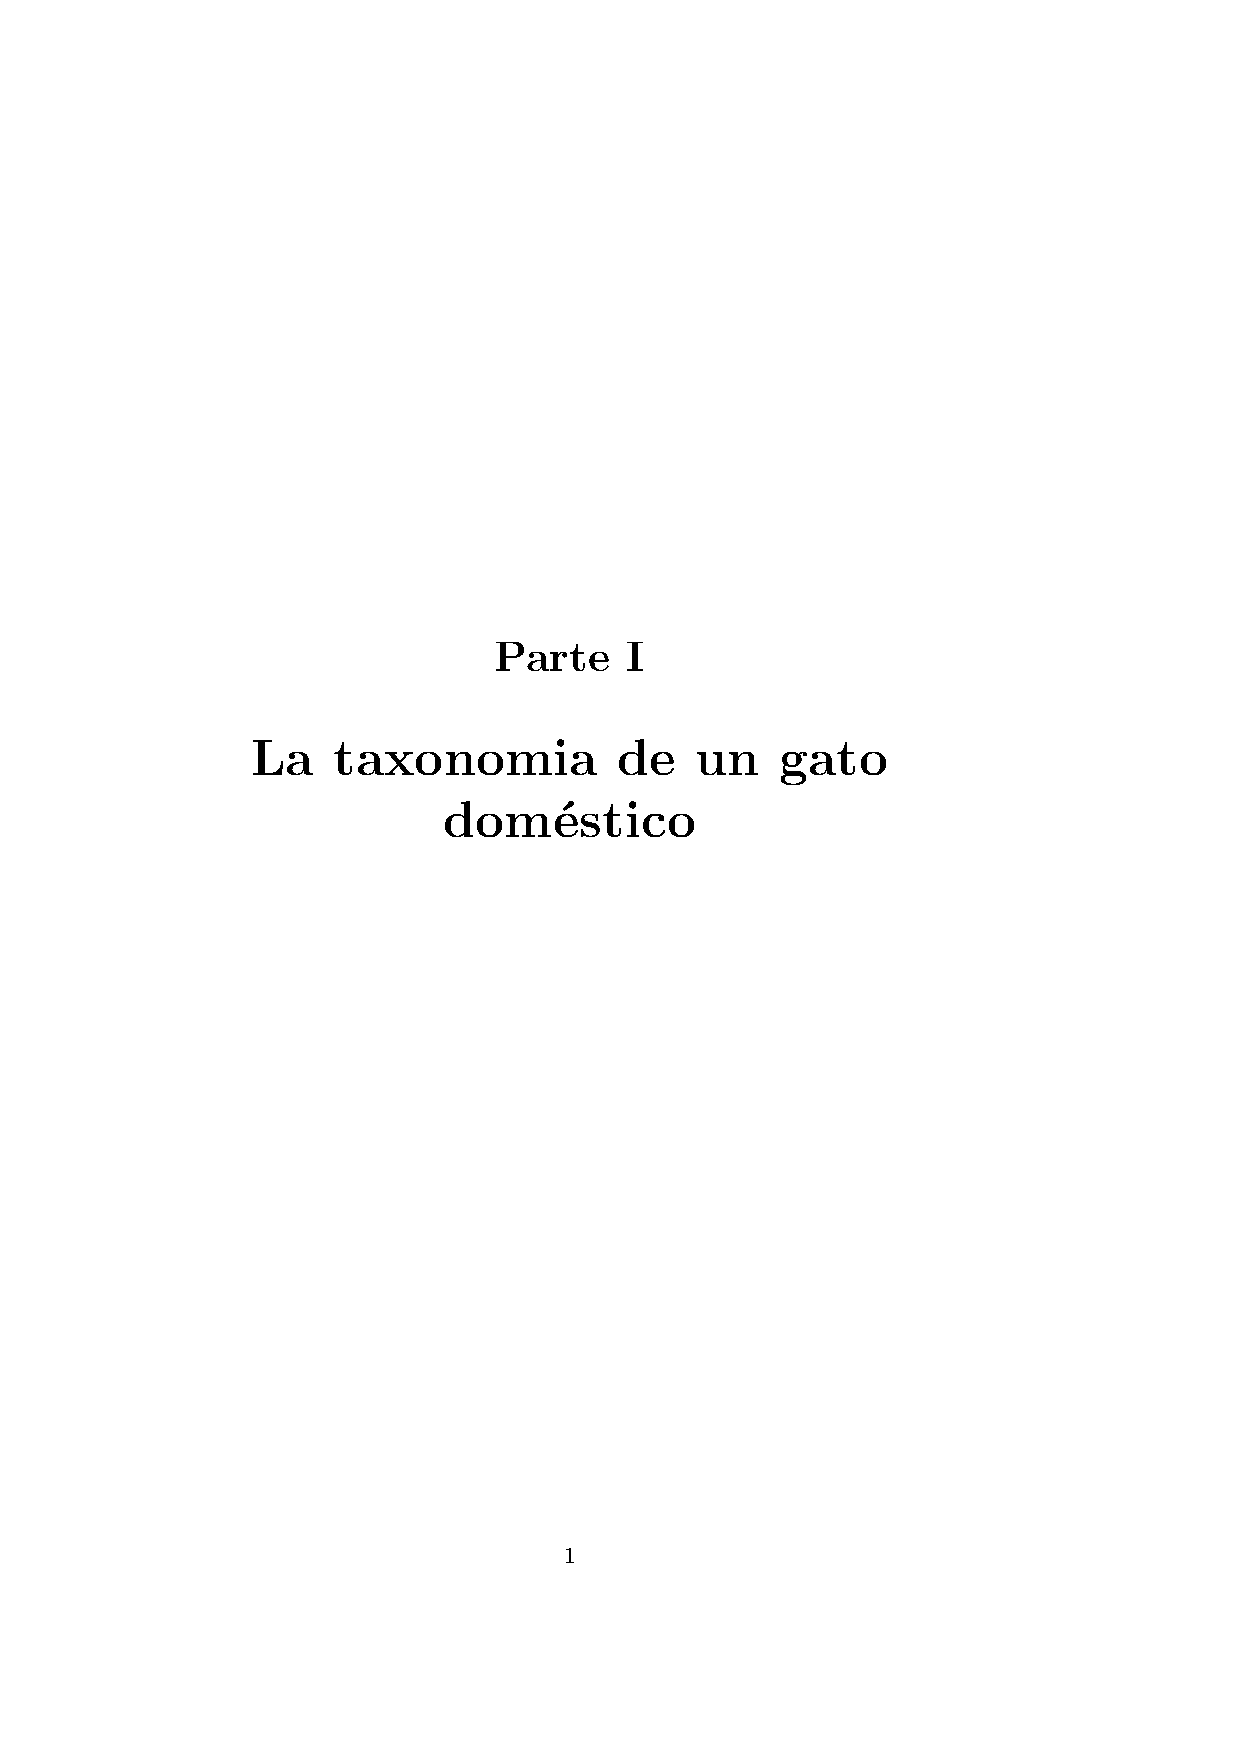
\includegraphics[width=\textwidth, page=1]{FigurasEjemplos/Cuerpo}}
\end{figure}
\end{minipage}}%
\hfill
\only<2->{
\begin{minipage}{0.32\textwidth}
\begin{figure}[hbtp]
\centering
\fbox{\includegraphics[width=\textwidth, page=2]{FigurasEjemplos/Cuerpo}}
\end{figure}
\end{minipage}}%
\hfill
\only<3->{
\begin{minipage}{0.32\textwidth}
\begin{figure}[hbtp]
\centering
\fbox{\includegraphics[width=\textwidth, page=3]{FigurasEjemplos/Cuerpo}}
\end{figure}
\end{minipage}}%
\end{center}
\end{frame}

\subsection{Anexos}

\begin{frame}[fragile]{Los anexos}

La forma de escribir un anexo es muy parecida a la del resto de elementos del cuerpo. \visible<2->{{\color{miverdeO}De hecho es igual}, pero hay que indicar que lo que viene a continuaci�n se debe tratar como anexos.}

\visible<3->{La manera de avisar a \LaTeX{} es mediante el comando \texttt{\backS appendix}}

\visible<4->{
\begin{minipage}{0.42\textwidth}
\begin{sintax}{\texttt{\backS appendix}}
\texttt{\backS appendix}\\
\texttt{\backS chapter\{}{\em T�tulo del primer ap�ndice}\texttt{\}}\\
\vdots
\end{sintax}
\end{minipage}}%
\pause\pause\pause\pause%
\hfill%
\begin{minipage}{0.49\textwidth}
\begin{ejem}{\texttt{\backS appendix}}
\vspace{-0.5cm}
\begin{lstlisting}
\documentclass[a4paper, 10pt]{report}
\usepackage[latin1]{inputenc}
\usepackage[spanish]{babel}
\begin{document}
% . . . 
\appendix
\chapter{Acerca de los m�todos empleados}
\section{Sobre los datos a los que se hace referencia en el cap�tulo 2}
% . . . 
\end{document}
\end{lstlisting}
\end{ejem}
\end{minipage}


\end{frame}



\subsection{Bibliograf�a}

\begin{frame}{La bibliograf�a (I)}
\begin{itemize}
\item <1-> Aparece {\color{miverdeO}al final} del documento de forma {\color{miverdeO}ordenada y/o numerada} seg�n un criterio
\item <2-> Las referencias se hacen mediante etiquetas, que \LaTeX{} enlaza autom�ticamente
\item <3-> El entorno para la bibliograf�a se llama \alert<3>{\texttt{thebibliography}}
\item <4-> La manera de referenciar es mediante el comando \alert<4>{\texttt{\backS cite}}
\end{itemize}

\visible<5->{
\begin{minipage}{0.58\textwidth}
\begin{sintax}{\texttt{thebibliography}}
\texttt{\backS begin\{thebibliography\}\{{\em long. m�xima}\}}\\
\vdots

\texttt{\backS bibitem[{\em leyenda}]\{{\em etiqueta}\} \{{\em texto}\}}

\vdots

\texttt{\backS end\{thebibliography\}}\\
\end{sintax}
\end{minipage}}%
\visible<6->{
\hfill
\begin{minipage}{0.39\textwidth}
\begin{sintax}{\texttt{cite}}
\texttt{\backS cite[{\em opcional}]\{{\em etiqueta}\}}\\
\end{sintax}
\only<7->{\texttt{{\em opcional}} es un texto que se puede a�adir a la referencia cuando es llamada.}
\end{minipage}%
}
\only<8>{
\vfill
Existe otro m�todo  mediante el comando  \alert<8>{\texttt{\backS bibliography}} que se complementa con el formato de archivos \alert<8>{\textbf<8>{BIB\TeX{}}}}
\end{frame}

\begin{frame}[fragile]{La bibliograf�a (II)}
\begin{ejem}{\texttt{thebibliography}}
\vspace{-0.5cm}
\begin{lstlisting}
\begin{thebibliography}{99}
\addcontentsline{toc}{chapter}{Bibliograf�a}
\bibitem{Mathews, Fink}{\bf Mathews, J. H., Fink, K. T.} {\it (2008) M�todos num�ricos con MATLAB, 3� edici�n. Prentice-Hall.}
\bibitem{Faires, Burden}{\bf Faires, J.D., Burden, R.} {\it (2004) M�todos num�ricos, 3� edici�n. Thomson.}
\bibitem{Mantilla}{\bf Ignacio Mantilla} {\it An�lisis num�rico.} Universidad Nacional de Colombia
\bibitem{Kreyszig}{\bf E.Kreyszig} {\it Matem�ticas Avanzadas para Ingenieros. Limusa, M�xico.}
\bibitem{Zapateiro, Fernandez} {\bf Zapateiro, J. V., Fern�ndez, V. O.}{\it An�lisis num�rico. Notas de clase. Uninorte.}
\end{thebibliography}
\end{lstlisting}
\end{ejem}
\pause
\vspace{-0.2cm}
\begin{figure}
\centering
\begin{tikzpicture}
\alt<2->{\node[opacity=1]{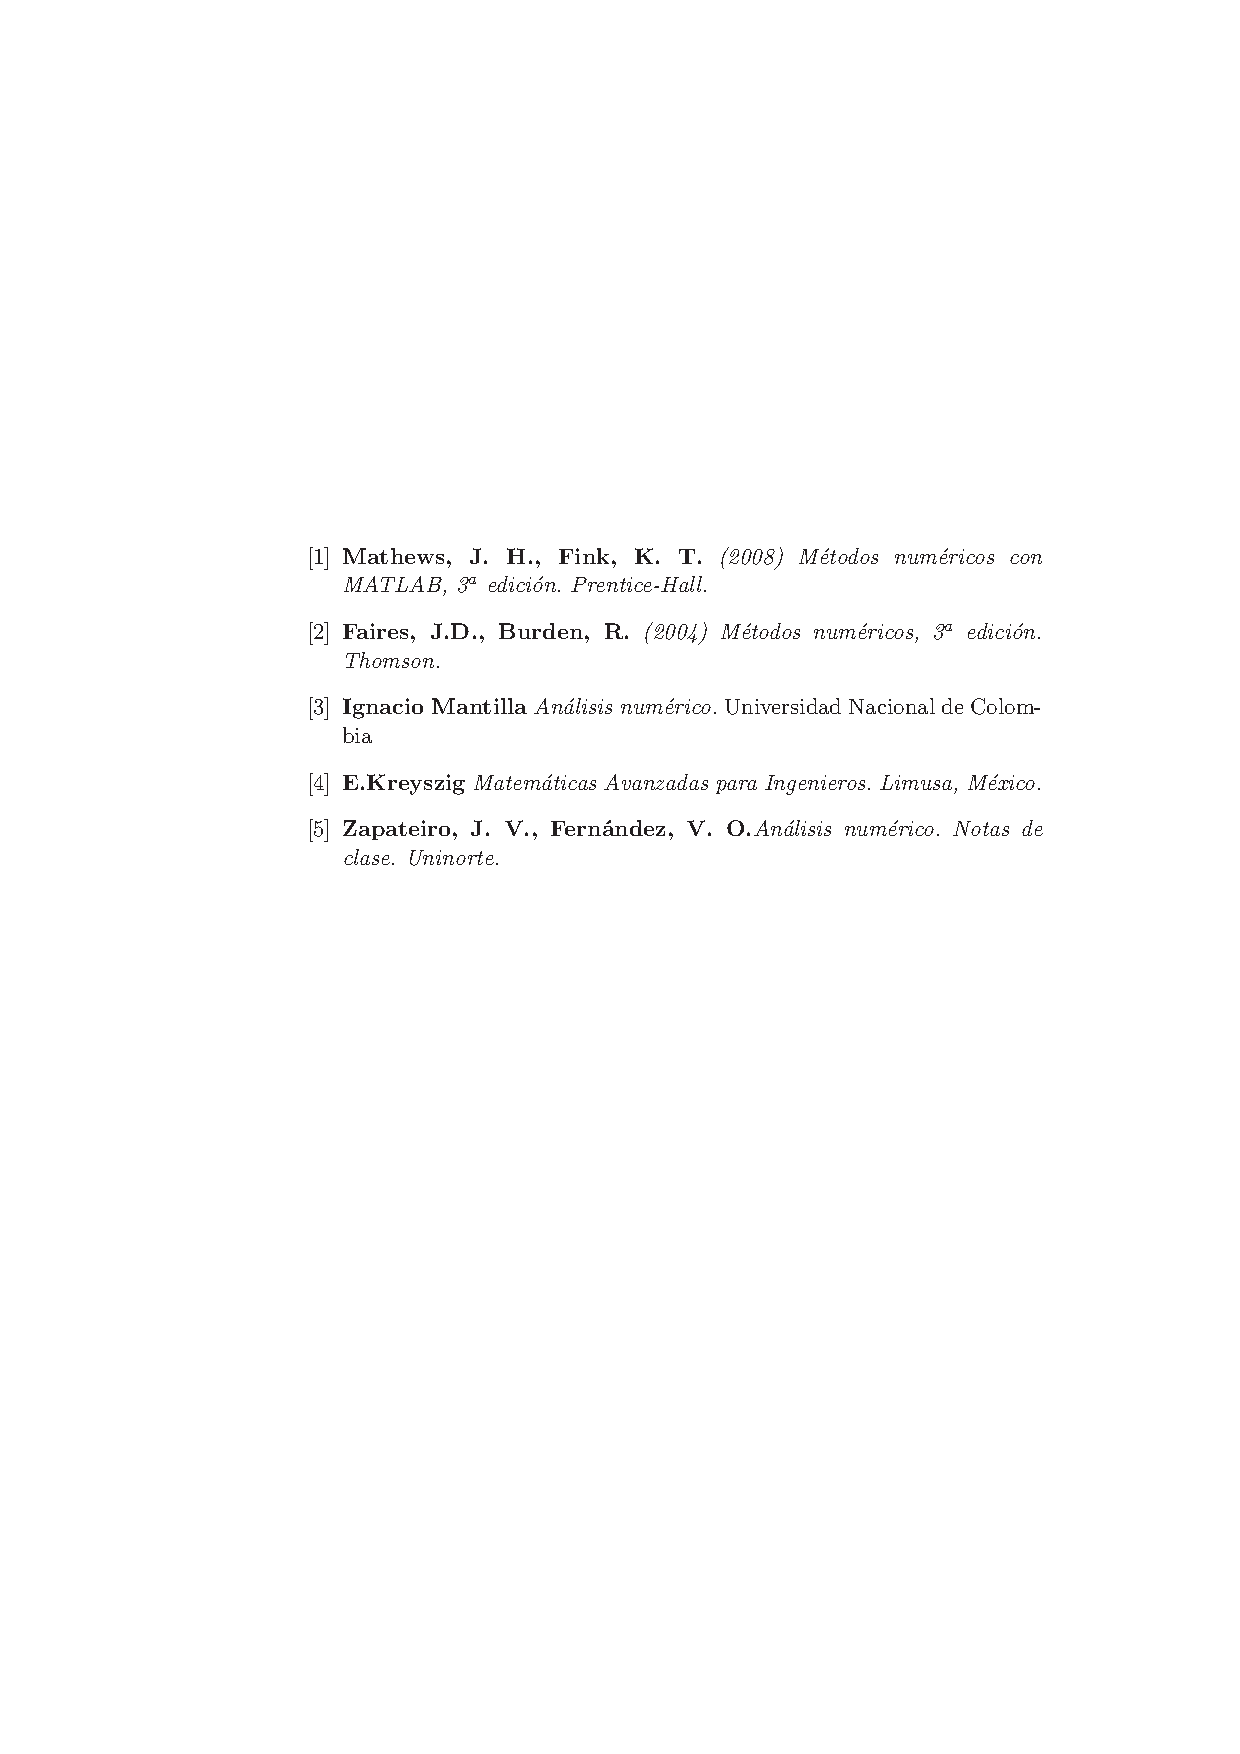
\includegraphics[height=0.4\textheight]{FigurasEjemplos/bibliografia2}};}
{\node[opacity=0.01]{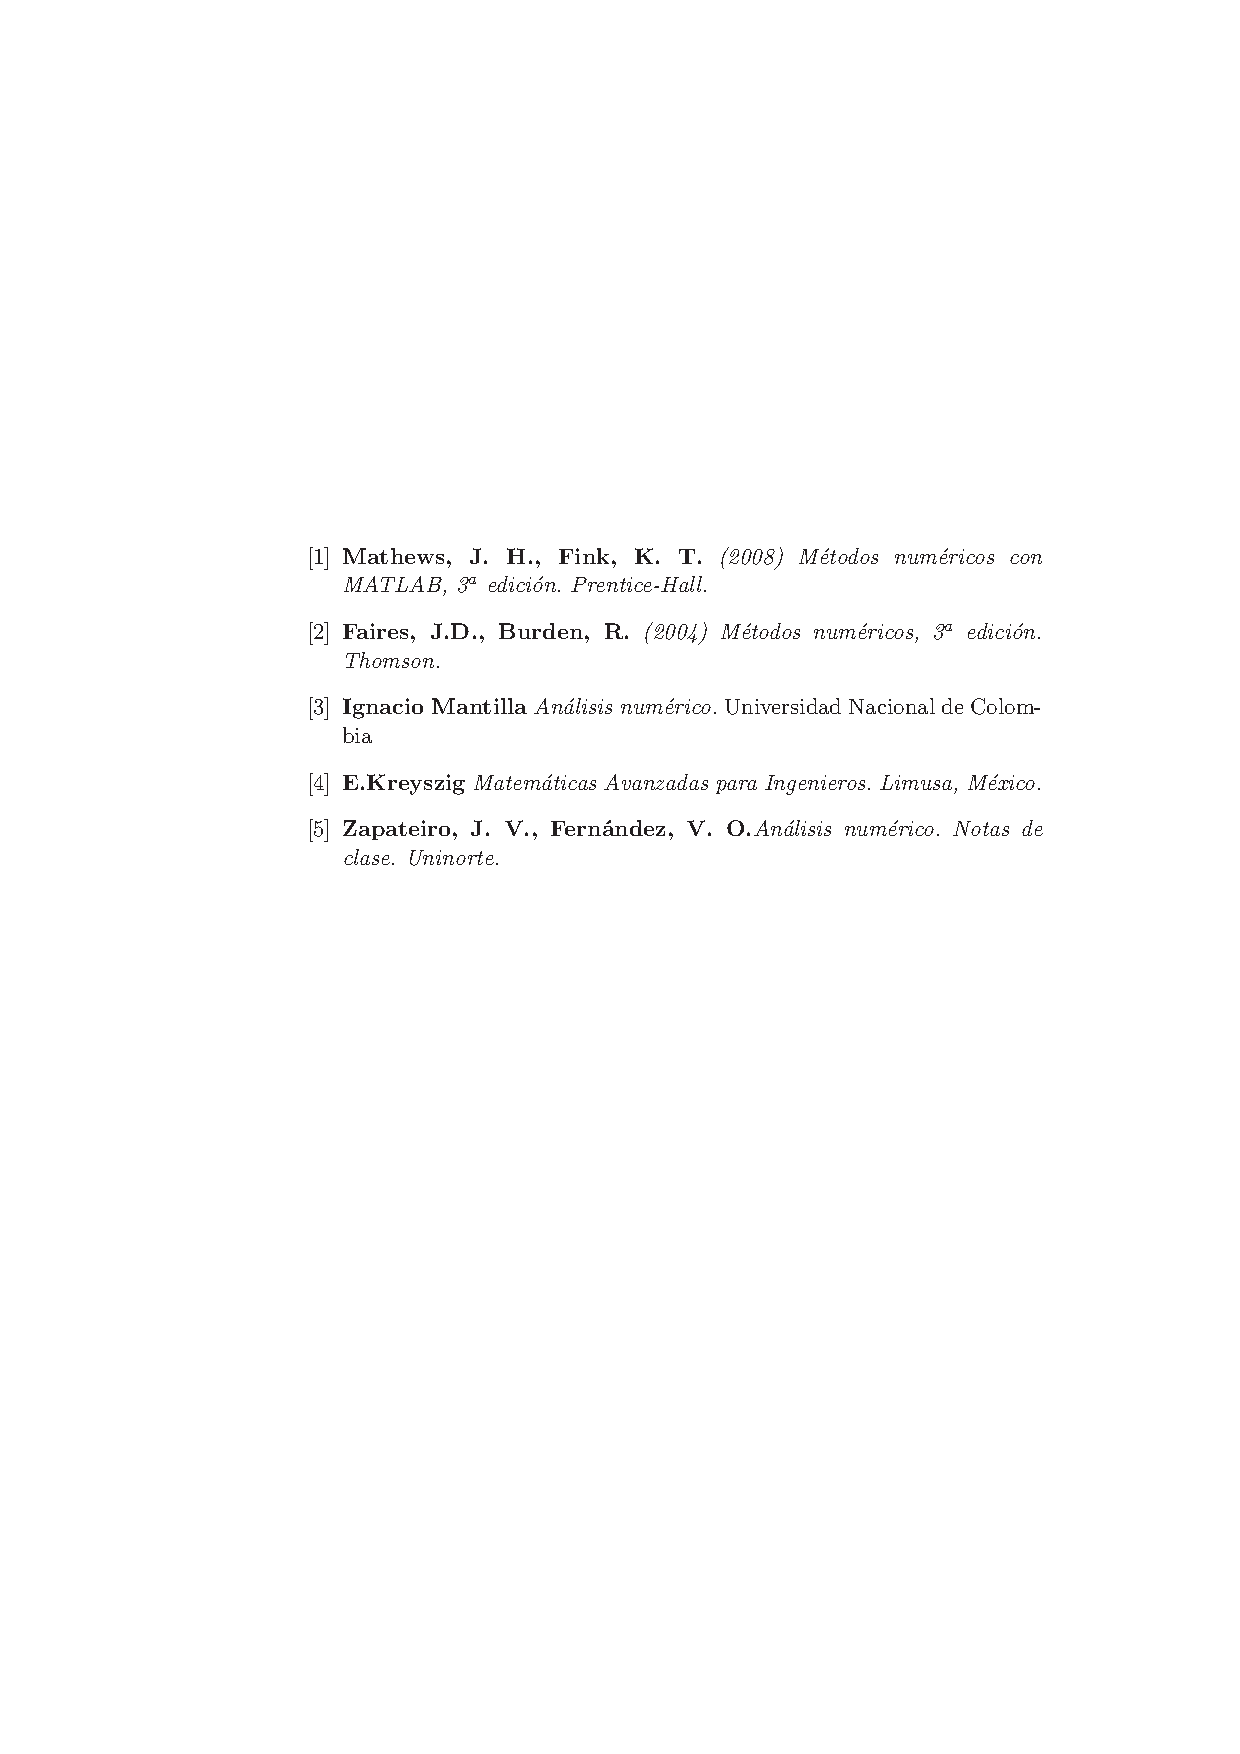
\includegraphics[height=0.4\textheight]{FigurasEjemplos/bibliografia2}};}
\end{tikzpicture}
\end{figure}
\end{frame}



\subsection{�Manos a la obra!}

\begin{frame}[fragile]{Nuestro ejemplo: Report }
\vspace{-0.1cm}
\begin{center}
\only<1->{
\begin{minipage}{0.32\textwidth}
\begin{figure}[hbtp]
\centering
\fbox{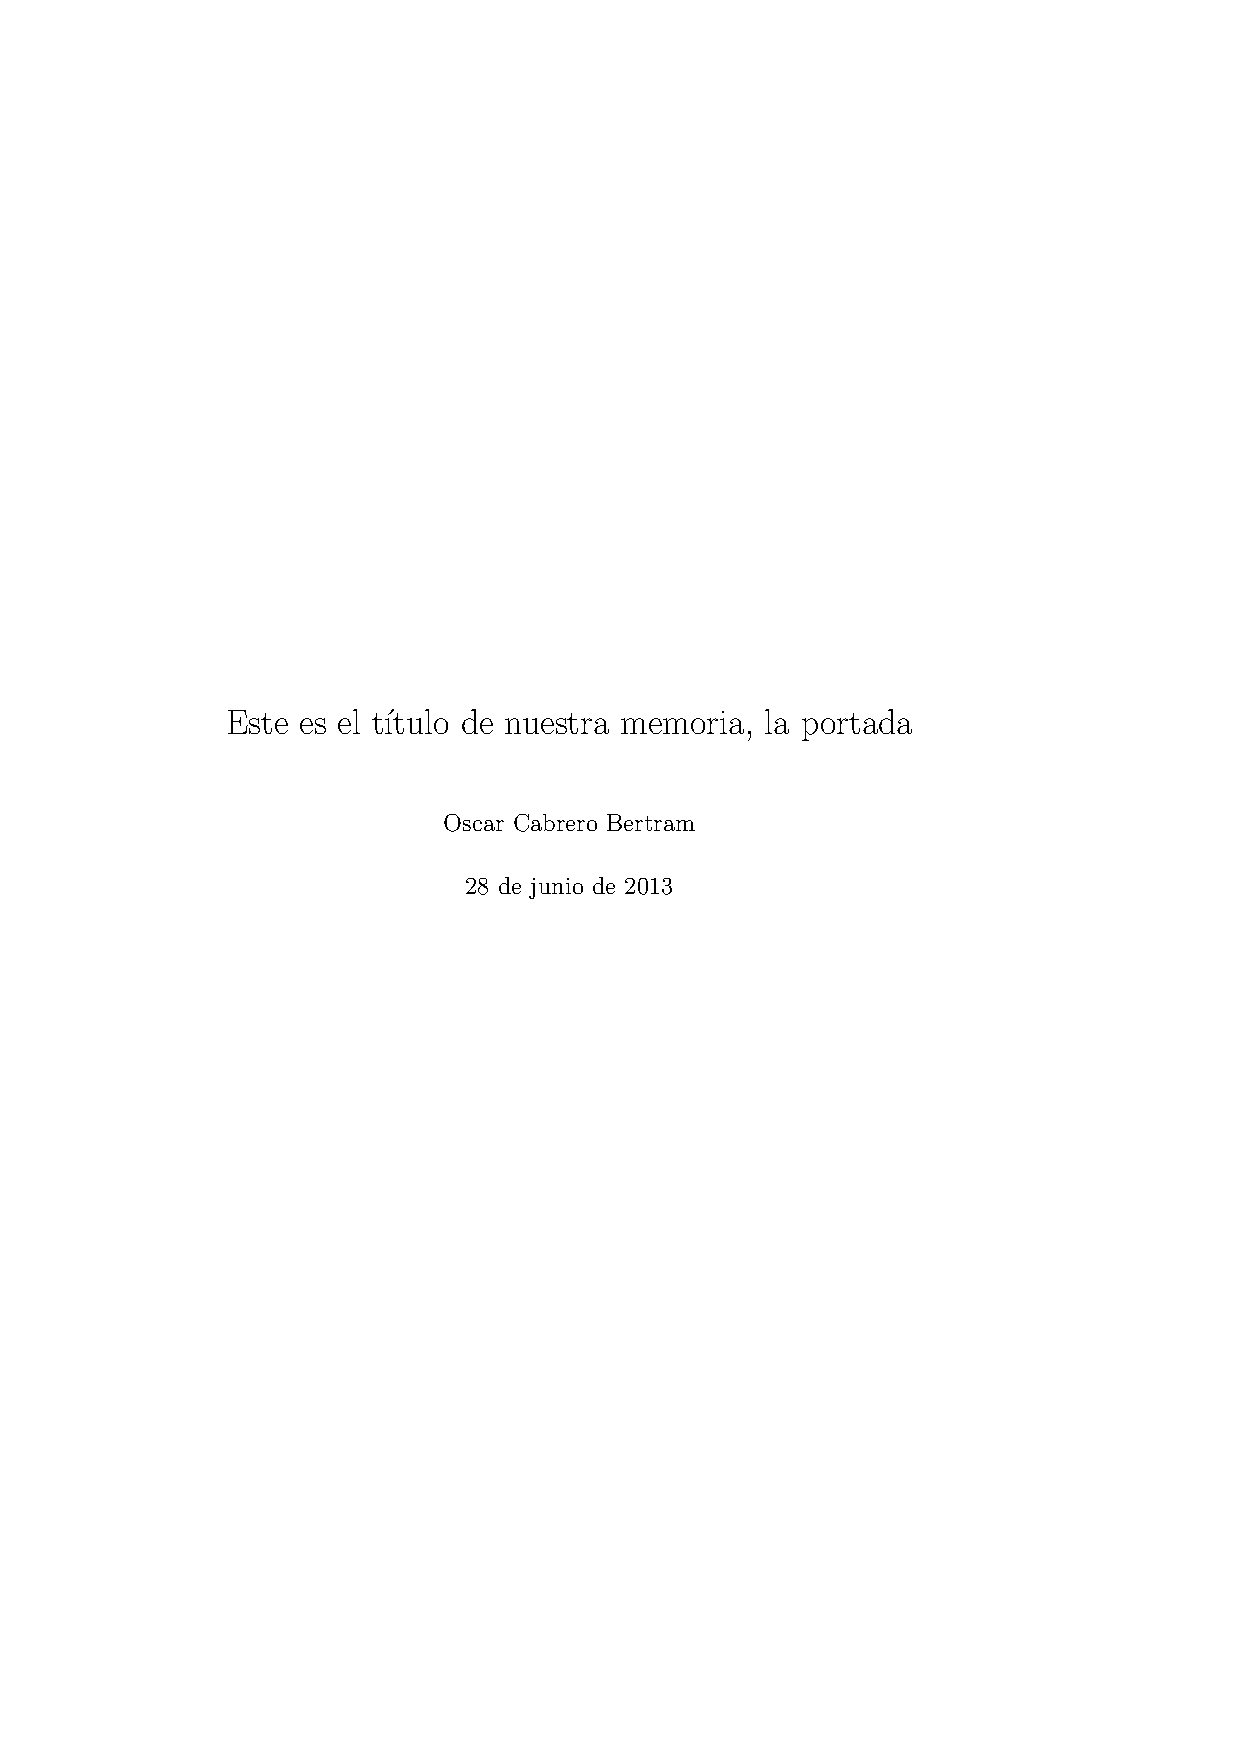
\includegraphics[width=\textwidth, page=1]{FigurasEjemplos/Ejercicio2}}
\end{figure}
\end{minipage}}%
\hfill
\only<2->{
\begin{minipage}{0.32\textwidth}
\begin{figure}[hbtp]
\centering
\fbox{\includegraphics[width=\textwidth, page=2]{FigurasEjemplos/Ejercicio2}}
\end{figure}
\end{minipage}}%
\hfill
\only<3->{
\begin{minipage}{0.32\textwidth}
\begin{figure}[hbtp]
\centering
\fbox{\includegraphics[width=\textwidth, page=3]{FigurasEjemplos/Ejercicio2}}
\end{figure}
\end{minipage}}%
\end{center}
\end{frame}

\begin{frame}[fragile]{Nuestro ejemplo: Report }
\vspace{-0.1cm}
\begin{center}
\only<1->{
\begin{minipage}{0.32\textwidth}
\begin{figure}[hbtp]
\centering
\fbox{\includegraphics[width=\textwidth, page=4]{FigurasEjemplos/Ejercicio2}}
\end{figure}
\end{minipage}}%
\hfill
\only<2->{
\begin{minipage}{0.32\textwidth}
\begin{figure}[hbtp]
\centering
\fbox{\includegraphics[width=\textwidth, page=5]{FigurasEjemplos/Ejercicio2}}
\end{figure}
\end{minipage}}%
\hfill
\only<3->{
\begin{minipage}{0.32\textwidth}
\begin{figure}[hbtp]
\centering
\fbox{\includegraphics[width=\textwidth, page=6]{FigurasEjemplos/Ejercicio2}}
\end{figure}
\end{minipage}}%
\end{center}
\end{frame}



\begin{frame}[fragile]{Nuestro ejemplo: Report}
\vspace{-0.5cm}
\begin{lstlisting}
%PAQUETES Y CONFIGURACI�N DEL DOCUMENTO (PRE�MBULO)
\documentclass[11pt, twoside, a4paper]{report}
\usepackage[latin1]{inputenc}
\usepackage[spanish]{babel}
\newcommand{\micomando}[1]{Esta es la frase predefinida en mi comando, y mi nombre es #1}
%	EL CUERPO
\begin{document}
% Antes de nada...
\title{Este es el t�tulo de nuestra memoria, la portada}
\author{Oscar Cabrero Bertram}
\date{\today}  
\maketitle
%�ndice
\tableofcontents
%Resumen
\begin{abstract}
Este es mi primer res�men. Me parece raro que solo tenga que preocuparme por lo que quiero decir, y no por c�mo tengo que presentarlo. En esta memoria expondremos la mayor parte de las cosas que hemos aprendido en este curso.
\end{abstract}
%Contenido
\chapter{Mi primer cap�tulo}
Este es el p�rrafo de entrada a mi primer cap�tulo. A continuaci�n se presenta la primera secci�n en \LaTeX{}.
\section{Mi primera secci�n}
En este primer ejercicio escribiremos en {\bf negrita}, en {\it cursiva o it�lica} y en tipo {\sc small caps}. En cuanto a los entornos, diremos tres cosas:
\end{lstlisting}%
\end{frame}

\begin{frame}[fragile]{Nuestro ejemplo: Report}
\vspace{-0.5cm}
\begin{lstlisting}
\begin{itemize}
\item Esta es la primera cosa.
\item Esta es la segunda cosa.
\item Esta es la tercera cosa, y la m�s importante de todas.
\end{itemize}
Por otra parte, utilizaremos nuestro primer comando: \micomando{Oscar}.
\begin{center}
{\LARGE �Me encanta esto del \LaTeX{}!}
\end{center
\subsection{Mi primera subsecci�n}
Esta es mi primera subsecci�n, y tiene un p�rrafo:
\paragraph{Primer p�rrafo} En este p�rrafo tengo que decir que estoy muy contento por todo lo que he aprendido en \cite{Cabrero}
%Ap�ndices
\appendix
\chapter{Informaci�n adicional}
Aqu� iremos poniendo informaci�n que complemente al documento general.
%Bibliograf�a
\begin{thebibliography}{99}
\addcontentsline{toc}{chapter}{Bibliograf�a}
\bibitem{Cabrero}{\bf Cabrero Bertram, O} {\it (2013) Diapositivas de clase}
\end{thebibliography}
\end{document}
\end{lstlisting}%

\end{frame}




\section{Entornos}

\subsection{Listas}

\begin{frame}{Los tipos de listas}
\only<1>{\begin{quote}
Creo en las listas, me encantan. Soy ingeniero industrial, de ah� que ame los n�meros y si amas los n�meros, amas las listas.
\end{quote}
\begin{flushright} Albert Espinosa \end{flushright}}
\only<2-5>{
\begin{itemize}
\item <2-> \alert<2>{Las listas sirven para presentar informaci�n estructurada}
\item <3-> \alert<3>{Pueden anidarse}
\item <4-> \alert<4>{\LaTeX{} se encarga de los contadores y de las sangr�as relativas}
\item <5-> Tipos de listas:
\begin{itemize}
\item Listas con vi�etas
\item Listas numeradas
\item Listas descriptivas
\end{itemize}
\end{itemize}
}
\end{frame}

\begin{frame}[fragile]{Listas de tipo vi�etas}
\only<1->{
\begin{minipage}{0.65\textwidth}
\begin{itemize}
\item <1->{Los diferentes \alert<1->{\textbf<1>{�tems}} se identifican mediante una vi�eta o \alert<1->{marca com�n}}

\item <2->{El entorno empleado se denomina \texttt{itemize}}
\end{itemize}
\end{minipage}}%
\hfill%
\only<3->{
\begin{minipage}{0.3\textwidth}
\begin{sintax}{\texttt{itemize}}
 \texttt{\backS begin\{itemize\}}\\
\texttt{\backS item }{\em Texto 1}  \\
\texttt{\backS item }{\em Texto 2}  \\

\vdots

\texttt{\backS end\{itemize\}}
\end{sintax}
\end{minipage}
}
\pause\pause\pause

\begin{minipage}{0.4\textwidth}
\vspace{-1cm}
\begin{ejem}{\texttt{itemize}}
\vspace{-0.5cm}
\begin{lstlisting}
\begin{itemize}
\item Pan
\item Leche
\item Huevos
\item Carnicer�a:
\begin{itemize}
\item Pollo
\item Jam�n serrano
\item Hamburguesas
\end{itemize}
\item Refrescos
\end{itemize}
\end{lstlisting}
\end{ejem}
\end{minipage}%
\pause%
\hspace{1cm}%
\begin{minipage}{0.4\textwidth}
\begin{figure}
\centering
\begin{tikzpicture}
\alt<5->{\node[opacity=1]{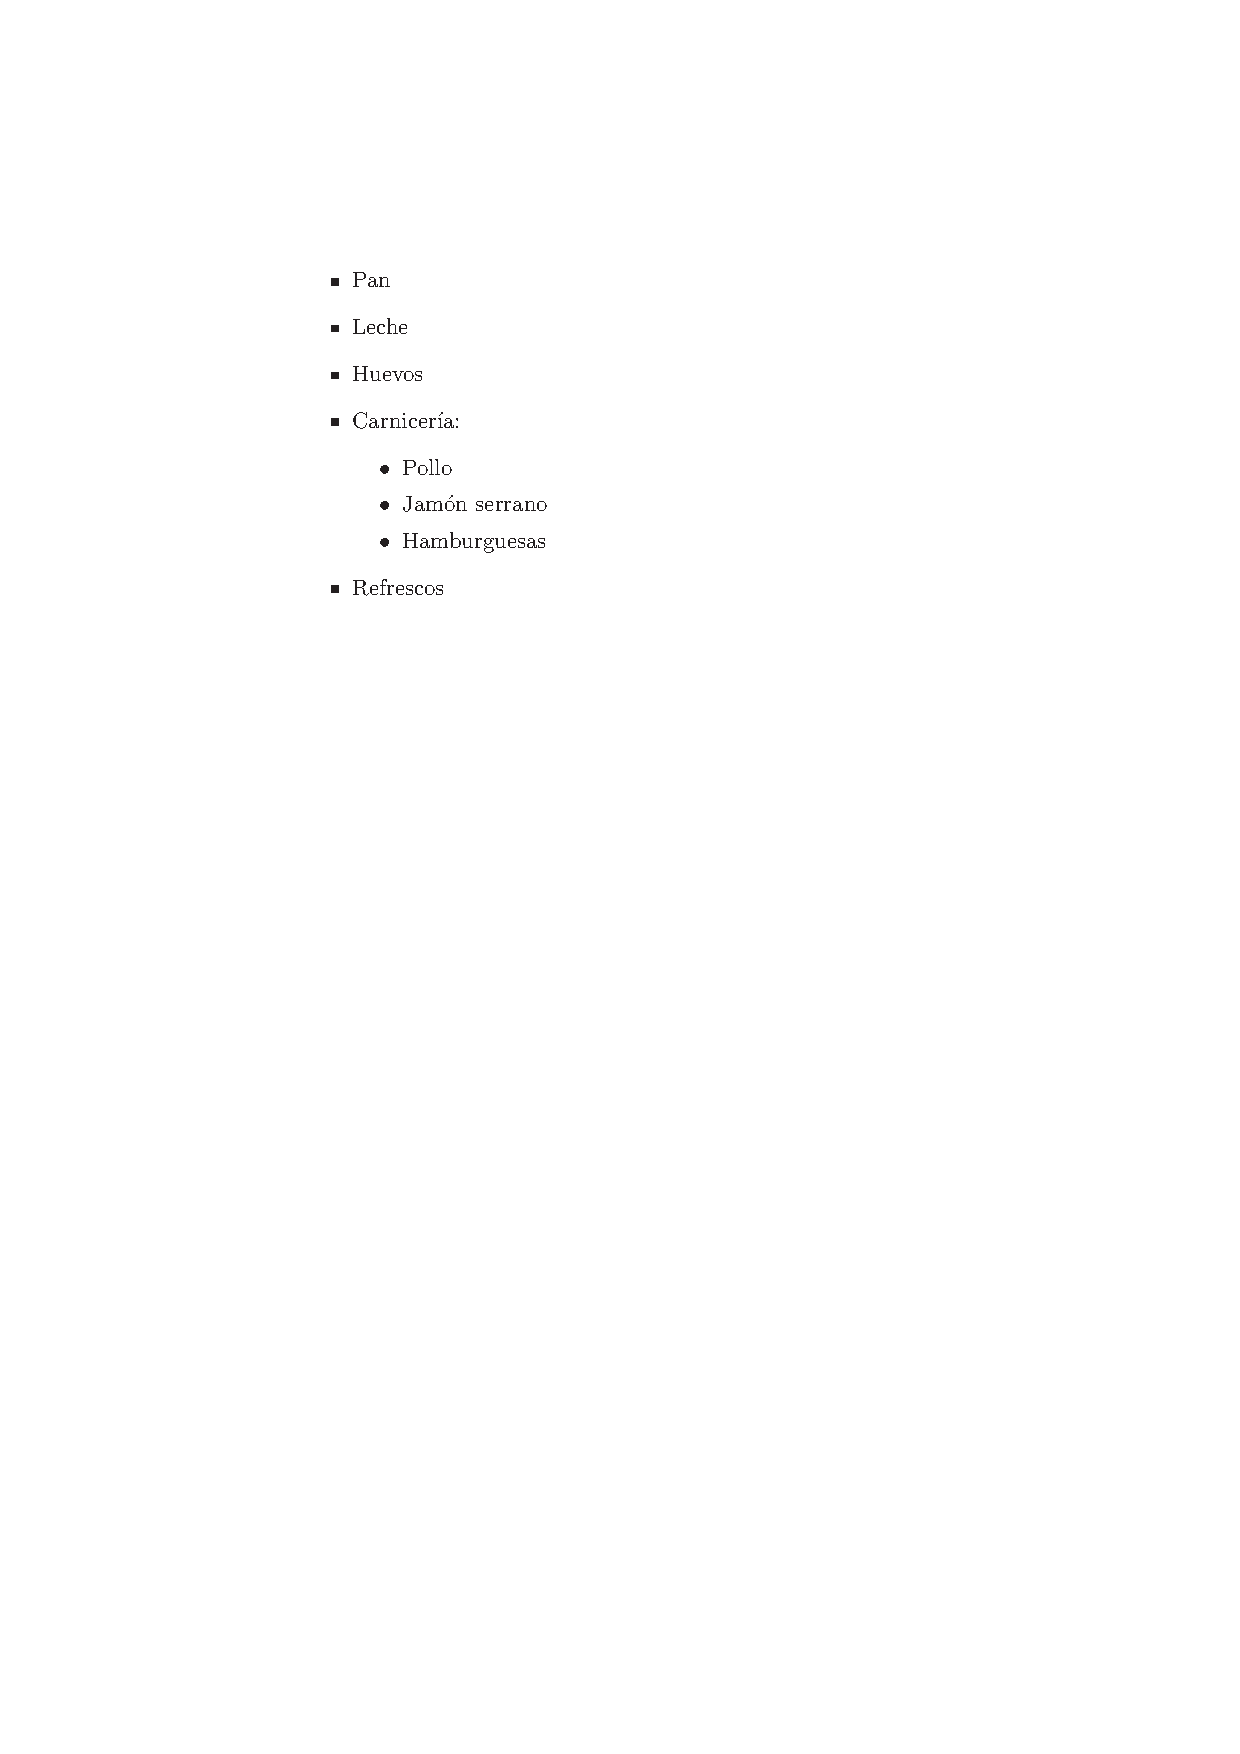
\includegraphics[height=0.4\textheight]{FigurasEjemplos/itemize}};}
{\node[opacity=0.01]{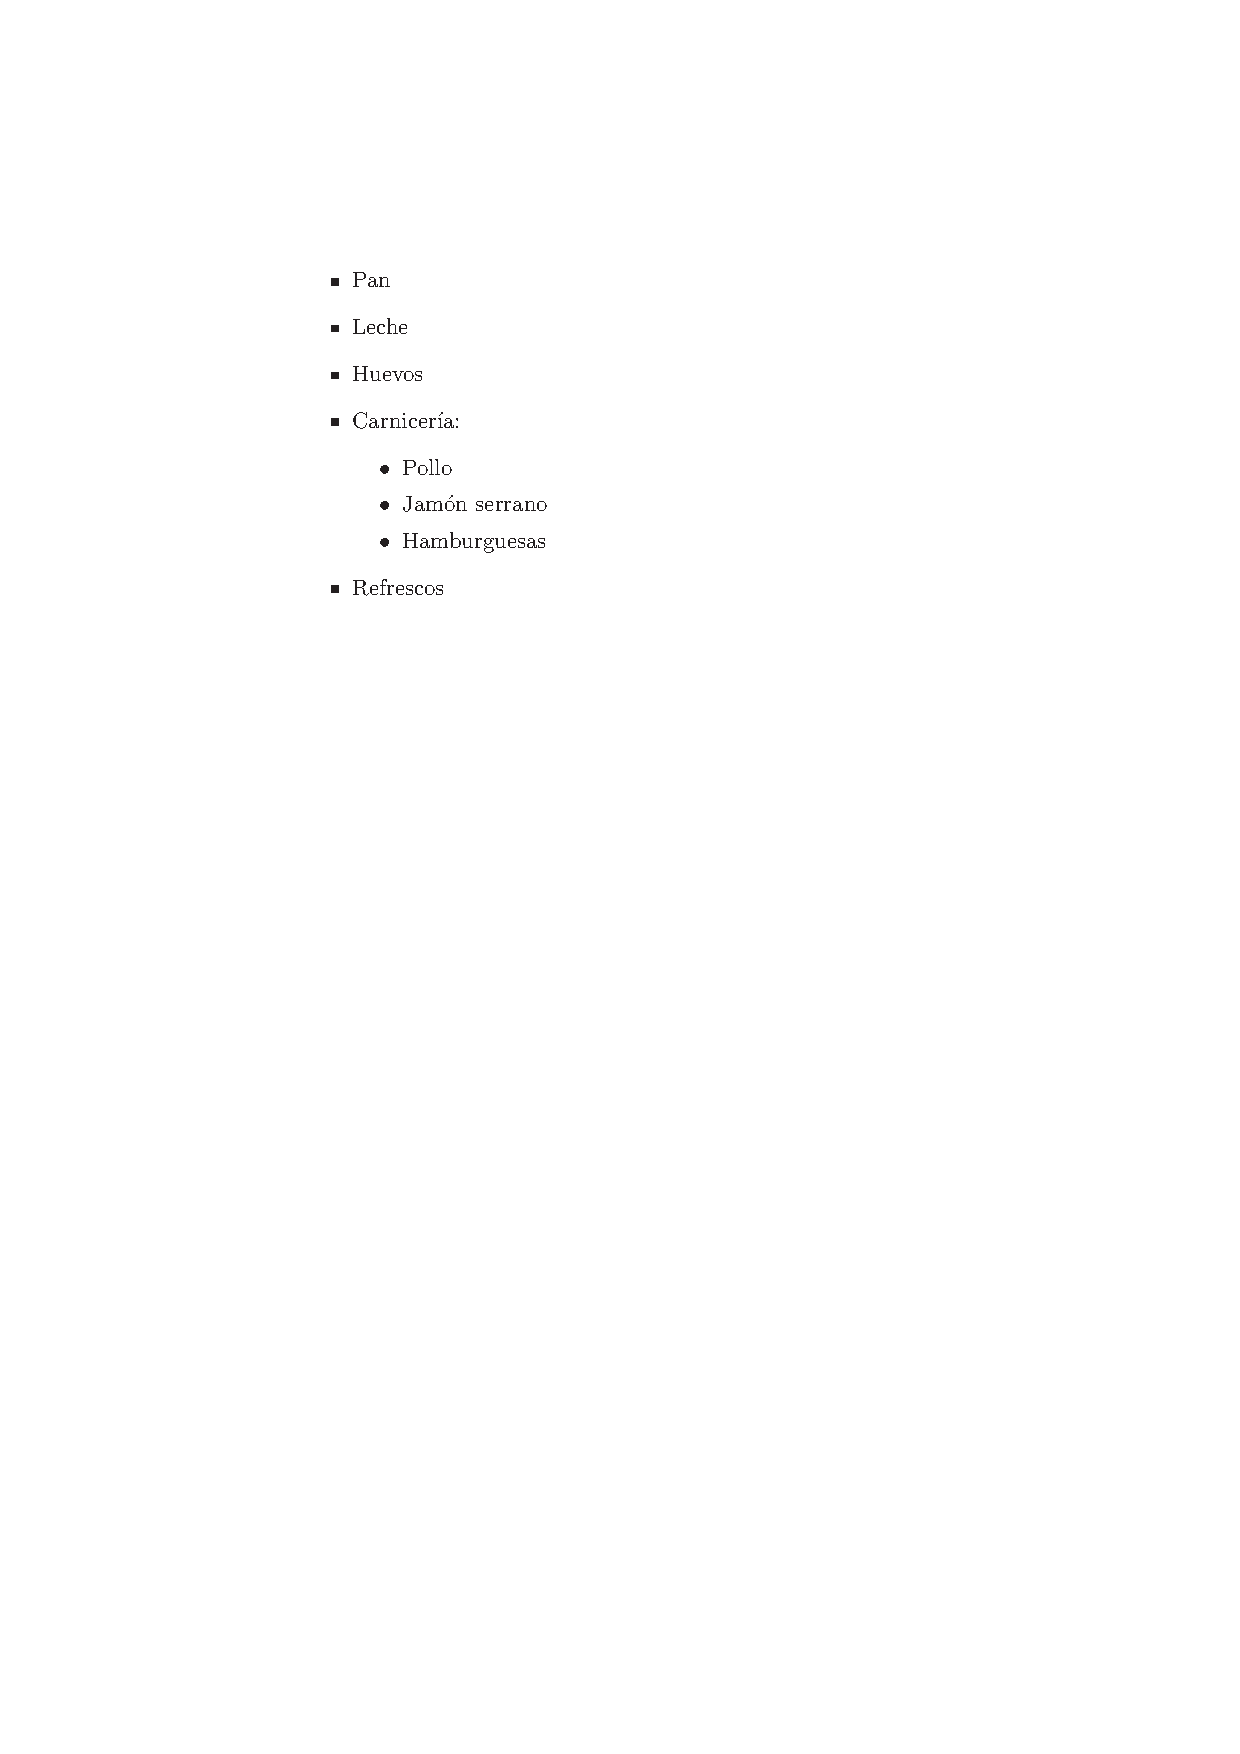
\includegraphics[height=0.4\textheight]{FigurasEjemplos/itemize}};}
\end{tikzpicture}
\end{figure}
\end{minipage}
\hfill
\end{frame}




\begin{frame}[fragile]{Listas numeradas}
\only<1->{
\begin{minipage}{0.65\textwidth}
\begin{itemize}
\item <1->{Los \alert<1->{\textbf<1>{�tems}} se identifican mediante \alert<1->{marcas de orden} (n�meros, letras, \ldots)}

\item <2->{El entorno empleado se denomina \texttt{enumerate}}
\end{itemize}
\end{minipage}}%
\hfill%
\only<3->{
\begin{minipage}{0.3\textwidth}
\begin{sintax}{\texttt{enumerate}}
 \texttt{\backS begin\{enumerate\}}\\
\texttt{\backS item }{\em Texto 1}  \\
\texttt{\backS item }{\em Texto 2}  \\

\vdots

\texttt{\backS end\{enumerate\}}
\end{sintax}
\end{minipage}
}
\pause\pause\pause

\begin{minipage}{0.4\textwidth}
\vspace{-1cm}
\begin{ejem}{\texttt{enumerate}}
\vspace{-0.5cm}
\begin{lstlisting}
\begin{enumerate}
\item Pan
\item Leche
\item Huevos
\item Carnicer�a:
\begin{enumerate}
\item Pollo
\item Jam�n serrano
\item Hamburguesas
\end{enumerate}
\item Refrescos
\end{enumerate}
\end{lstlisting}
\end{ejem}
\end{minipage}%
\pause%
\hspace{1cm}%
\begin{minipage}{0.4\textwidth}
\begin{figure}
\centering
\begin{tikzpicture}
\alt<5->{\node[opacity=1]{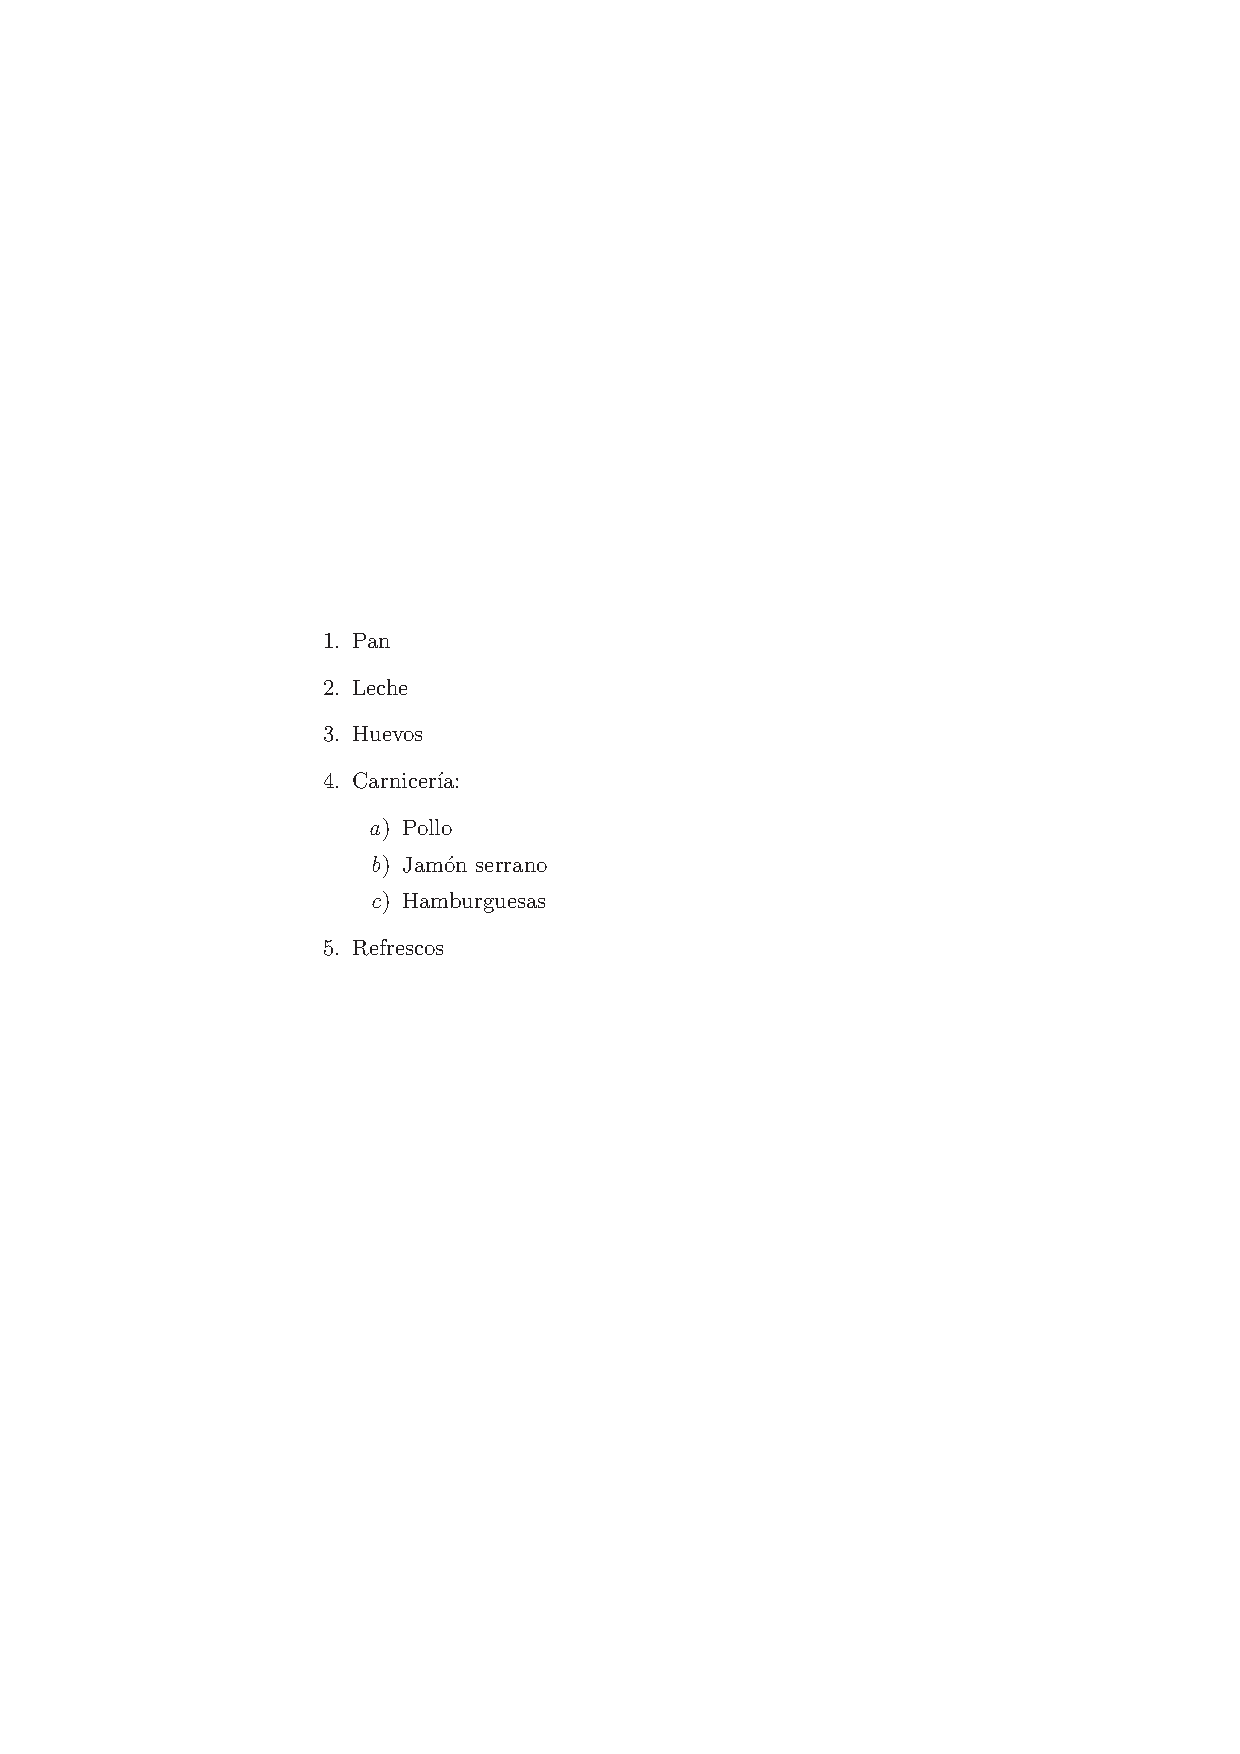
\includegraphics[height=0.4\textheight]{FigurasEjemplos/enumerate}};}
{\node[opacity=0.01]{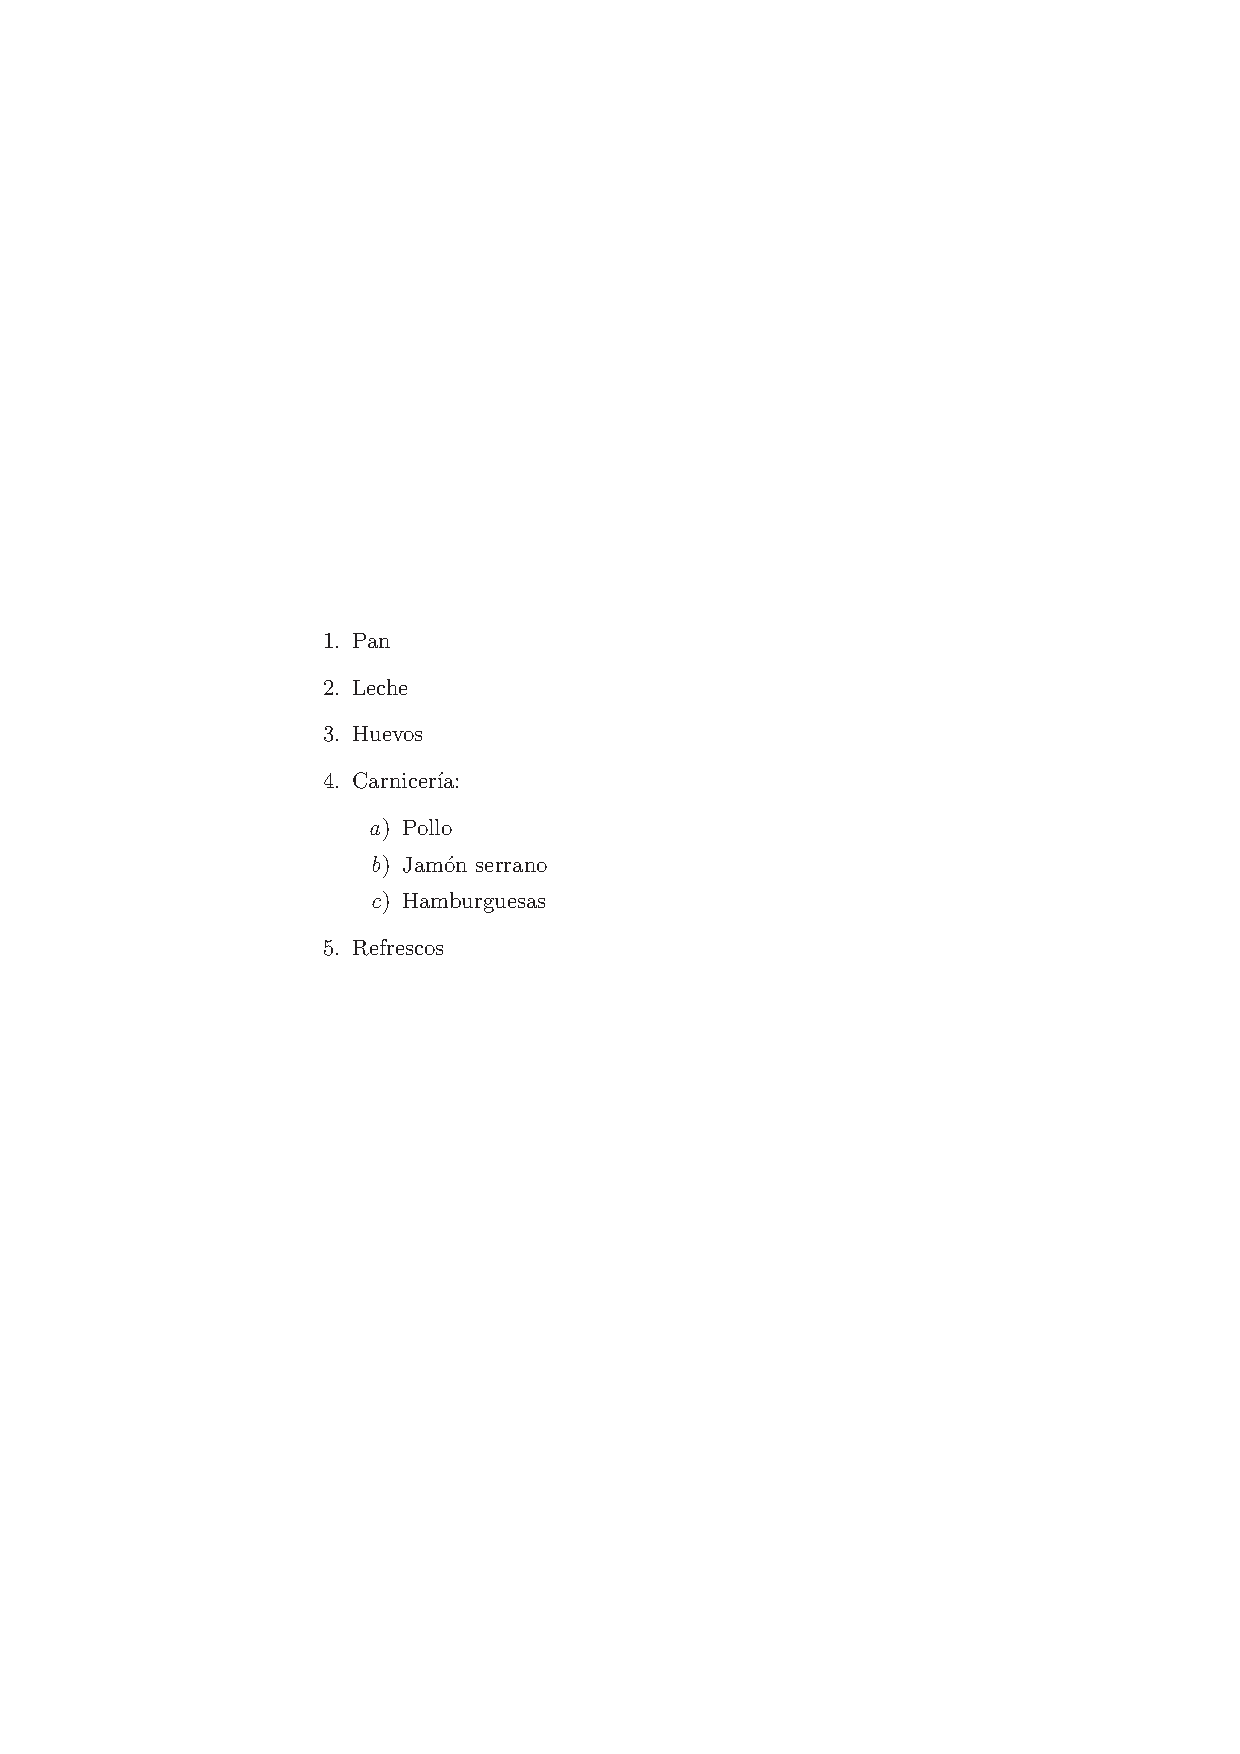
\includegraphics[height=0.4\textheight]{FigurasEjemplos/enumerate}};}
\end{tikzpicture}
\end{figure}
\end{minipage}
\hfill
\end{frame}





\begin{frame}[fragile]{Listas  descriptivas}
\only<1->{
\begin{minipage}{0.6\textwidth}
\begin{itemize}
\item <1->{Los \alert<1->{\textbf<1>{�tems}} son conceptos que se describen}
\item <2->{El entorno empleado se denomina \texttt{description}}
\end{itemize}
\end{minipage}}%
\hfill%
\only<3->{
\begin{minipage}{0.35\textwidth}
\begin{sintax}{\texttt{description}}
 \texttt{\backS begin\{description\}}\\
\texttt{\backS item [{\em etiqueta}]}{\em Texto 1}  \\
\texttt{\backS item  [{\em etiqueta}]}{\em Texto 2}  \\

\vdots

\texttt{\backS end\{description\}}
\end{sintax}
\end{minipage}
}
\pause\pause\pause

\begin{minipage}{0.4\textwidth}
\vspace{-1cm}
\begin{ejem}{\texttt{description}}
\vspace{-0.5cm}
\begin{lstlisting}
\begin{description}
\item [Pan:] comprar en la panader�a
\item [Leche:] comprar en el supermercado
\item [Huevos:] comprar en el supermercado
\item [Carnicer�a:]\hspace{0pt}\par
\begin{itemize}
\item Pollo
\item Jam�n serrano
\item Hamburguesas
\end{itemize}
\item [Refrescos:] comprar en el bazar
\end{description}
\end{lstlisting}
\end{ejem}
\end{minipage}%
\pause%
\hspace{1cm}%
\begin{minipage}{0.4\textwidth}
\begin{figure}
\centering
\begin{tikzpicture}
\alt<5->{\node[opacity=1]{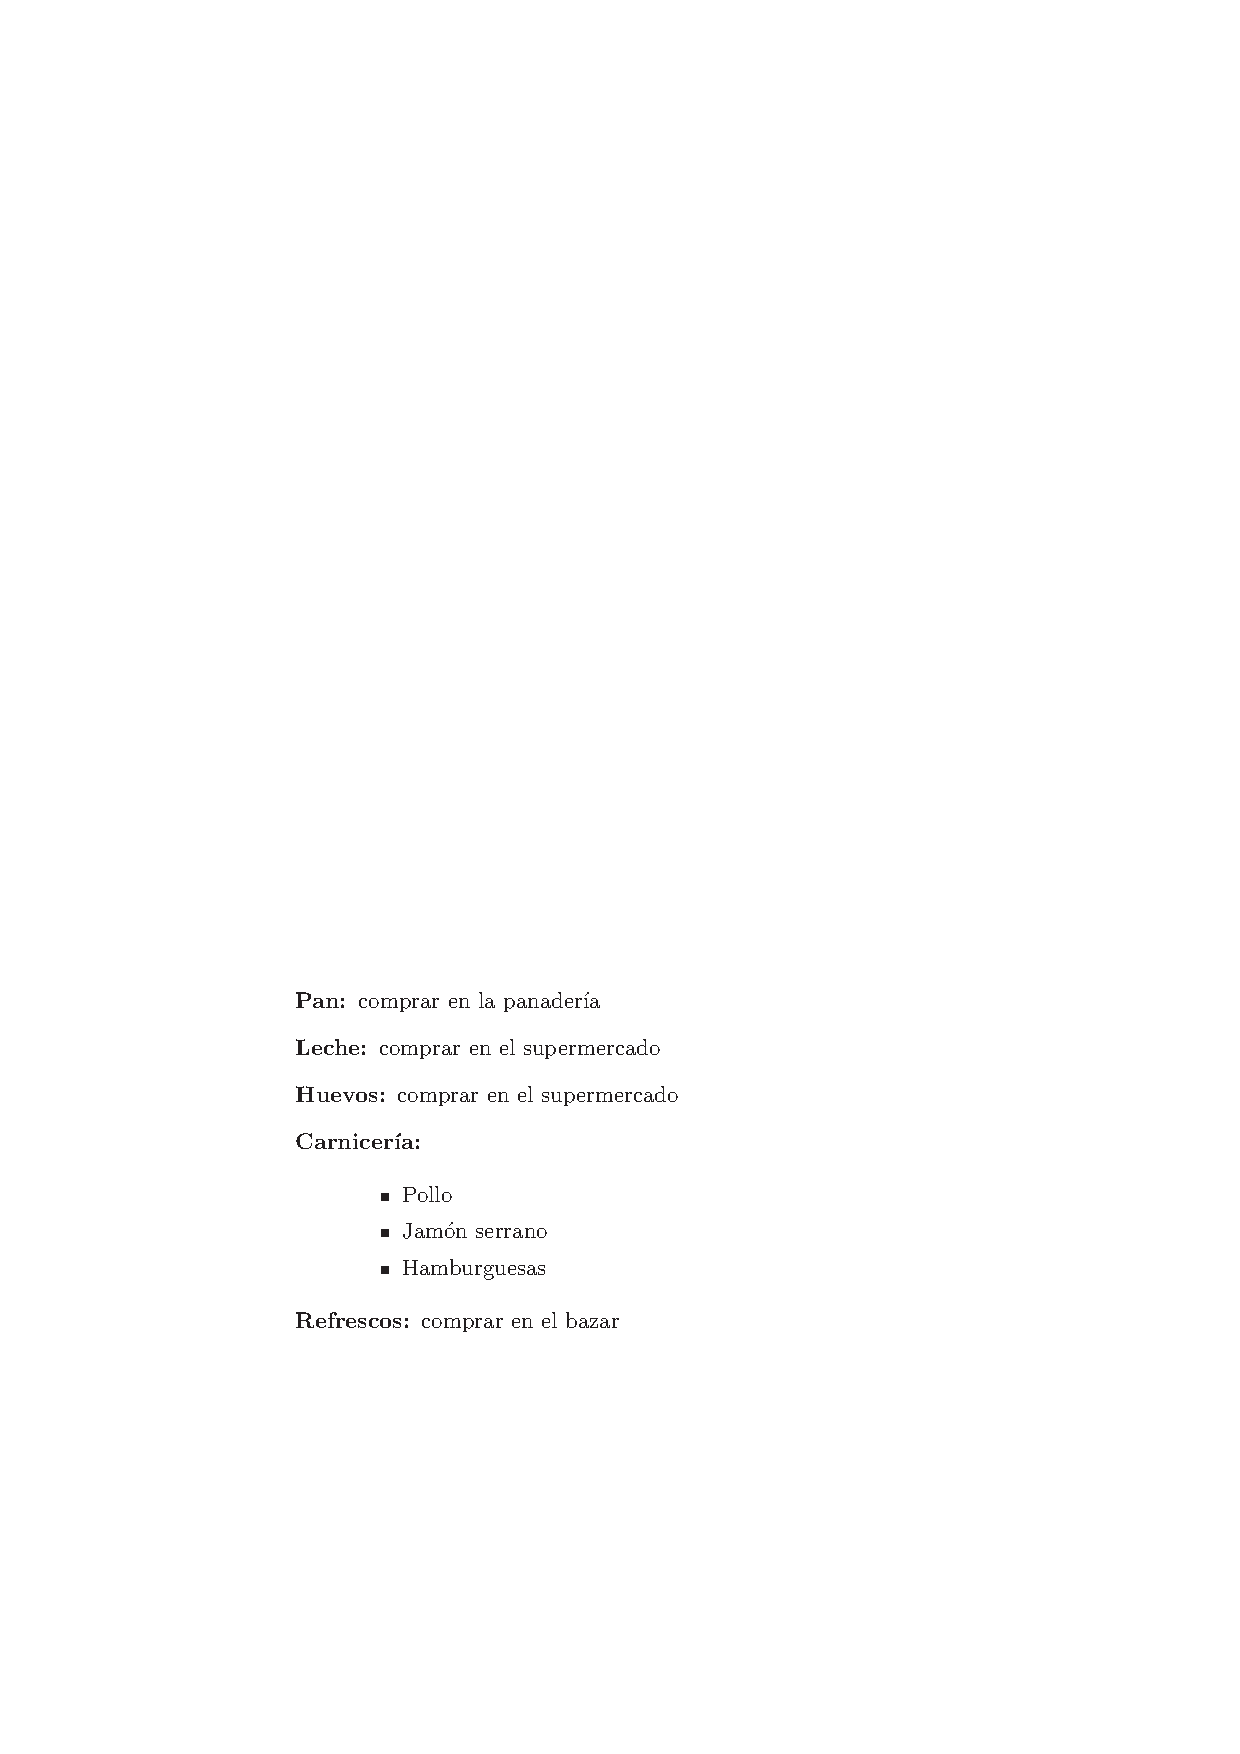
\includegraphics[height=0.4\textheight]{FigurasEjemplos/description}};}
{\node[opacity=0.01]{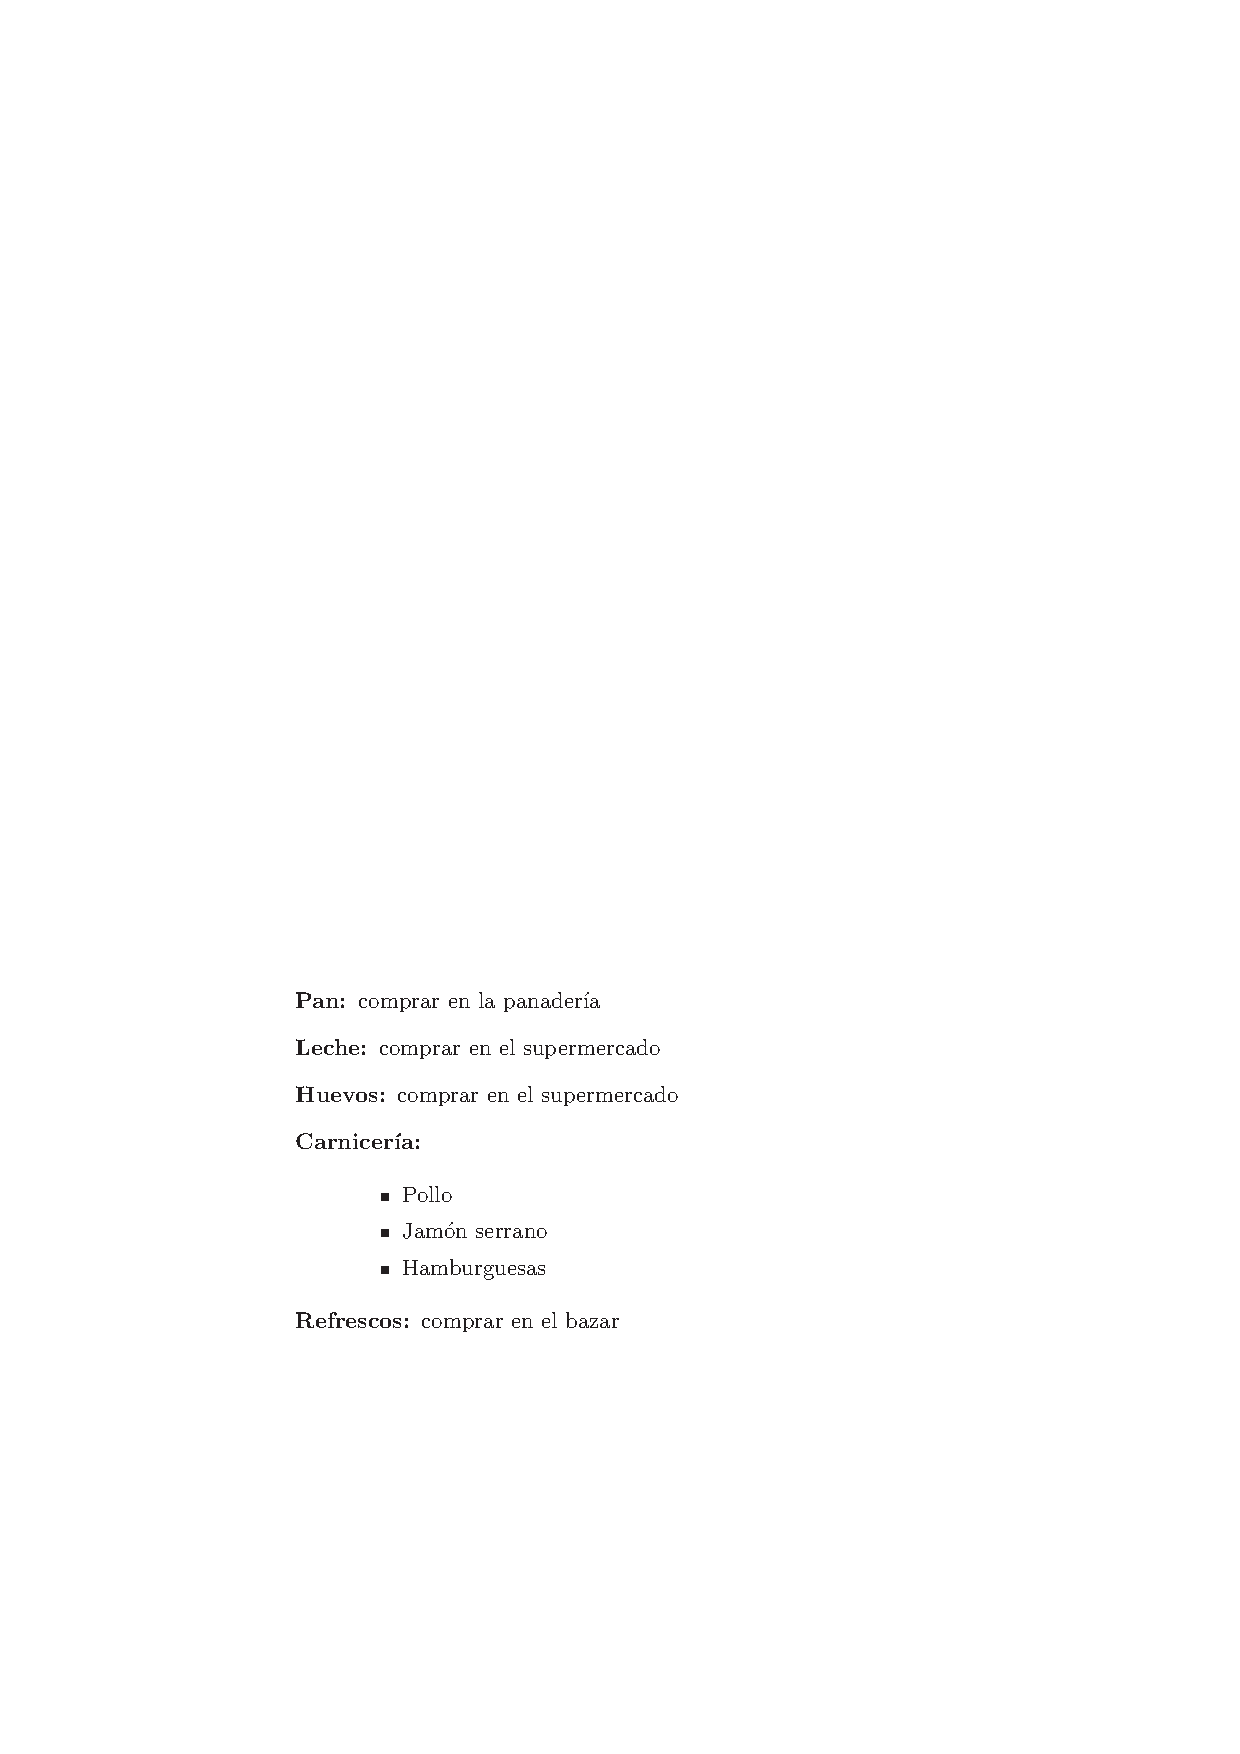
\includegraphics[height=0.4\textheight]{FigurasEjemplos/description}};}
\end{tikzpicture}
\end{figure}
\end{minipage}
\hfill
\end{frame}





\subsection{Notas}


\begin{frame}[fragile]{Las notas al pie de p�gina}

\begin{itemize}
\item <1->Las notas son advertencias, explicaciones o comentarios que se sit�an fuera del texto general
\item <2->Se introducen mediante una marca (v.g. cifra o letra)
\end{itemize}
\only<3->{
\begin{sintax}{\texttt{\backS footnote}}
\texttt{\backS footnote[n�mero\only<4>{ \alert<4>{(opcional)}}]\{{\em Texto de la nota}\}}
\end{sintax}}

\pause\pause\pause\pause
\begin{minipage}{0.6\textwidth}
\begin{ejem}{\texttt{\backS footnote}}
\vspace{-0.5cm}
\begin{lstlisting}
Este texto tiene dos notas\footnote{Esta es la primera nota} al pie de p�gina que, gracias a \LaTeX{}, se numeran solas\footnote{Esta es la segunda nota}.
\end{lstlisting}
\end{ejem}
\end{minipage}%
\pause%
\hfill%
\begin{minipage}{0.39\textwidth}
\begin{figure}
\centering
\begin{tikzpicture}
\alt<5->{\node[opacity=1]{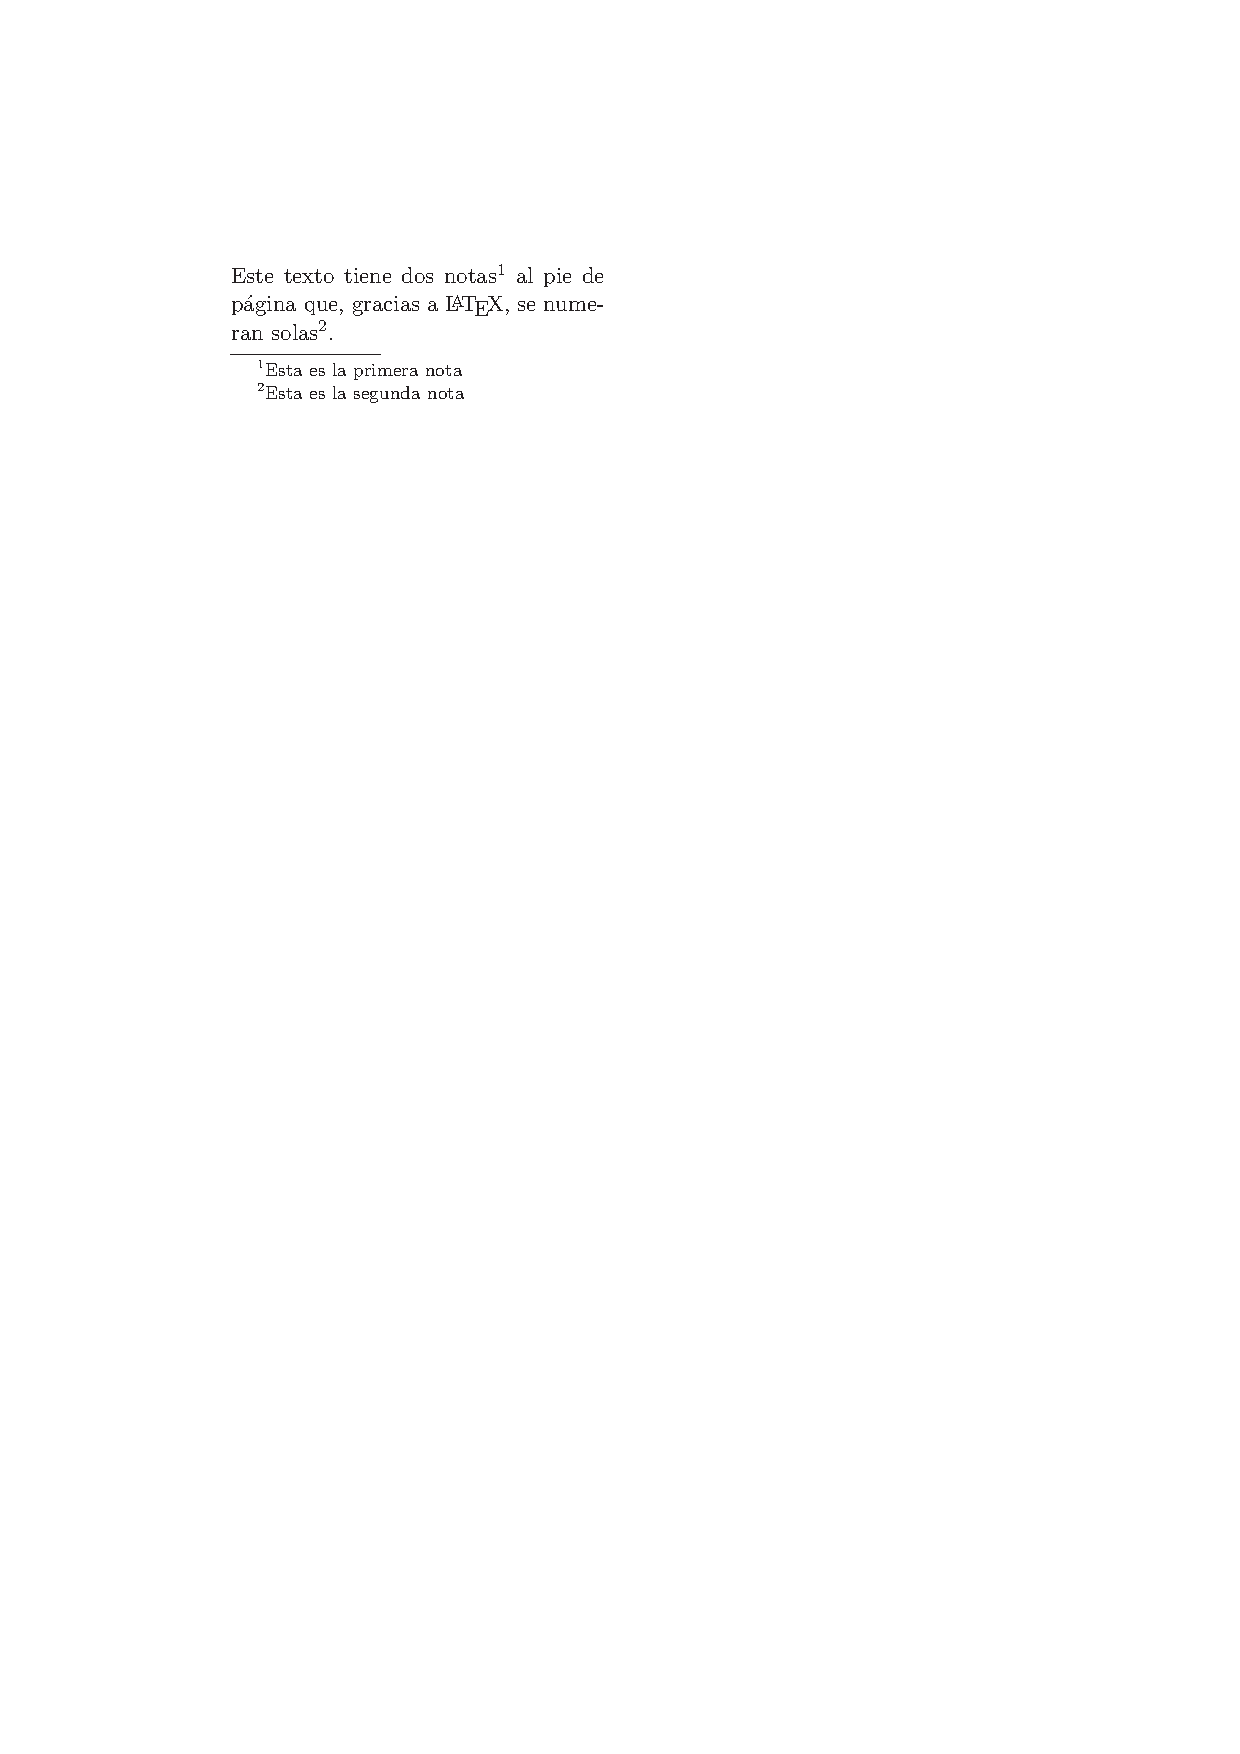
\includegraphics[width=\textwidth]{FigurasEjemplos/footnote}};}
{\node[opacity=0.01]{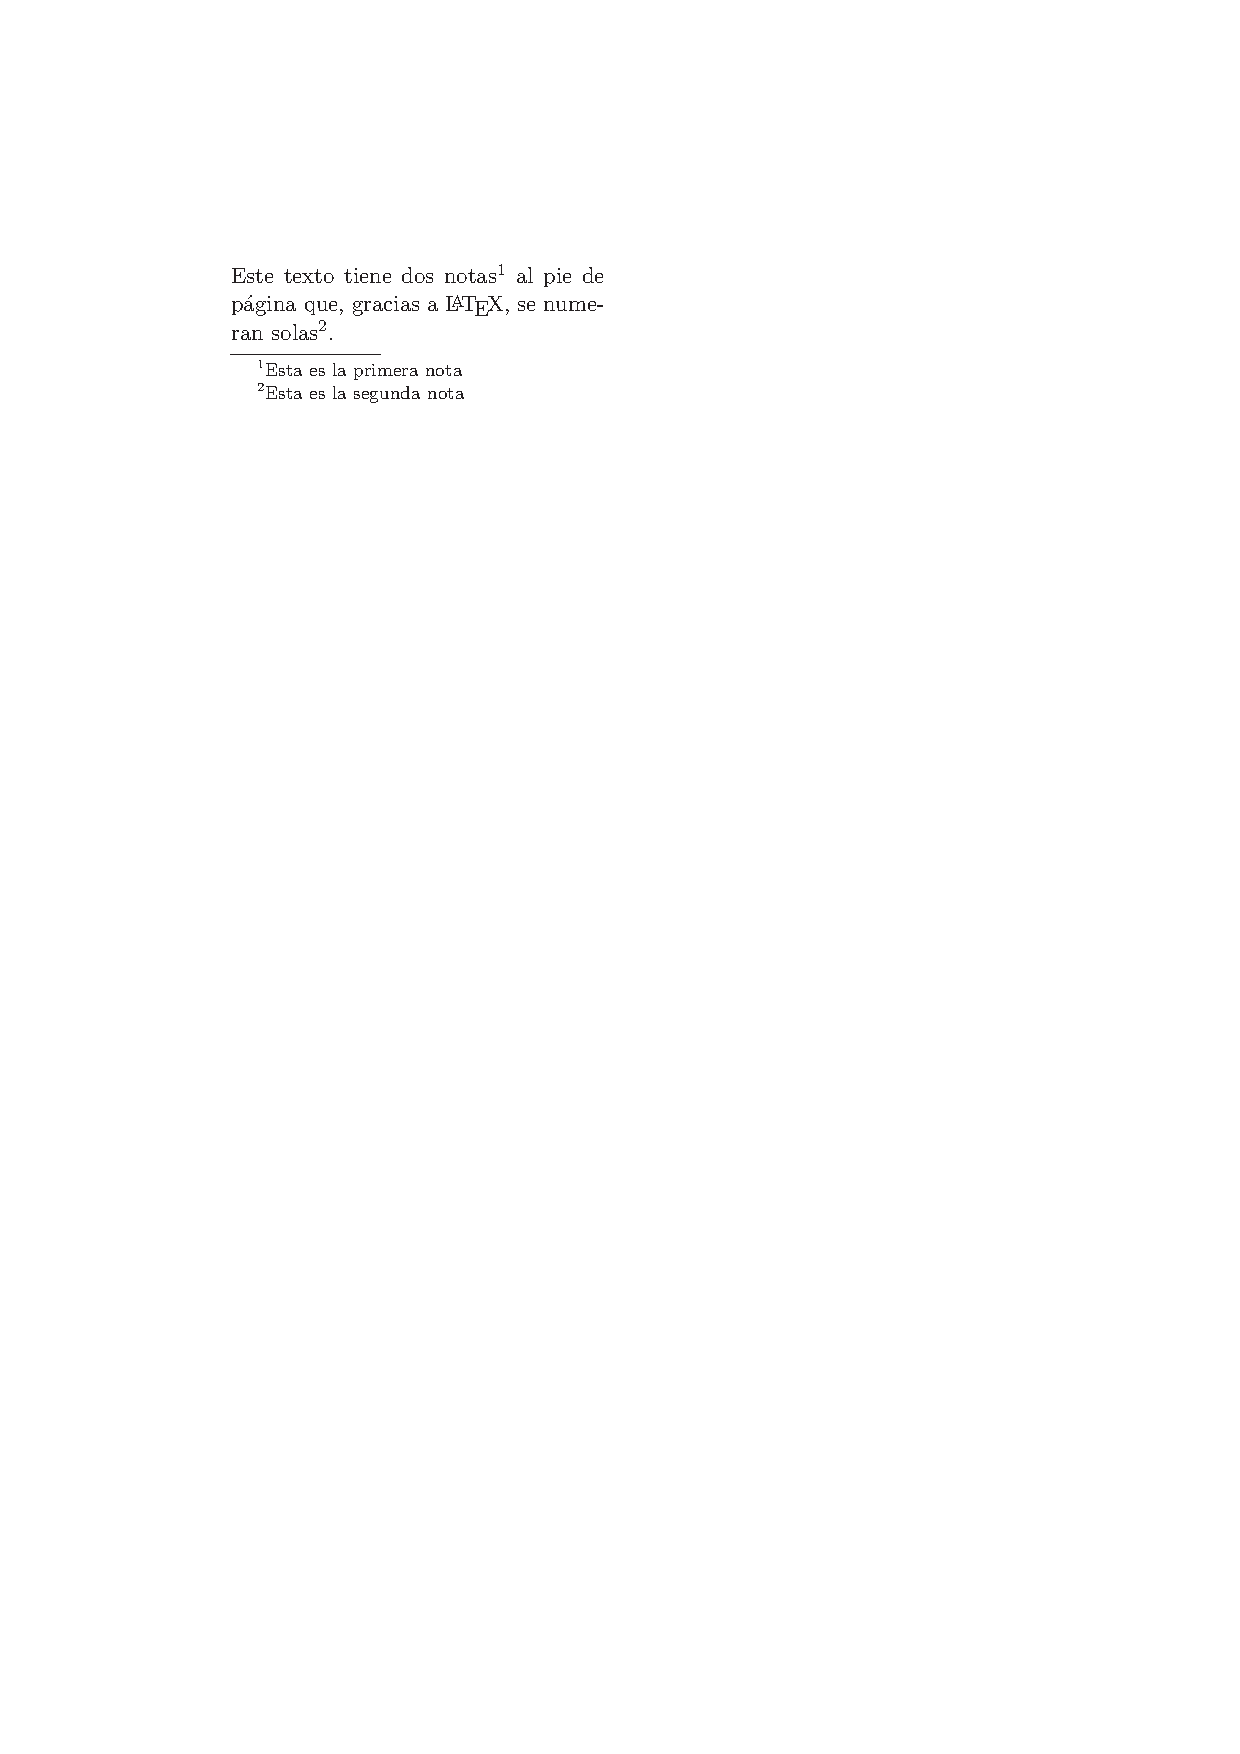
\includegraphics[width=\textwidth]{FigurasEjemplos/footnote}};}
\end{tikzpicture}
\end{figure}
\end{minipage}

\end{frame}


\subsection{Alineaci�n del texto}


\begin{frame}[fragile]{Alineaci�n del texto}

\begin{itemize}
\item <1->Normalmente alineamos a la izquierda, a la derecha o al centro
\item <2->\LaTeX{} se encarga de \alert<2>{justificar} el texto autom�ticamente
\item <3->Los entornos son: \texttt{flushright} (dcha.), \texttt{flushleft} (izq.), \texttt{center} (centro)
\end{itemize}
\begin{center}
\only<4->{
\begin{minipage}{0.3\textwidth}
\begin{sintax}{\texttt{flushright}}
\texttt{\backS begin\{flushright\}}\\
{\it Texto}\\
\texttt{\backS end\{flushright\}}
\end{sintax}
\end{minipage}}%
\hspace{1cm}
\only<5->{
\begin{minipage}{0.3\textwidth}
\begin{sintax}{\texttt{flushleft}}
\texttt{\backS begin\{flushleft\}}\\
{\it Texto}\\
\texttt{\backS end\{flushleft\}}
\end{sintax}
\end{minipage}}%
\end{center}
\only<6->{
\begin{center}
\begin{minipage}{0.3\textwidth}
\begin{sintax}{\texttt{center}}
\texttt{\backS begin\{center\}}\\
{\it Texto}\\
\texttt{\backS end\{center\}}
\end{sintax}
\end{minipage}
\end{center}}

\end{frame}


\subsection{Tablas}


\begin{frame}[fragile]{Las tablas (I)}

\begin{itemize}
\item <1->Son un elemento {\color{red}{\bf delicado}} en \LaTeX{}: no son sencillas de construir
\item <2-> Son muy {\color{miverdeO}{\bf flexibles}}
\item <3-> Existen {\color{miverdeO}complementos} que vinculan \LaTeX{} y {\color{miverdeO}Excel} \only<4>{\bien}
\item <5-> El entorno empleado es \texttt{tabular}
\end{itemize}
\only<6->{
\begin{sintax}{\texttt{tabular}}
\texttt{\backS begin\{tabular\}[{\em posicion}]\{{\em formato columnas}\}}\\
$elem_{11}$ \texttt{\&} $elem_{12}$ \texttt{\&} \ldots  \texttt{\&} $elem_{1m}$ \backS\backS\\
$elem_{11}$ \texttt{\&} $elem_{22}$ \texttt{\&} \ldots  \texttt{\&} $elem_{2m}$ \backS\backS\\
\vdots

$elem_{n1}$ \texttt{\&} $elem_{n2}$ \texttt{\&} \ldots  \texttt{\&} $elem_{nm}$ \backS\backS\\
\texttt{\backS end\{tabular\}}
\end{sintax}}
\end{frame}


\begin{frame}[fragile]{Las tablas (II)}
\vspace{-0.3cm}
\begin{minipage}{0.5\textwidth}
\begin{ejem}{\texttt{tabular}}
\vspace{-0.5cm}
\begin{lstlisting}
\begin{tabular}{lccc}
      Pa�s &      Total &     Perros &      Gatos \\
    Espa�a &       3000 &       1600 &       1400 \\
    Angola &       5000 &       3000 &       2000 \\
   Hungr�a &       3200 &       2800 &        400 \\
      Per� &       1300 &        400 &        900 \\
\end{tabular}
\end{lstlisting}
\end{ejem}
\end{minipage}%
\pause%
\hfill%
\begin{minipage}{0.39\textwidth}
\vspace{0.15cm}
\begin{figure}
\centering
\begin{tikzpicture}
\alt<2->{\node[opacity=1]{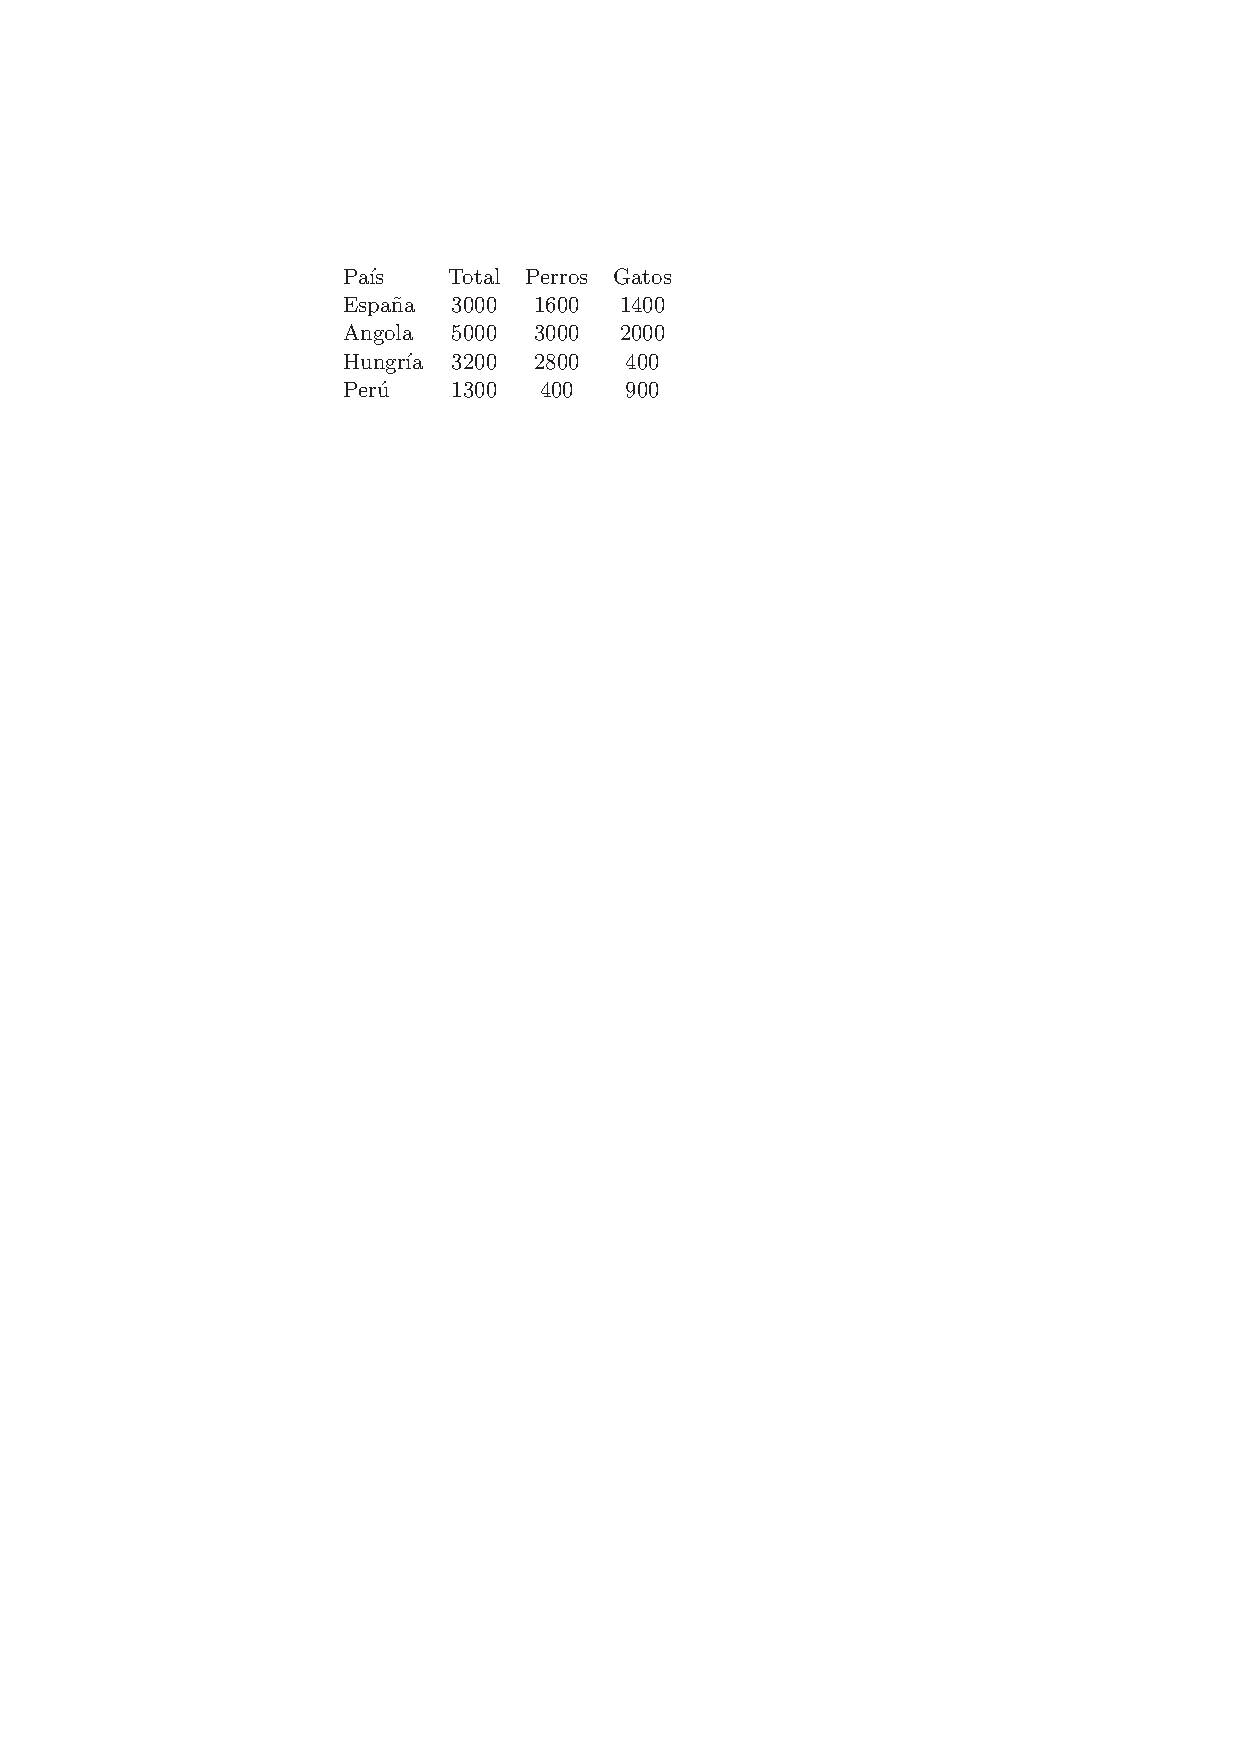
\includegraphics[width=\textwidth]{FigurasEjemplos/tabular}};}
{\node[opacity=0.01]{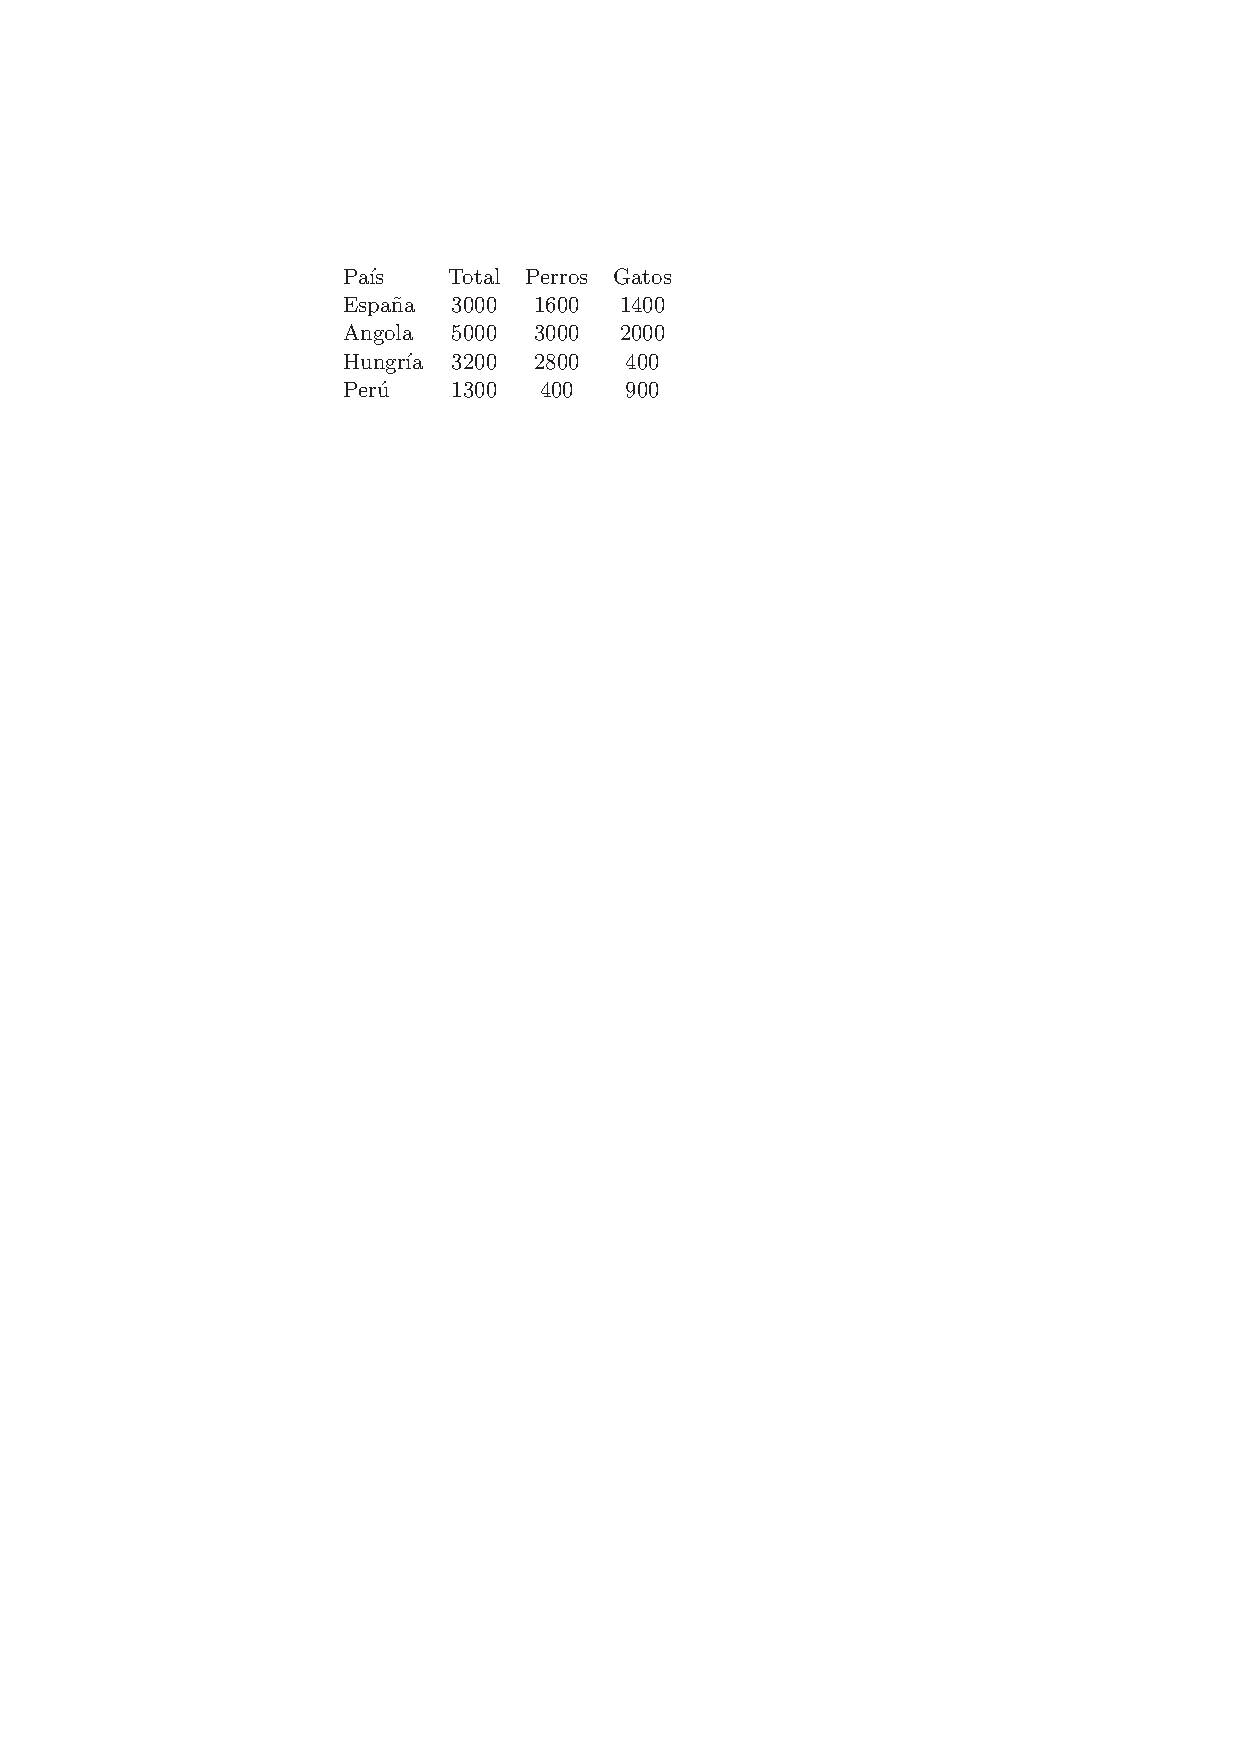
\includegraphics[width=\textwidth]{FigurasEjemplos/tabular}};}
\end{tikzpicture}
\end{figure}
\end{minipage}

\pause
\begin{minipage}{0.5\textwidth}
\vspace{-0.2cm}
\begin{ejem}{\texttt{tabular}}
\vspace{-0.5cm}
\begin{lstlisting}
\begin{tabular}{|l|c|c|c|}
\hline
      Pa�s &      Total &     Perros &      Gatos \\
\hline
    Espa�a &       3000 &       1600 &       1400 \\
\hline
    Angola &       5000 &       3000 &       2000 \\
\hline
   Hungr�a &       3200 &       2800 &        400 \\
\hline
      Per� &       1300 &        400 &        900 \\
\hline
\end{tabular}  
\end{lstlisting}
\end{ejem}
\end{minipage}%
\pause%
\hfill%
\begin{minipage}{0.39\textwidth}
\begin{figure}
\centering
\begin{tikzpicture}
\alt<4->{\node[opacity=1]{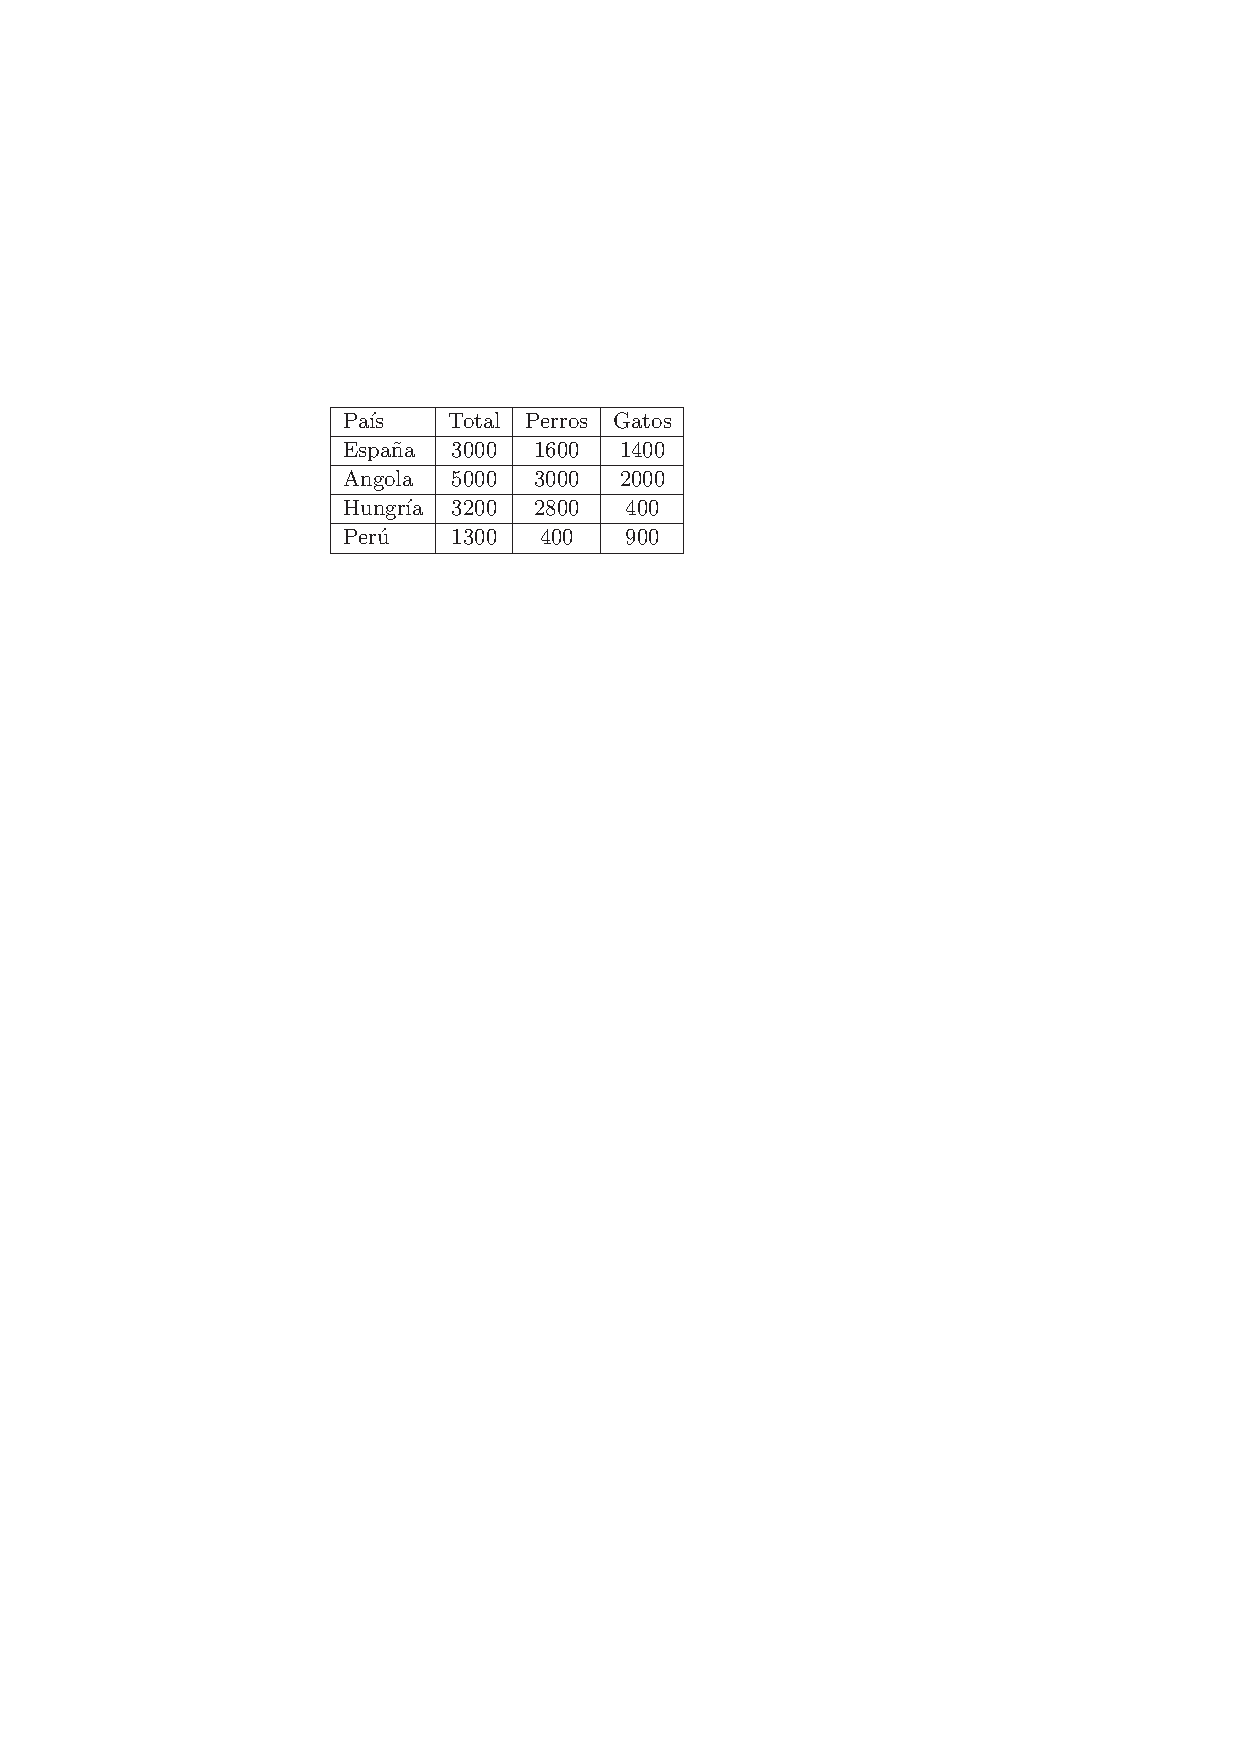
\includegraphics[width=\textwidth]{FigurasEjemplos/tabular2}};}
{\node[opacity=0.01]{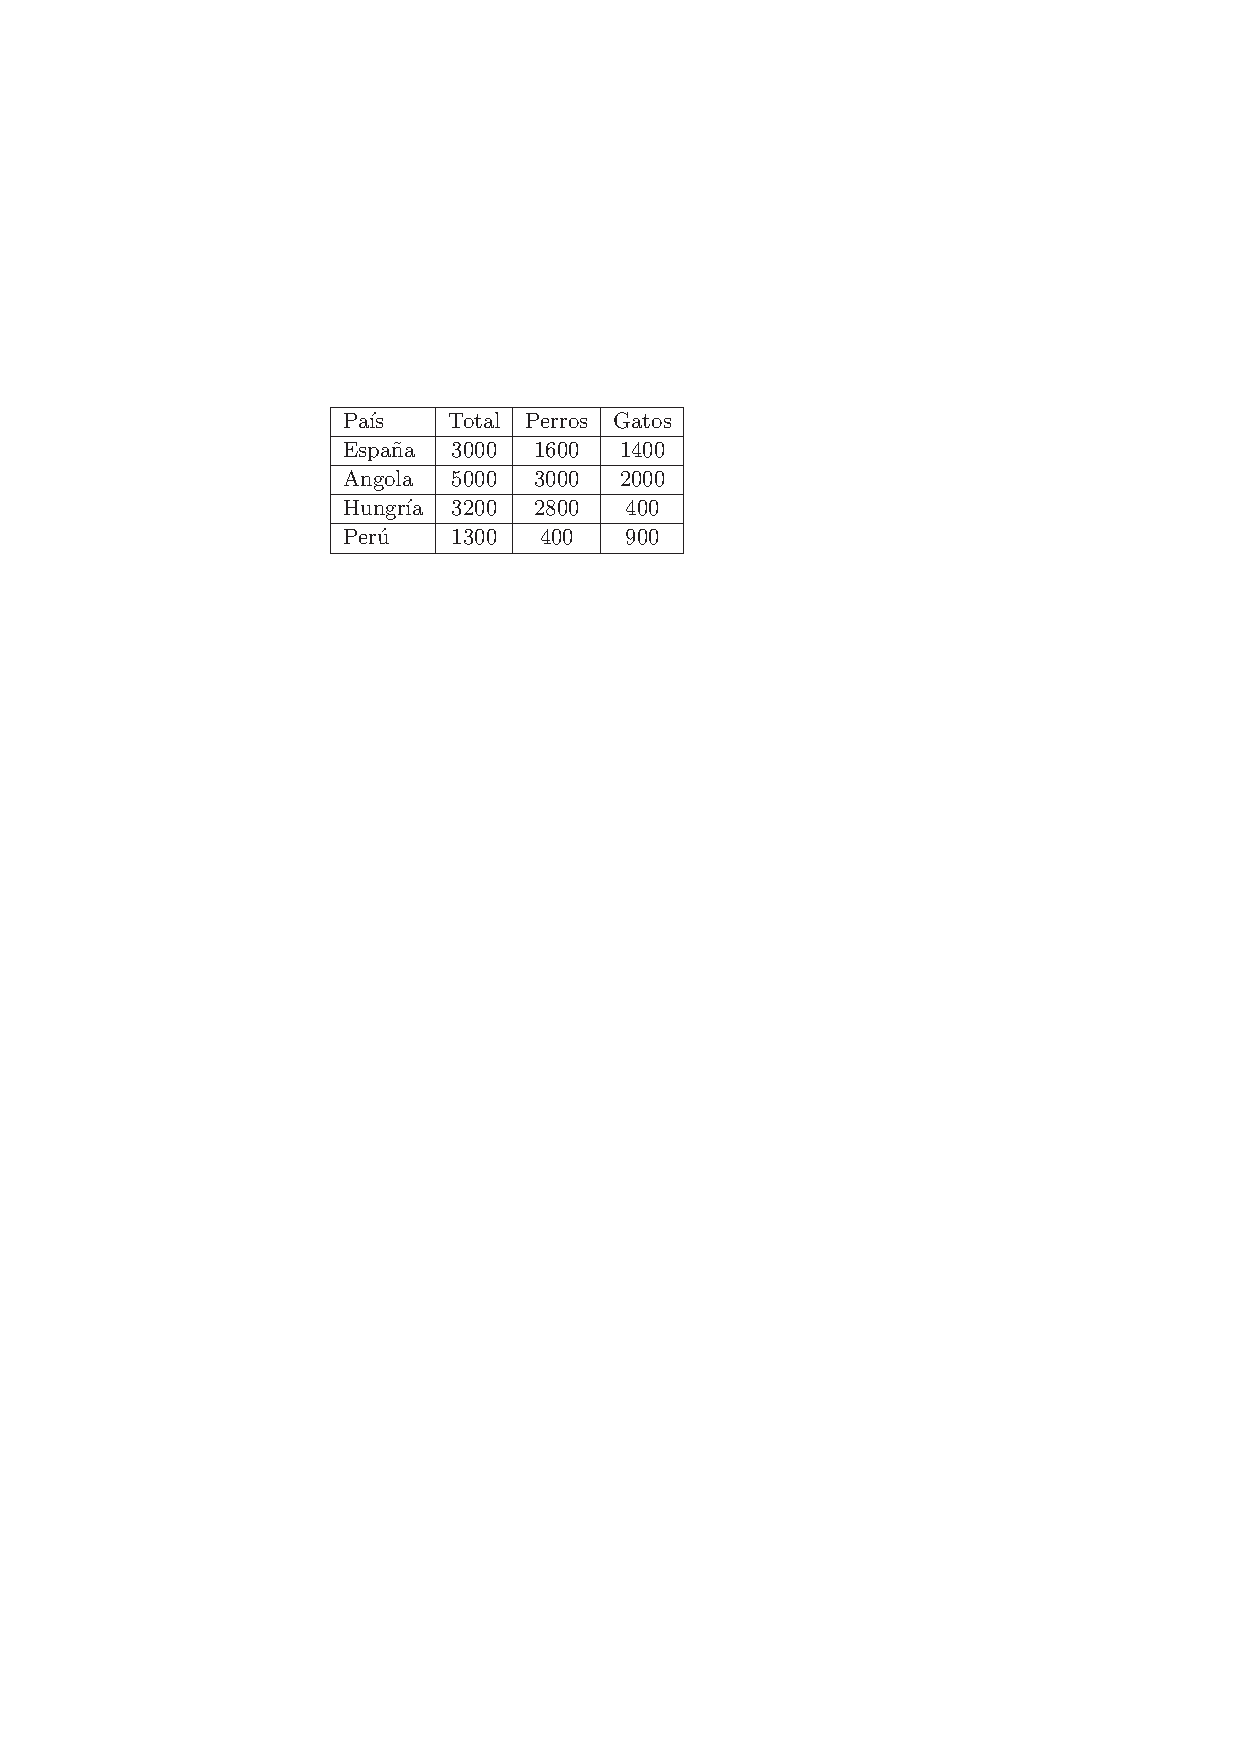
\includegraphics[width=\textwidth]{FigurasEjemplos/tabular2}};}
\end{tikzpicture}
\end{figure}
\end{minipage}

\end{frame}








\subsection{�Manos a la obra!}

\begin{frame}[fragile]{Nuestro ejemplo: Report }
\vspace{-0.1cm}
\begin{center}
\only<1>{
Vamos a a�adir, entre el final de la {\bf subsecci�n 1.1.2} y el {\bf Ap�ndice A} otra secci�n con todo lo aprendido en este cap�tulo.}
\only<2->{
\begin{minipage}{0.32\textwidth}
\begin{figure}[hbtp]
\centering
\fbox{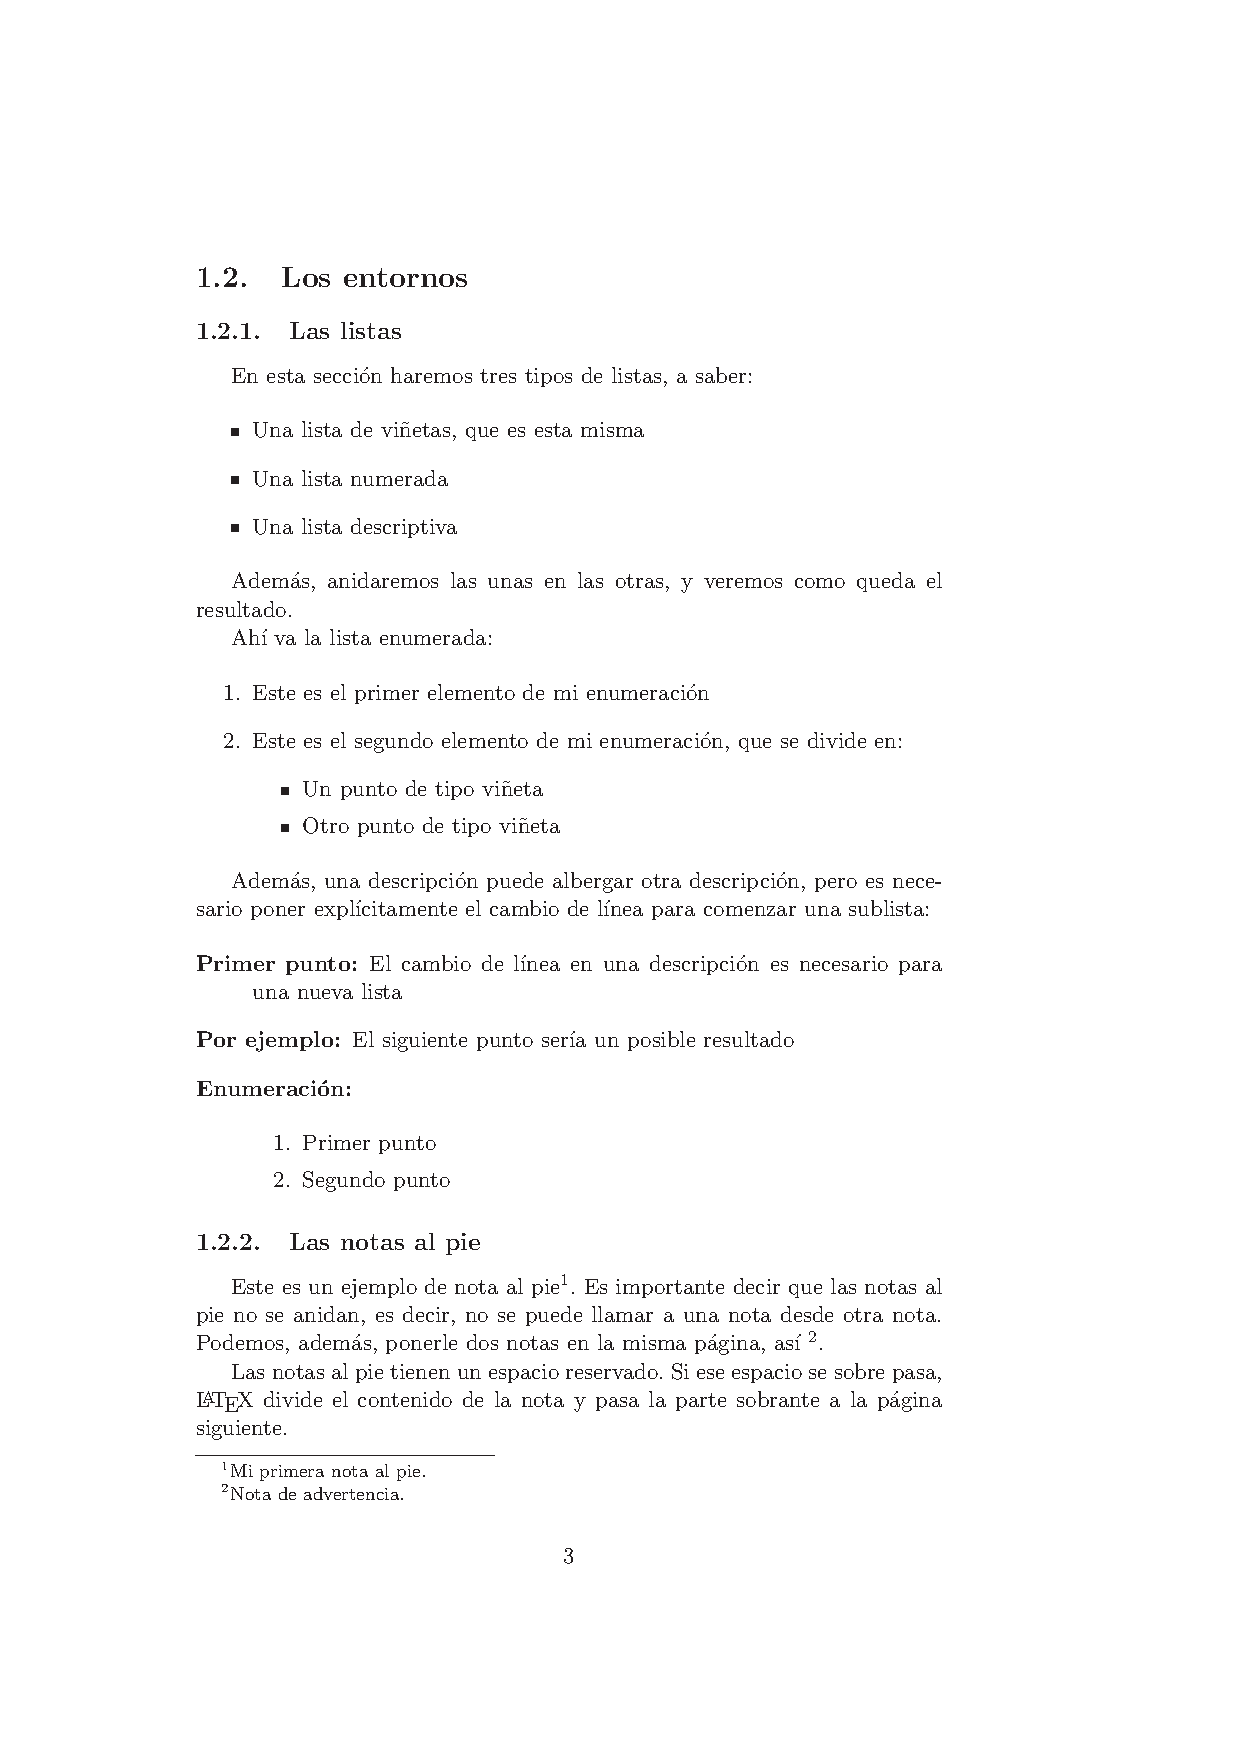
\includegraphics[width=\textwidth, page=1]{FigurasEjemplos/Ejercicio3}}
\end{figure}
\end{minipage}%
\hspace{1cm}
\begin{minipage}{0.32\textwidth}
\begin{figure}[hbtp]
\centering
\fbox{\includegraphics[width=\textwidth, page=2]{FigurasEjemplos/Ejercicio3}}
\end{figure}
\end{minipage}}
\end{center}
\end{frame}

\begin{frame}[fragile]{Nuestro ejemplo: Report}
\vspace{-0.5cm}
\begin{lstlisting}
\newpage %Para  cambiar de p�gina
\section{Los entornos}
\subsection{Las listas}
En esta secci�n haremos tres tipos de listas, a saber:
\begin{itemize}
\item Una lista de vi�etas, que es esta misma
\item Una lista numerada
\item Una lista descriptiva
\end{itemize}
Adem�s, anidaremos las unas en las otras, y veremos como queda el resultado.\\%cambio de linea
Ah� va la lista enumerada:
\begin{enumerate}
\item Este es el primer elemento de mi enumeraci�n
\item Este es el segundo elemento de mi enumeraci�n, que se divide en:
\begin{itemize}
\item Un punto de tipo vi�eta
\item Otro punto de tipo vi�eta
\end{itemize}
\end{enumerate}
Adem�s, una descripci�n puede albergar otra descripci�n, pero es necesario poner expl�citamente el cambio de l�nea para comenzar una sublista:
\begin{description}
\item [Primer punto:] El cambio de l�nea en una descripci�n es necesario para una nueva lista
\item [Por ejemplo:] El siguiente punto ser�a un posible resultado
\item [Enumeraci�n:]\hspace{0pt}\par
\begin{enumerate}
\item Primer punto
\item Segundo punto
\end{enumerate}
\end{description}
\end{lstlisting}%

\end{frame}

\begin{frame}[fragile]{Nuestro ejemplo: Report}
\vspace{-0.5cm}
\begin{lstlisting}
\subsection{Las notas al pie}
Este es un ejemplo de nota al pie\footnote{Mi primera nota al pie.}. Es importante decir que las notas al pie no se anidan, es decir, no se puede llamar a una nota desde otra nota. Podemos, adem�s, ponerle dos notas en la misma p�gina, as� \footnote{Nota de advertencia.}.\\
Las notas al pie tienen un espacio reservado. Si ese espacio se sobre pasa, \LaTeX{} divide el contenido de la nota y pasa la parte sobrante a la p�gina siguiente.
\subsection{La justificaci�n}
Aqu� pondremos en pr�ctica la justificaci�n del texto. Por ejemplo:
\begin{flushright}
Este texto est� justificado a la derecha
\end{flushright}
\begin{flushleft}
Este texto est� justificado a la izquierda
\end{flushleft}
\begin{center}
Este texto est� muy bien centradito 
\end{center}

\subsection{Las tablas}
Escribiremos en esta subsecci�n lo que hemos aprendido respecto a las tablas en el cap�tulo {\sc entornos} de \cite{Cabrero}.
\begin{center}
\begin{tabular}{||l|c|r||}
\hline
\end{lstlisting}%

\end{frame}


\begin{frame}[fragile]{Nuestro ejemplo: Report}
\vspace{-0.5cm}
\begin{lstlisting}
{\bf Nombre} & {\bf Apellido} & {\bf Rol} \\
\hline\hline
Pepito & P�rez & Estudiante \\
\hline
Jorge & Garc�a & Estudiante \\
\hline
Mar�a & Pi�ales & Profesor \\
\hline
Olga & Roca & Administraci�n \\
\hline
\end{tabular}
\end{center}
Por otra parte, si queremos hacer una casillla multicolumna, emplearemos el comando {\tt \textbackslash multicolumn\{{\em n�mero columnas}\}\{{\em justificaci�n}\}}\{{\em Texto}\}, y quedar� el siguiente resultado (que se ha justificado a la derecha):
\begin{flushright}
\begin{tabular}{||l|c|r||}
\hline
\multicolumn{2}{||l|}{\bf Nombre Completo} & {\bf Rol} \\
\hline\hline
Pepito & P�rez & Estudiante \\
\hline
Jorge & Garc�a & Estudiante \\
\hline
Mar�a & Pi�ales & Profesor \\
\hline
Olga & Roca & Administraci�n \\
\hline
\end{tabular}
\end{flushright}
\end{lstlisting}%

\end{frame}



\section{Personalizaci�n}

%----------------------------------------%----------------------------------------%----------------------------------------
\subsection{Tipos de letra}

\begin{frame}{Introducci�n}
\begin{itemize}
\item <1-> Los tipos que por defecto emplea \LaTeX{} los cre� Knuth para \TeX{}
\item <2-> Los denomin� {\bf Computer Modern Fonts}
\item <3-> No obstante, se pueden emplear otros tipos
\end{itemize}
\end{frame}

\begin{frame}[fragile]{Seg�n la familia}
\begin{itemize}
\item <1-> B�sicamente, \LaTeX{} tiene tres familias de letras:
\begin{itemize}
\item <2-> \alert<2>{roman (normal), \textbf{por defecto}}
\item <3-> \alert<3>{sanserif (sin adornos)}
\item <4-> \alert<4>{typewriter (m�quina de escribir)}
\end{itemize}
\end{itemize}

\only<5->{
\begin{sintax}{Tipos de familias}
\texttt{\backS textrm\{}{\em Texto}\texttt{\}} o bien \texttt{\{\backS rmfamily }{\em Texto}\texttt{\}} o bien \texttt{\{\backS rm }{\em Texto}\texttt{\}}\\
\texttt{\backS textsf\{}{\em Texto}\texttt{\}} o bien \texttt{\{\backS sffamily }{\em Texto}\texttt{\}} o bien \texttt{\{\backS sf }{\em Texto}\texttt{\}}\\ 
\texttt{\backS texttt\{}{\em Texto}\texttt{\}} o bien \texttt{\{\backS ttfamily }{\em Texto}\texttt{\}} o bien \texttt{\{\backS tt }{\em Texto}\texttt{\}}\\
\end{sintax}
}
\pause\pause\pause\pause\pause
\begin{minipage}{0.49\textwidth}
\begin{ejem}{Tipos de familias}
\vspace{-0.5cm}
\begin{lstlisting}
Este texto est� escrito sin modificar la familia por defecto: roman. \\
{\sffamily Este texto est� escrito en la familia sin adornos.} \\
\texttt{Este texto est� escrito en formato m�quina de escribir.}
\end{lstlisting}
\end{ejem}
\end{minipage}%
\hfill%
\pause
\begin{minipage}{0.49\textwidth}
Este texto est� escrito sin modificar la familia por defecto: roman. \\
{\sffamily Este texto est� escrito en la familia sin adornos.} \\
\texttt{Este texto est� escrito en formato m�quina de escribir.}
\end{minipage}
\end{frame}

\begin{frame}[fragile]{Seg�n el perfil}
\begin{itemize}
\item <1-> Cada una de las familias tiene cuatro perfiles diferentes: \only<2->{\alert<2>{recto (normal), \textbf{por defecto},}} \only<3->{\alert<3>{it�lico},} \only<4->{\alert<4>{inclinado},} \only<5->{\alert<5>{versalita}}
\end{itemize}

\only<6->{
\begin{sintax}{Tipos de perfiles}
\texttt{\backS textup\{}{\em Texto}\texttt{\}} o bien \texttt{\{\backS upshape }{\em Texto}\texttt{\}} o bien \texttt{\{\backS up }{\em Texto}\texttt{\}}\\
\texttt{\backS textit\{}{\em Texto}\texttt{\}} o bien \texttt{\{\backS itshape }{\em Texto}\texttt{\}} o bien \texttt{\{\backS it }{\em Texto}\texttt{\}}\\
\texttt{\backS textsl\{}{\em Texto}\texttt{\}} o bien \texttt{\{\backS slshape }{\em Texto}\texttt{\}} o bien \texttt{\{\backS sl }{\em Texto}\texttt{\}}\\
\texttt{\backS textsc\{}{\em Texto}\texttt{\}} o bien \texttt{\{\backS scshape }{\em Texto}\texttt{\}} o bien \texttt{\{\backS sc }{\em Texto}\texttt{\}}
\end{sintax}
}
\pause\pause\pause\pause\pause\pause
\begin{minipage}{0.49\textwidth}
\begin{ejem}{Tipos de perfiles}
\vspace{-0.5cm}
\begin{lstlisting}
Texto en perfil recto \\
{\itshape Texto en perfil it�lico} \\
{\slshape Texto en perfil inclinado} \\
{\sc Texto en perfil versalita}
\end{lstlisting}
\end{ejem}
\end{minipage}%
\hfill
\pause
\begin{minipage}{0.4\textwidth}
Texto en perfil recto \\
{\itshape Texto en perfil it�lico} \\
{\slshape Texto en perfil inclinado} \\
{\scshape Texto en perfil versalita}
\end{minipage}
\end{frame}







\begin{frame}[fragile]{Seg�n el grosor}

Adem�s, existen dos grosores: \only<2->{\alert<2>{medio (normal), \textbf{por defecto}}} \only<3->{ o \alert<3>{grueso o negrita}}

\only<4->{
\begin{sintax}{Tipos de grosores}
\texttt{\backS textmd\{}{\em Texto}\texttt{\}} o bien \texttt{\{\backS mdseries }{\em Texto}\texttt{\}} o bien \texttt{\{\backS md }{\em Texto}\texttt{\}}\\
\texttt{\backS textbf\{}{\em Texto}\texttt{\}} o bien \texttt{\{\backS bfseries }{\em Texto}\texttt{\}} o bien \texttt{\{\backS bf }{\em Texto}\texttt{\}}\\
\end{sintax}
}
\pause\pause\pause

\begin{minipage}{0.49\textwidth}

\begin{ejem}{Tipos de grosores}
\vspace{-0.5cm}

\begin{lstlisting}
Grosor normal \\
{\bf Grosor de negrita}
\end{lstlisting}
\end{ejem}
\end{minipage}%
\hfill%
\pause

\begin{minipage}{0.49\textwidth}
Grosor normal \\
{\bf Grosor de negrita}
\end{minipage}

\end{frame}













\begin{frame}[fragile]{Tama�o y enfatizado}
\begin{itemize}
\item <1->Los \alert<1>{tama�os} son \alert<1>{\textbf{relativos}} al tama�o normal (en las opciones de \texttt{\backS documentclass})
\item <2-> Los tama�os son: \texttt{\backS tiny}, \texttt{\backS scriptsize}, \texttt{\backS footnotesize}, \texttt{\backS small}, \texttt{\backS normalsize}, \texttt{\backS large}, \texttt{\backS Large}, \texttt{\backS LARGE}, \texttt{\backS huge}, \texttt{\backS Huge}
\end{itemize}
\pause\pause
\begin{minipage}{0.49\textwidth}
\begin{ejem}{Tama�os de letras}
\vspace{-0.5cm}
\begin{lstlisting}
{\tiny tiny}, {\scriptsize scriptsize}, {\footnotesize footnotesize}, {\small small}, {\normalsize normalsize}, {\large large}, {\Large Large}, {\LARGE LARGE}, {\huge huge}, {\Huge Huge}
\end{lstlisting}
\end{ejem}
\end{minipage}%
\hfill
\pause
\begin{minipage}{0.49\textwidth}
{\tiny tiny}, {\scriptsize scriptsize}, {\footnotesize footnotesize}, {\small small}, {\normalsize normalsize}, {\large large}, {\Large Large}, {\LARGE LARGE}, {\huge huge}, {\Huge Huge}
\end{minipage}

\begin{itemize}
\item <6->El enfatizado es simple: cambia de un perfil a recto o viceversa
\item <7-> Tambi�n se puede subrayar
\end{itemize}
\only<8->{
\begin{minipage}{0.49\textwidth}
\begin{sintax}{Enfatizado}
\texttt{\backS emph\{}{\em Texto}\texttt{\}} o bien \texttt{\{\backS em }{\em Texto}\texttt{\}}
\end{sintax}
\end{minipage}%
\hfill
\begin{minipage}{0.4\textwidth}
\begin{sintax}{Subrayado}
\texttt{\backS underline\{}{\em Texto}\texttt{\}}
\end{sintax}
\end{minipage}
}
\end{frame}
%----------------------------------------%----------------------------------------%----------------------------------------
\subsection{Colores}

\begin{frame}[fragile]{El paquete {\tt xcolor}}
\only<1->{
\begin{minipage}{0.53\textwidth}
\begin{itemize}
\item <1->El color es uno de los efectos m�s llamativos
\item <2-> Emplearemos el paquete \texttt{xcolor}
\item <4-> Permite definir colores (pre�mbulo)
\end{itemize}
\end{minipage}}%
\only<3->{
\hfill
\begin{minipage}{0.44\textwidth}
\begin{paquete}{color}
\texttt{\backS usepackage[opciones]\{xcolor\}}
\end{paquete}
\end{minipage}
}


\only<5->{
\begin{sintax}{Definici�n de color}
\texttt{\backS definecolor\{}{\em mi color}\texttt{\}\{RGB\}\{}{\em rojoRGB, verdeRGB, azulRGB}\texttt{\}}
\end{sintax}
}
\only<6->{Y para usar los colores:}
\only<7->{
\begin{sintax}{{\tt \backS color}}
\texttt{\{\backS color\{}{\em nombre del color}\texttt{\} }{\em Texto}\texttt{\}} o bien \texttt{\backS textcolor\{}{\em nombre del color}\texttt{\}}\texttt{\{}{\em Texto}\texttt{\}}
\end{sintax}
}
\pause\pause\pause\pause\pause\pause\pause
\begin{minipage}{0.49\textwidth}
\vspace{-0.2cm}
\begin{ejem}{\texttt{\backS color}}
\vspace{-0.5cm}
\begin{lstlisting}
%Pre�mbulo
\definecolor{miazul}{RGB}{50, 100, 100}
%Cuerpo
{\color{miazul} Esto es mi azul} y \textcolor{red}{esto rojo}
\end{lstlisting}
\end{ejem}
\end{minipage}%
\hfill
\pause
\begin{minipage}{0.35\textwidth}
{\color{miazul} Esto es mi azul} y \textcolor{red}{esto rojo}
\end{minipage}

\end{frame}


%----------------------------------------%----------------------------------------%----------------------------------------
\subsection{Paginaci�n de un documento}

\begin{frame}{Estilos de p�gina}
\begin{itemize}
\item <1->Los estilos de p�gina determinan el contenido del encabezamiento y del pie de p�gina
\item <2-> Existen varios estilos de p�gina, pero los m�s importantes son:
\only<3->{
\begin{description}
\item [\texttt{\color{black}plain}:] Cabercera vac�a y pie con el n�mero de p�gina centrado 
\item [\texttt{\color{black}empty}:] Cabecera y pie vac�os
\item [\texttt{\color{black}headings}:] Cabecera con el n�mero de p�gina y un texto y el pie est� vac�o
\end{description}
}
\end{itemize}

\only<4->{Para elegir el estilo se emplean las siguientes declaraciones:}
\only<5->{
\begin{sintax}{Estilo de p�gina}
\texttt{\backS pagestyle\{}{\em estilo}\texttt{\}} (hasta que aparezca otro comando)

 o bien

\texttt{\backS thispagestyle\{}{\em estilo}\texttt{\}} (para una sola p�gina)
\end{sintax}
}

\only<6->{
\begin{itemize}
\item <6->\texttt{\backS pagestyle} lo emplearemos en el pre�mbulo para dar estilo a todo el documento
\item <7-> \texttt{\backS thispagestyle} tras \texttt{\backS maketitle} evita la numeraci�n de la portada.
\end{itemize}
}

\end{frame}

\begin{frame}[fragile]{Par�metros m�s importantes de una p�gina}
\only<1-6>{
\begin{itemize}
\item <1-6>El layout de una p�gina se puede modificar al gusto (i.e.: para aprovechar m�s el papel)
\item <2-6> La {\only<3>{\color{blue}}mancha}\only<3>{ �\neutro?} del texto se puede modificar \only<3-4>{en:}
\only<4>{
\begin{itemize}
\item Tama�o (altura y anchura)
\item Posici�n (m�rgenes horizontal y vertical)
\end{itemize}}
\item <5-6>Los par�metros que modificaremos son:
\end{itemize}
}
\only<6->{
\begin{sintax}{Par�metros}
\texttt{\backS textwidth} {\em valor} \dotfill(anchura de la mancha)\\
\texttt{\backS textheight} {\em valor} \dotfill(altura de la mancha)\\
\texttt{\backS hoffset} {\em valor}\dotfill (m�rgen de salida horizontal)\\
\texttt{\backS voffset} {\em valor} \dotfill(m�rgen de salida vertical)\\
\texttt{\backS evensidemargin}  {\em valor}\dotfill(distancia de \texttt{\backS hoffset} a la mancha en pares)\\
\texttt{\backS oddsidemargin} {\em valor}\dotfill (distancia de \texttt{\backS hoffset} a la mancha en impares)\\
\end{sintax}
}
\pause\pause\pause\pause\pause\pause
\begin{center}
\begin{minipage}{0.4\textwidth}
\vspace{-0.2cm}
\begin{ejem}{Personalizaci�n de una p�gina}
\vspace{-0.5cm}
\begin{lstlisting}
\textwidth 15cm
\textheight 23cm
\hoffset 0.5cm
\voffset -1cm
\oddsidemargin 1.5cm
\evensidemargin 1.5cm
\end{lstlisting}
\end{ejem}
\end{minipage}
\end{center}
\end{frame}

\begin{frame}
\begin{figure}[hbtp]
\centering
\vspace{-0.2cm}
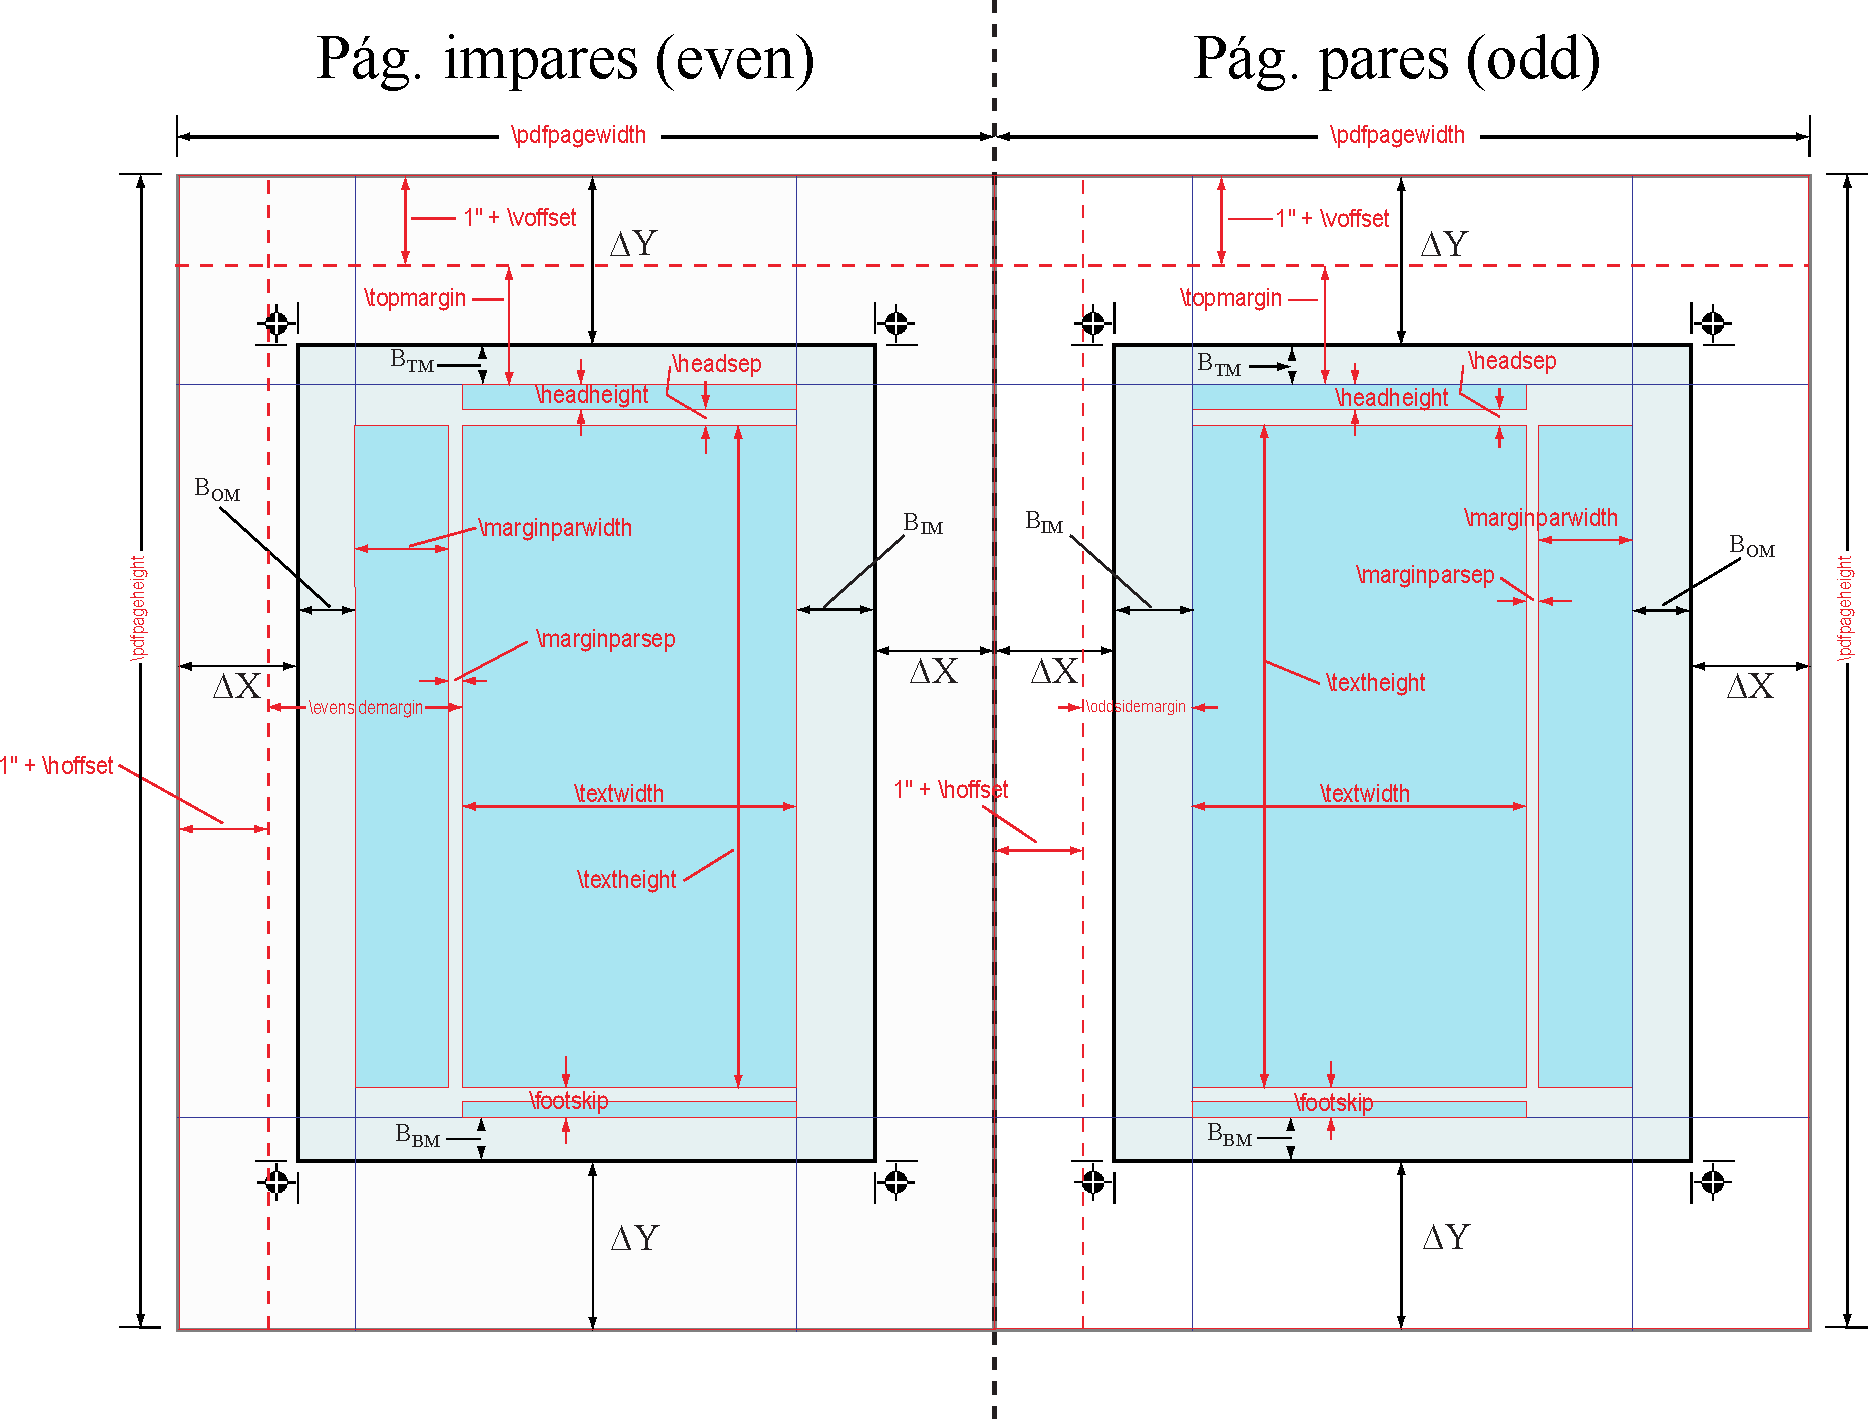
\includegraphics[height=\textheight]{Figuras/layout}
\end{figure}
\end{frame}


\begin{frame}[fragile]{Herramientas para hilar m�s fino}
\begin{itemize}
\item <1-> A veces queremos ajustar alg�n espacio o alguna altura, o forzar cambio de linea
\item <2-> Incluso terminar una p�gina y forzar la creaci�n de otra
\item <3-> Los comandos que m�s se emplean son:
\end{itemize}
\only<4->{
\begin{sintax}{Herramientas de espaciado forzado}
\texttt{\backS vspace\{}{\em valor}\texttt{\}}\\
\texttt{\backS hspace\{}{\em valor}\texttt{\}}\\
\texttt{\backS newpage}\\
\texttt{\backS newline} o bien \texttt{\backS \backS} o bien \texttt{\backS par}
\end{sintax}
}
\pause\pause\pause\pause
\begin{minipage}{0.45\textwidth}
\vspace{-0.2cm}
\begin{ejem}{Espaciado forzado}
\vspace{-0.5cm}
\begin{lstlisting}
Esto \hspace{0.5cm} y esto est�n\newline \vspace{0.4cm} separados por lo que he \\ querido
\end{lstlisting}
\end{ejem}
\end{minipage}%
\pause%
\hfill%
\begin{minipage}{0.45\textwidth}
Esto \hspace{0.5cm} y esto est�n \newline \vspace{0.3cm} separados por lo que he \\ querido
\end{minipage}%
\end{frame}

%----------------------------------------%----------------------------------------%----------------------------------------
\subsection{Referencias cruzadas}
\begin{frame}[fragile]{Referencias}
\only<1->{
\begin{minipage}{0.6\textwidth}
\begin{itemize}
\item <1->Las referencias {\color{miverdeO}complementan} la lectura de un documento, {\color{miverdeO}facilit�ndola}
\item <2-> \LaTeX{} \alert<2>{actualizar�} los marcadores de referencia \alert<2>{autom�ticamente} si se intercalan otras \bien
\item <3-> Los comandos son \texttt{\backS ref} y \texttt{\backS pageref} complementados con \texttt{\backS label} en cualquier parte del documento
\end{itemize}
\end{minipage}}%
\hfill%
\only<4->{
\begin{minipage}{0.39\textwidth}
\begin{sintax}{Referencias}
\texttt{\backS label\{}{\em etiqueta}\texttt{\}}\\
\vdots

\texttt{\backS ref\{}{\em etiqueta}\texttt{\}}\\
y/o\\
\texttt{\backS pageref\{}{\em etiqueta}\texttt{\}}
\end{sintax}
\end{minipage}
}

\pause\pause\pause\pause

\begin{minipage}{0.5\textwidth}
\vspace{-0.2cm}
\begin{ejem}{Referencias}
\vspace{-0.5cm}
\begin{lstlisting}
%etiquetado
\section{Secci�n arbitraria}
{\bf PALABRAS IMPORTANTES}\label{etiqueta}
%. . .
%llamada a la referencia
En la secci�n \ref{etiqueta} de la p�gina \pageref{etiqueta} se dicen unas palabras
\end{lstlisting}
\end{ejem}
\end{minipage}%
\pause%
\hfill%
\begin{minipage}{0.39\textwidth}
\begin{figure}
\centering
\begin{tikzpicture}
\alt<4->{\node[opacity=1]{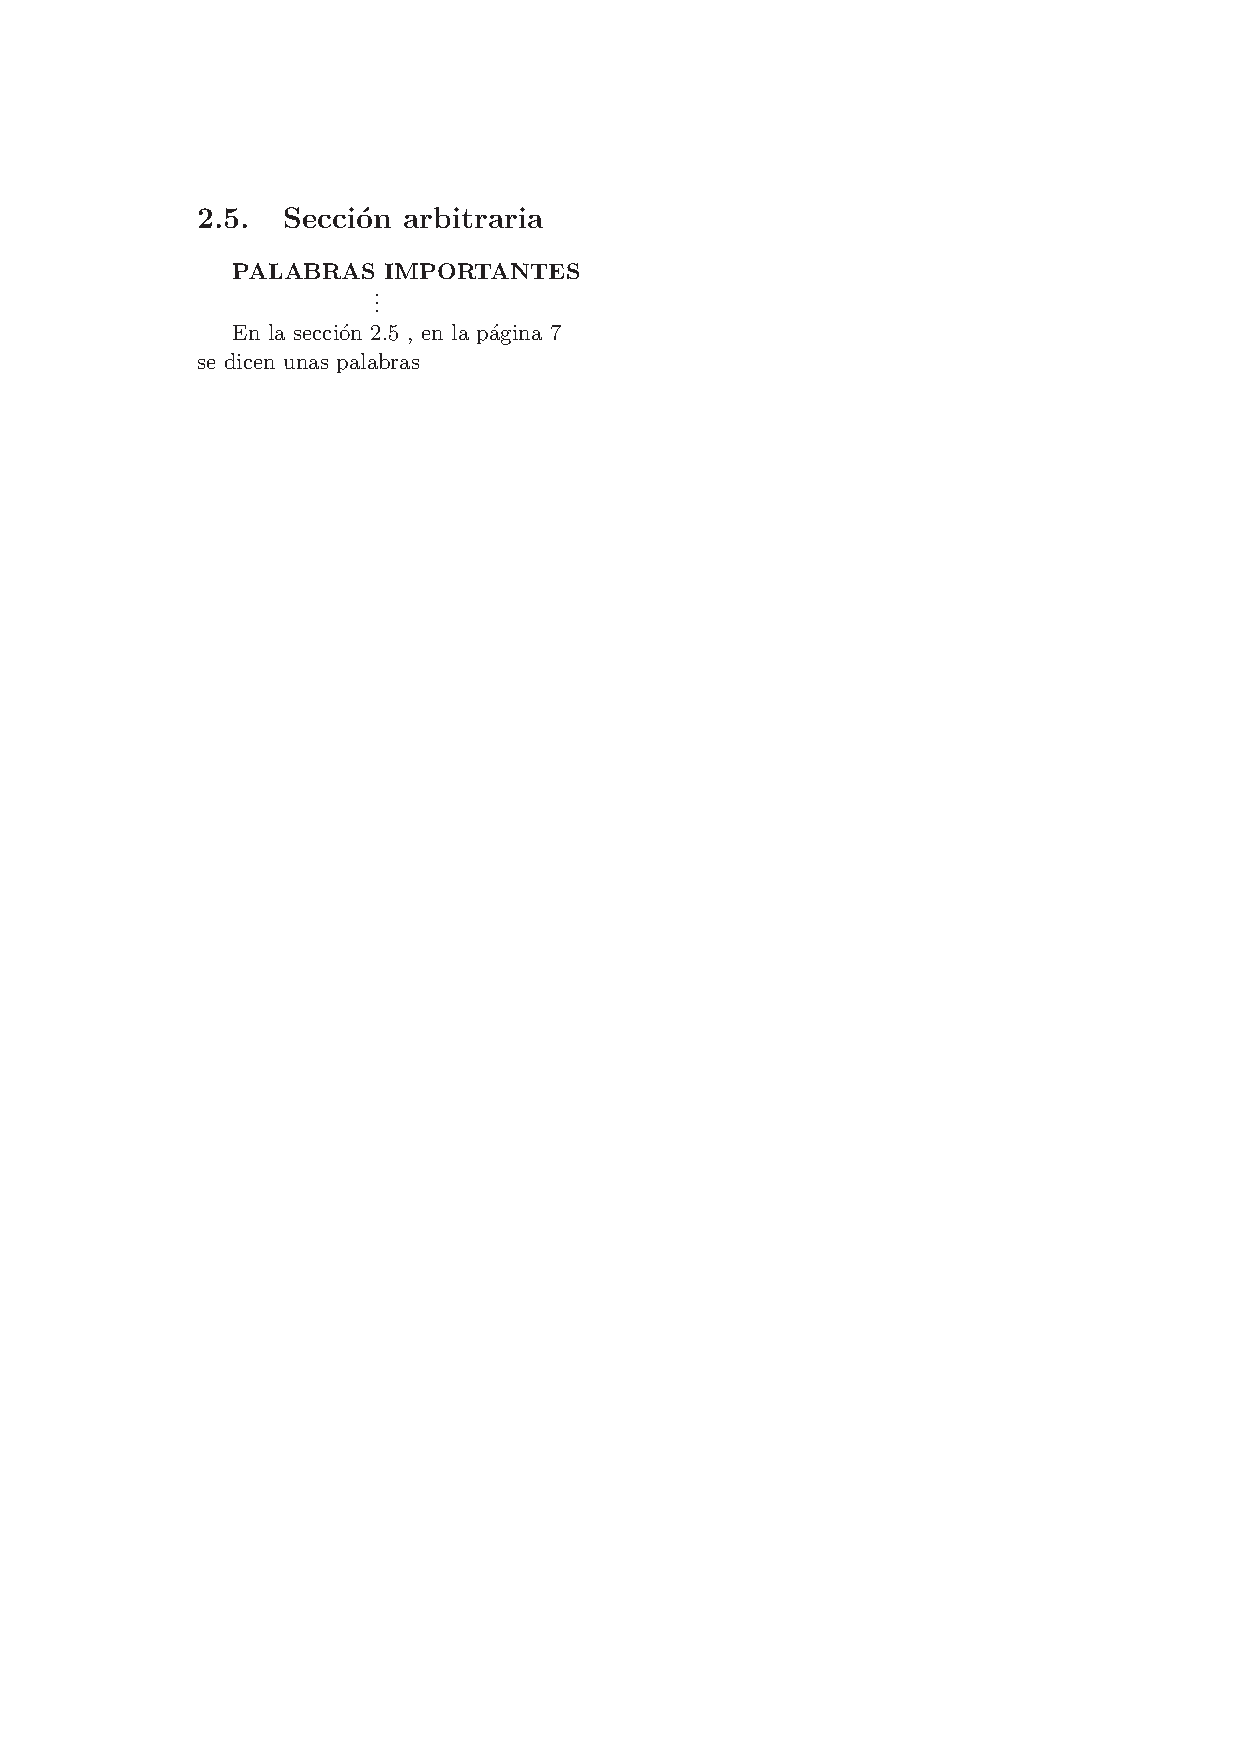
\includegraphics[width=\textwidth]{FigurasEjemplos/referencia}};}
{\node[opacity=0.01]{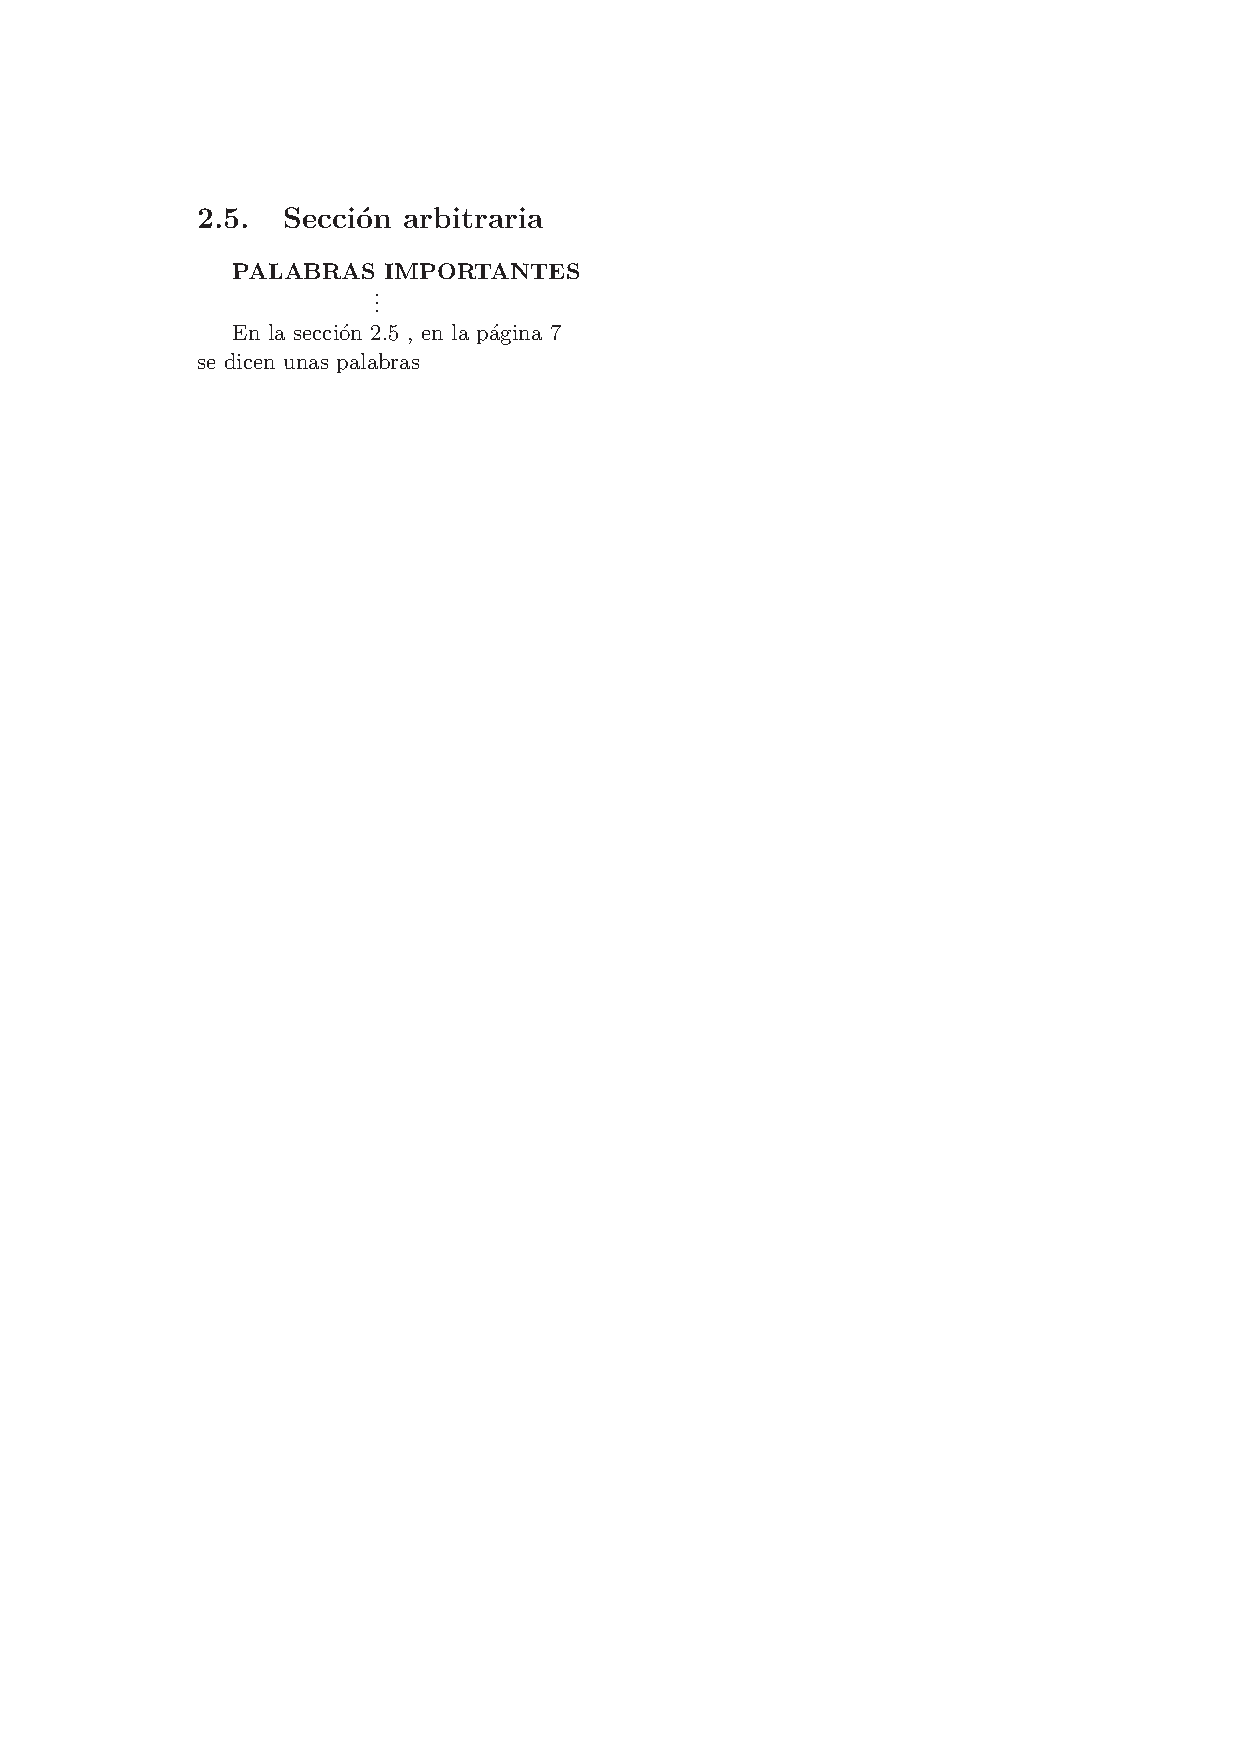
\includegraphics[width=\textwidth]{FigurasEjemplos/referencia}};}
\end{tikzpicture}
\end{figure}
\end{minipage}
\end{frame}
%----------------------------------------%----------------------------------------%----------------------------------------



\subsection{�Manos a la obra!}

\begin{frame}[fragile]{Nuestro ejemplo: Report }
\vspace{-0.1cm}
\begin{center}
\only<1>{
Vamos a a�adir un nuevo cap�tulo con todo lo aprendido en esta lecci�n.}
\only<2->{
\begin{minipage}{0.32\textwidth}
\begin{figure}[hbtp]
\centering
\fbox{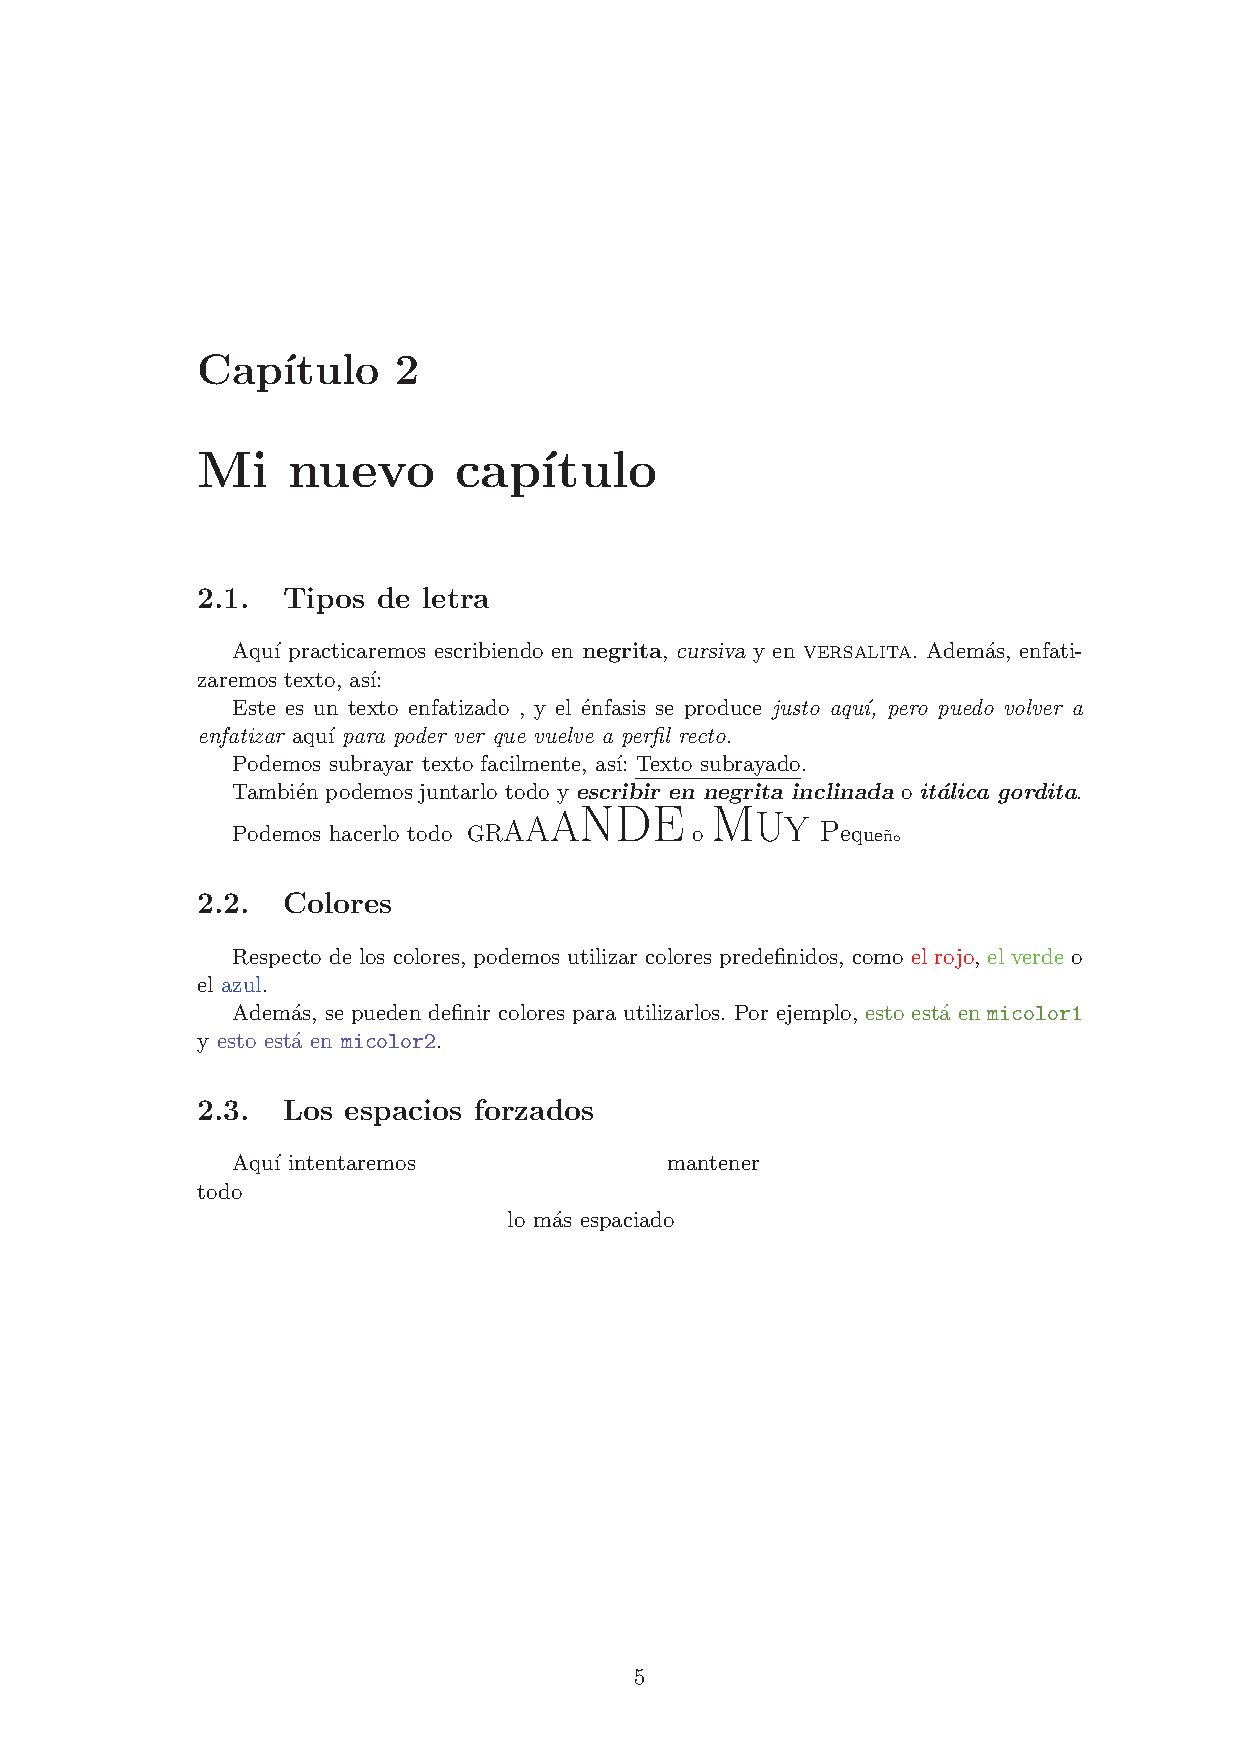
\includegraphics[width=\textwidth, page=1]{FigurasEjemplos/Ejercicio4}}
\end{figure}
\end{minipage}%
\hspace{1cm}
\begin{minipage}{0.32\textwidth}
\begin{figure}[hbtp]
\centering
\fbox{\includegraphics[width=\textwidth, page=2]{FigurasEjemplos/Ejercicio4}}
\end{figure}
\end{minipage}}
\end{center}
\end{frame}

\begin{frame}[fragile]{Nuestro ejemplo: Report}
\vspace{-0.5cm}
\begin{lstlisting}
%-----Pre�mbulo
\usepackage{xcolor}
\definecolor{micolor1}{RGB}{100, 150, 15}
\definecolor{micolor2}{RGB}{100, 50, 255}
\pagestyle{headings}% estilo
\textwidth 15cm
\textheight 24cm
\hoffset -0.2cm
\voffset -1cm
\oddsidemargin 1cm
\evensidemargin 1cm
%-----
\end{lstlisting}
\end{frame}

\begin{frame}[fragile]{Nuestro ejemplo: Report}
\vspace{-0.5cm}
\begin{lstlisting}
%-----Cuerpo
%. . .
\chapter{Mi nuevo cap�tulo}
\section{Tipos de letra}\label{Etiqueta1}
Aqu� practicaremos escribiendo en \textbf{negrita}, {\sl cursiva} y en {\sc versalita}. Adem�s, enfatizaremos texto, as�:

Este es un  texto enfatizado , y el �nfasis se produce {\em justo aqu�, pero puedo volver a enfatizar {\em aqu�} para poder ver que vuelve a perfil recto.}

Podemos subrayar texto facilmente, as�: \underline{Texto subrayado}.

Tambi�n podemos juntarlo todo y \textsl{\bfseries escribir en negrita inclinada} o \textit{\bfseries it�lica gordita}.

Podemos hacerlo todo { G\large R\Large A\LARGE A\huge A\Huge NDE} o {\Huge M\huge U\LARGE Y \Large P\large e\normalsize q\small u\footnotesize e\scriptsize �\tiny o}
\section{Colores}

Respecto de los colores, podemos utilizar colores predefinidos, como {\color{red} el rojo}, {\color{green} el verde} o el {\color{blue} azul}.

Adem�s, se pueden definir colores para utilizarlos. Por ejemplo, {\color{micolor1} esto est� en \texttt{micolor1}} y {\color{micolor2} esto est� en \texttt{micolor2}}.

\section{Los espacios forzados}
Aqu� intentaremos \hspace{4cm} mantener \newline todo\\ \vspace{1cm} \hspace{5cm} lo m�s espaciado\newpage posible
\section{Referencias cruzadas}

En esta secci�n haremos referencia a la secci�n \ref{Etiqueta1} que se encuentra en la p�gina \pageref{Etiqueta1}.
% . . .
\end{lstlisting}

\end{frame}




\section{Las matem�ticas}
\begin{frame}[fragile]{Introducci�n}
\only<1>{En esta lecci�n aprenderemos a declarar el entorno matem�tico y a escribir algunas f�rmulas y ecuaciones}
\only<2-6>{
\begin{minipage}{0.5\textwidth}
\begin{itemize}
\item <2-6> Utilizaremos el paquete \texttt{amsmath}
\item <4-6> Hay dos entornos matem�ticos:
\only<5-6>{
\begin{itemize}
\item Ordinario: En la misma l�nea del texto
\item Resaltado: cambia de l�nea y se centra. Operadores mayores.
\end{itemize}
}
\end{itemize}
\end{minipage}}%
\only<3-6>{
\hfill%
\begin{minipage}{0.4\textwidth}
\begin{paquete}{\texttt{amsmath}}
\texttt{\backS usepackage\{amsmath\}}
\end{paquete}
\end{minipage}}
\only<6->{
\begin{sintax}{Modo matem�tico}
\texttt{\&}{\em f�rmula}\texttt{\&}\dotfill (Modo ordinario)\\
\texttt{\&\&}{\em f�rmula}\texttt{\&\&}\dotfill (Modo resaltado)\\
\texttt{\backS begin\{}{\em equation}\texttt{\}}\\
{\em f�rmula}\\
\texttt{\backS end\{}{\em equation}\texttt{\}}\dotfill (Modo resaltado etiquetado)
\end{sintax}
}
\pause\pause\pause\pause\pause\pause

\begin{minipage}{0.4\textwidth}
\vspace{-0.2cm}
\begin{ejem}{Modo matem�tico}
\vspace{-0.5cm}
\begin{lstlisting}
%ordinario
Sea $f=x^2+1$. La funci�n es continua y derivable en $\mathbb{R}$ con derivada 
%resaltado
$$\frac{df}{dx}=2x$$
%resaltado y enumerado
Y esta es la integral
\begin{equation}
\int{f(x)}=\frac{1}{3}x^3+x
\end{equation}
\end{lstlisting}
\end{ejem}
\end{minipage}%
\pause%
\hfill%
\begin{minipage}{0.55\textwidth}
Sea $f=x^2+1$. La funci�n es continua y derivable en $\mathbb{R}$ con derivada $$\frac{df}{dx}=2x$$
Y esta es la integral
\begin{equation}
\int{f(x)}=\frac{1}{3}x^3+x
\end{equation}
\end{minipage}

\end{frame}

\subsection{Los s�mbolos en matem�ticas}

\begin{frame}[fragile]{Los s�mbolos y el texto}
\only<1->{
\begin{minipage}{0.5\textwidth}
\LaTeX{} ofrece much�sima versatilidad:
\begin{itemize}
\item <2->Ordinarios: $\alpha, \beta, \partial, 1, A, b, $ \ldots
\item <3->Operadores de tama�o variable: $\int, \cap,$ \ldots
\item <4->Operadores de relaci�n: $=, \in, \subset, \ni, \nparallel$ \ldots
\item <5->Operadores binarios: $+, \cup, \Cap$ \ldots
\item <6->Delimitadores: $\{,\},[,], \lVert, \langle$ \ldots
\end{itemize}
\end{minipage}}%
\only<7->{
\begin{minipage}{0.49\textwidth}
\only<7->{En cuanto al texto:}
\begin{itemize}
\item <8-> El texto en el entorno cient�fico no considera los espacios
\item <9-> Para escribir en el entorno cient�fico se usa el comando \texttt{\backS mbox\{}{\em Texto}\texttt{\}}
\end{itemize}
\end{minipage}}


\pause\pause\pause\pause\pause\pause\pause\pause\pause

\begin{minipage}{0.49\textwidth}
\begin{ejem}{Texto en matem�ticas}
\vspace{-0.5cm}
\begin{lstlisting}
$Texto en entorno matem�tico MAL$\\
$\mbox{Texto en entorno matem�tico BIEN}$
\end{lstlisting}
\end{ejem}
\end{minipage}%
\pause%
\hfill%
\begin{minipage}{0.4\textwidth}
$Texto en entorno matem�tico MAL$\\
$\mbox{Texto en entorno matem�tico BIEN}$
\end{minipage}
\end{frame}

\subsection{Sub�ndices, super�ndices y puntos suspensivos}

\begin{frame}[fragile]{Sub�ndices, super�ndices y puntos suspensivos}
\pause
\begin{minipage}{0.24\textwidth}
\begin{itemize}
\item {\bf  Los super�ndices}
\end{itemize}
\end{minipage}%
\pause%
\hfill%
\begin{minipage}{0.27\textwidth}
\begin{sintax}{Super�ndices}
\centering
\texttt{\$}{\em base}\texttt{\^{}\{}{\em exponente}\texttt{\}\$}
\end{sintax}
\end{minipage}%
\pause%
\hfill%
\begin{minipage}{0.24\textwidth}
\begin{ejem}{Super�ndices}
\vspace{-0.5cm}
\begin{lstlisting}
$x^{2x+2}$
\end{lstlisting}
\end{ejem}
\end{minipage}%
\pause%
\hfill%
\begin{minipage}{0.1\textwidth}
$x^{2x+2}$
\end{minipage}

\pause
\begin{minipage}{0.24\textwidth}
\begin{itemize}
\item {\bf  Los sub�ndices} 
\end{itemize}
\end{minipage}%
\pause%
\hfill%
\begin{minipage}{0.26\textwidth}
\begin{sintax}{Sub�ndices}
\centering
\texttt{\$}{\em base}\texttt{\_{}\{}{\em sub�ndice}\texttt{\}\$}
\end{sintax}
\end{minipage}%
\pause%
\hfill%
\begin{minipage}{0.24\textwidth}
\begin{ejem}{Sub�ndices}
\vspace{-0.5cm}
\begin{lstlisting}
$x_{2x+2}$
\end{lstlisting}
\end{ejem}
\end{minipage}%
\pause%
\hfill%
\begin{minipage}{0.1\textwidth}
$x_{2x+2}$
\end{minipage}


\pause
\begin{minipage}{0.18\textwidth}
\begin{itemize}
\item {\bf  Los puntos suspensivos} 
\end{itemize}
\end{minipage}%
\pause%
\hfill%
\begin{minipage}{0.30\textwidth}
\begin{sintax}{Puntos suspensivos}
\centering
\texttt{\$\backS vdots\$}\\
\texttt{\$\backS ldots\$}\\
\texttt{\$\backS cdots\$}\\
\texttt{\$\backS ddots\$}\\
\end{sintax}
\end{minipage}%
\pause%
\hfill%
\begin{minipage}{0.24\textwidth}
\begin{ejem}{Sub�ndices}
\vspace{-0.5cm}
\begin{lstlisting}
$\vdots$\\
$\ldots$\\
$\cdots$\\
$\ddots$\\
\end{lstlisting}
\end{ejem}
\end{minipage}%
\pause%
\hfill%
\begin{minipage}{0.1\textwidth}
$\vdots$\\
$\ldots$\\
$\cdots$\\
$\ddots$\\
\end{minipage}


\end{frame}

\subsection{Fracciones}

\begin{frame}[fragile]{Fracciones}
\begin{itemize}
\item <1-> Se hace uso del comando \texttt{\backS frac}
\item <2-> Para seguir escribiendo en formato no reducido en numerador y denominador se usar� el comando \alert<4>{\texttt{\backS displaystyle\{}{\em m�s f�rmulas}\texttt{\}}\only<4->{\textbf<4->{Su uso es general}}}
\end{itemize}
\only<3->{
\begin{sintax}{Fracciones: \texttt{\backS frac\{\}\{\}}}
\texttt{\backS frac\{}{\em numerador}\texttt{\}\{}{\em denominador}\texttt{\}}
\end{sintax}
}
\pause\pause\pause
\begin{minipage}{0.7\textwidth}
\begin{ejem}{Fracciones}
\vspace{-0.5cm}
\begin{lstlisting}
$$f_1(x)=\frac{|x^2-1|}{(x^2+y^3)^3}$$
$$f_2(x)=\frac{\displaystyle{\frac{\displaystyle{\int{e^{2x}}+y_3^5}}{2x+y}}}
{\frac{\alpha^\beta}{2x+y}}$$
\end{lstlisting}
\end{ejem}
\end{minipage}%
\pause%
\hfill%
\begin{minipage}{0.29\textwidth}
$$f_1(x)=\frac{|x^2-1|}{(x^2+y^3)^3}$$
$$f_2(x)=\frac{\displaystyle{\frac{\displaystyle{\int{e^{2x}}+y_3^5}}{2x+y}}}
{\frac{\alpha^\beta}{2x+y}}$$
\end{minipage}


\end{frame}



\subsection{Ra�ces}

\begin{frame}[fragile]{Ra�ces}
\begin{itemize}
\item <1-> Se hace uso del comando \texttt{\backS sqrt}
\end{itemize}
\only<2->{
\begin{sintax}{Ra�ces: \texttt{\backS sqrt\{\}\{\}}}
\texttt{\backS sqrt[}{\em n}\texttt{]\{}{\em expresi�n}\texttt{\}}
\end{sintax}
}
\pause\pause
\begin{minipage}{0.7\textwidth}
\begin{ejem}{Ra�ces}
\vspace{-0.5cm}
\begin{lstlisting}
$$\sqrt{|x|y^2(a+b^\alpha)}$$
$$\sqrt[\theta]{\displaystyle{\frac{\displaystyle{\int{e^{2x}}+y_3^5}}{2x+y}}}$$
\end{lstlisting}
\end{ejem}
\end{minipage}%
\pause%
\hfill%
\begin{minipage}{0.29\textwidth}
$$\sqrt{|x|y^2(a+b^\alpha)}$$
$$\sqrt[\theta]{\displaystyle{\frac{\displaystyle{\int{e^{2x}}+y_3^5}}{2x+y}}}$$
\end{minipage}

\end{frame}

\subsection{Sumatorios e integrales}


\begin{frame}[fragile]{Sumatorios e integrales}
\only<1->{
\begin{minipage}{0.48\textwidth}
\begin{itemize}
\item <1-> Su aspecto depende del entorno (ordinario o resaltado)
\item <2-> Para que tomen el aspecto resaltado en medio de un texto: \only<3->{\texttt{\backS displaystyle\{\}}}
\end{itemize}
\end{minipage}}%
\only<4->{
\hfill
\begin{minipage}{0.45\textwidth}
\begin{sintax}{Integral}
\texttt{\backS int\_\{}{\em l�m. inferior}\texttt{\}\^{}\{}{\em l�m. superior}\texttt{\}}
\end{sintax}
\begin{sintax}{Sumatorio}
\texttt{\backS sum\_\{}{\em l�m. inferior}\texttt{\}\^{}\{}{\em l�m. superior}\texttt{\}}
\end{sintax}
\end{minipage}
}

\pause\pause\pause\pause
\begin{minipage}{0.35\textwidth}
\vspace{-1cm}
\begin{ejem}{Sumatorios e integrales}
\vspace{-0.5cm}
\begin{lstlisting}
Esta es una suma $\sum _{n=1}^{N}$ en entorno ordinario y esta es en entorno resaltado $$\sum _{n=1}^{N}$$
Esta es una integral $\int _{n=1}^{+ \infty }$ en entorno ordinario y esta es en entorno resaltado $$\int _{n=1}^{+ \infty }$$
\end{lstlisting}
\end{ejem}
\end{minipage}%
\pause%
\hfill%
\begin{minipage}{0.62\textwidth}
\vspace{0.15cm}
Esta es una suma $\sum _{n=1}^{N}$ en entorno ordinario y esta es en entorno resaltado $$\sum _{n=1}^{N}$$
Esta es una integral $\int _{n=1}^{+\infty}$ en entorno ordinario y esta es en entorno resaltado $$\int _{n=1}^{+ \infty }$$
\end{minipage}
\end{frame}

\subsection{Matrices}

\begin{frame}[fragile]{Matrices (general)}
\only<1->{
\begin{minipage}{0.4\textwidth}
\begin{itemize}
\item <1-> Constituyen  un elemento fundamental del lenguaje cient�fico
\item <2-> Entorno \texttt{array}
\end{itemize}
\end{minipage}}%
\only<4->{
\hfill
\begin{minipage}{0.53\textwidth}
\begin{sintax}{\texttt{array}}
\texttt{\backS begin\{array\}[}{\em posici�n}\texttt{]\{}{\em formato columnas}\texttt{\}}\\
$elem_{11}$ \texttt{\&} $elem_{12}$ \texttt{\&} \ldots  \texttt{\&} $elem_{1m}$ \backS\backS\\
$elem_{11}$ \texttt{\&} $elem_{22}$ \texttt{\&} \ldots  \texttt{\&} $elem_{2m}$ \backS\backS\\
\vdots

$elem_{n1}$ \texttt{\&} $elem_{n2}$ \texttt{\&} \ldots  \texttt{\&} $elem_{nm}$ \backS\backS\\
\texttt{\backS end\{array\}}
\end{sintax}
\end{minipage}
}

\pause\pause\pause\pause
\begin{minipage}{0.35\textwidth}
\vspace{-0.5cm}
\begin{ejem}{\texttt{array}}
\vspace{-0.5cm}
\begin{lstlisting}
$$
\begin{array}{cccc}
\|m_1-m_1\|&\|m_1-m_2\|&\cdots  &\|m_1-m_N\|\\
\|m_2-m_1\|&\|m_2-m_2\|&\cdots  &\|m_2-m_N\|\\
\|m_3-m_1\|&\|m_3-m_2\|&\cdots &\|m_3-m_N\|\\
\vdots &\vdots &\ddots &\vdots \\
\|m_N-m_1\|&\|m_N-m_1\|&\cdots &\|m_N-m_N\|\\
\end{array}
$$
\end{lstlisting}
\end{ejem}
\end{minipage}
\pause%
\hfill
\begin{minipage}{0.54\textwidth}
$$
\begin{array}{cccc}
\|m_1-m_1\|&\|m_1-m_2\|&\cdots  &\|m_1-m_N\|\\
\|m_2-m_1\|&\|m_2-m_2\|&\cdots  &\|m_2-m_N\|\\
\|m_3-m_1\|&\|m_3-m_2\|&\cdots &\|m_3-m_N\|\\
\vdots &\vdots &\ddots &\vdots \\
\|m_N-m_1\|&\|m_N-m_1\|&\cdots &\|m_N-m_N\|\\
\end{array}
$$
\end{minipage}
\end{frame}

\begin{frame}[fragile]{Matrices (limitadas)}
\only<1->{
\begin{minipage}{0.59\textwidth}
\begin{itemize}
\item <1-> Simplemente se a�ade el limitador antes y despu�s del entorno \texttt{array}
\item <3-> Limitadores: \texttt{\{, \}, [, ], (, ), |, |}
\end{itemize}
\end{minipage}}%
\only<2->{
\hfill
\begin{minipage}{0.4\textwidth}
\begin{sintax}{\texttt{array} limitado}
\texttt{\backS left} {\em limitador apertura}\\
\texttt{\backS begin\{array\}}\\
\vdots

\texttt{\backS end\{array\}}\\
\texttt{\backS right} {\em limitador cierre}\\
\end{sintax}
\end{minipage}
}

\pause\pause\pause
\begin{minipage}{0.35\textwidth}
\vspace{-0.5cm}
\begin{ejem}{\texttt{array}}
\vspace{-0.5cm}
\begin{lstlisting}
$$
\left[\begin{array}{cccc}
\|m_1-m_1\|&\|m_1-m_2\|&\cdots  &\|m_1-m_N\|\\
\|m_2-m_1\|&\|m_2-m_2\|&\cdots  &\|m_2-m_N\|\\
\|m_3-m_1\|&\|m_3-m_2\|&\cdots &\|m_3-m_N\|\\
\vdots &\vdots &\ddots &\vdots \\
\|m_N-m_1\|&\|m_N-m_1\|&\cdots &\|m_N-m_N\|\\
\end{array}\right]
$$
\end{lstlisting}
\end{ejem}
\end{minipage}
\pause%
\hfill
\begin{minipage}{0.54\textwidth}
\vspace{0.1cm}
$$
\left[\begin{array}{cccc}
\|m_1-m_1\|&\|m_1-m_2\|&\cdots  &\|m_1-m_N\|\\
\|m_2-m_1\|&\|m_2-m_2\|&\cdots  &\|m_2-m_N\|\\
\|m_3-m_1\|&\|m_3-m_2\|&\cdots &\|m_3-m_N\|\\
\vdots &\vdots &\ddots &\vdots \\
\|m_N-m_1\|&\|m_N-m_1\|&\cdots &\|m_N-m_N\|\\
\end{array}\right]
$$
\end{minipage}
\end{frame}

\begin{frame}[fragile]{Matrices (entornos)}
\only<1->{
\begin{minipage}{0.46\textwidth}
\begin{itemize}
\item <1-> Existen entornos que ya incluyen los limitadores
\item <2-> Los entornos son: \texttt{pmatrix}, \texttt{bmatrix}, \texttt{Bmatrix}, \texttt{vmatrix}, \texttt{Vmatrix}
\item <3-> Respectivamente, corresponden a los limitadores \texttt{(), [], \{\}, $|$ $|$} y \texttt{$\|\|$}
\end{itemize}
\end{minipage}}%
\only<4->{
\hfill
\begin{minipage}{0.53\textwidth}
\begin{sintax}{Entornos de matrices}
\texttt{\backS begin\{<?>matrix\}} \\
$elem_{11}$ \texttt{\&} $elem_{12}$ \texttt{\&} \ldots  \texttt{\&} $elem_{1m}$ \backS\backS\\
$elem_{11}$ \texttt{\&} $elem_{22}$ \texttt{\&} \ldots  \texttt{\&} $elem_{2m}$ \backS\backS\\
\vdots

$elem_{n1}$ \texttt{\&} $elem_{n2}$ \texttt{\&} \ldots  \texttt{\&} $elem_{nm}$ \backS\backS\\
\texttt{\backS end\{<?>matrix\}}\\
\end{sintax}
\end{minipage}
}

\pause\pause\pause
\begin{minipage}{0.35\textwidth}
\vspace{-0.3cm}
\begin{ejem}{\texttt{<?>matrix}}
\vspace{-0.5cm}
\begin{lstlisting}
$$
\begin{pmatrix}
\|m_1-m_1\|&\|m_1-m_2\|&\cdots  &\|m_1-m_N\|\\
\|m_2-m_1\|&\|m_2-m_2\|&\cdots  &\|m_2-m_N\|\\
\|m_3-m_1\|&\|m_3-m_2\|&\cdots &\|m_3-m_N\|\\
\vdots &\vdots &\ddots &\vdots \\
\|m_N-m_1\|&\|m_N-m_1\|&\cdots &\|m_N-m_N\|\\
\end{pmatrix}
$$
\end{lstlisting}
\end{ejem}
\end{minipage}
\pause%
\hfill
\begin{minipage}{0.54\textwidth}
\vspace{0.1cm}
$$
\begin{pmatrix}
\|m_1-m_1\|&\|m_1-m_2\|&\cdots  &\|m_1-m_N\|\\
\|m_2-m_1\|&\|m_2-m_2\|&\cdots  &\|m_2-m_N\|\\
\|m_3-m_1\|&\|m_3-m_2\|&\cdots &\|m_3-m_N\|\\
\vdots &\vdots &\ddots &\vdots \\
\|m_N-m_1\|&\|m_N-m_1\|&\cdots &\|m_N-m_N\|\\
\end{pmatrix}
$$
\end{minipage}
\end{frame}


\subsection{Funciones definidas a tramos}

\begin{frame}[fragile]{Funciones a tramos}
\begin{itemize}
\item <1-> El entorno {\tt array} permite definir funciones a tramos
\item <2->\alert<2>{\textbf<2->{Imprescindible escribir \texttt{\backS right.} o \texttt{\backS left.} donde no haya limitador}}
\item <3-> Mejor con un ejemplo:
\end{itemize}

\pause\pause\pause
\begin{minipage}{0.4\textwidth}
\begin{ejem}{Funciones a tramos}
\vspace{-0.5cm}
\begin{lstlisting}
$$f(x)=\left \{     \begin{array}{ll}
\cos(\frac{1}{x})	&	\mbox{si $x \neq 0$} \\
0				&	\mbox{si $x=0$}
\end{array}	\right.
$$
\end{lstlisting}
\end{ejem}
\end{minipage}%
\pause%
\hfill%
\begin{minipage}{0.5\textwidth}
\only<5->{
$$f(x)=\left \{     \begin{array}{ll}
\cos(\frac{1}{x})	&	\mbox{si $x \neq 0$} \\
0				&	\mbox{si $x=0$}
\end{array}	\right.
$$
}
\end{minipage}

\pause
\begin{minipage}{0.4\textwidth}
\begin{ejem}{Funciones a tramos}
\vspace{-0.5cm}
\begin{lstlisting}
$$f(x, y)=\left [     \begin{array}{ll}
\sin(\frac{1}{x})	&	\mbox{si $x \neq 0$} \\
\frac{\partial f}{\partial x}				&	\mbox{si $x=0$}
\end{array}	\right.
$$
\end{lstlisting}
\end{ejem}
\end{minipage}%
\pause%
\hfill%
\begin{minipage}{0.5\textwidth}
\only<5->{
$$f(x, y)=\left [     \begin{array}{ll}
\sin(\frac{1}{x})	&	\mbox{si $x \neq 0$} \\
\displaystyle{\frac{\partial f}{\partial x}}				&	\mbox{si $x=0$}
\end{array}	\right.
$$
}
\end{minipage}


\end{frame}

\subsection{Ecuaciones}

\begin{frame}[fragile]{Ecuaciones}
\begin{itemize}
\item <1-> Las ecuaciones van en el entorno \texttt{equation}, \textbf<2>{sin \texttt{\$} o \texttt{\$\$}}
\item <3-> Se referencian como solemos: con el comando \texttt{\backS label} y \texttt{\backS ref}
\end{itemize}


\pause\pause\pause
\begin{minipage}{0.4\textwidth}
\begin{ejem}{Ecuaciones}
\vspace{-0.5cm}
\begin{lstlisting}

A continuaci�n se muestra la ecuaci�n fundamental a la que nos referiremos de ahora en adelante:

\begin{equation}\label{eq: fundamental}
f(x)=e^{x\cdot\|{x^{15}}\|}
\end{equation}

% . . . 

En la ecuaci�n \ref{eq: fundamental} podemos sustituir el valor absoluto por una ecuaci�n en diferencias \ldots % . . .
\end{lstlisting}
\end{ejem}
\end{minipage}%
\pause%
\hfill%
\begin{minipage}{0.5\textwidth}
\begin{figure}[hbtp]
\centering
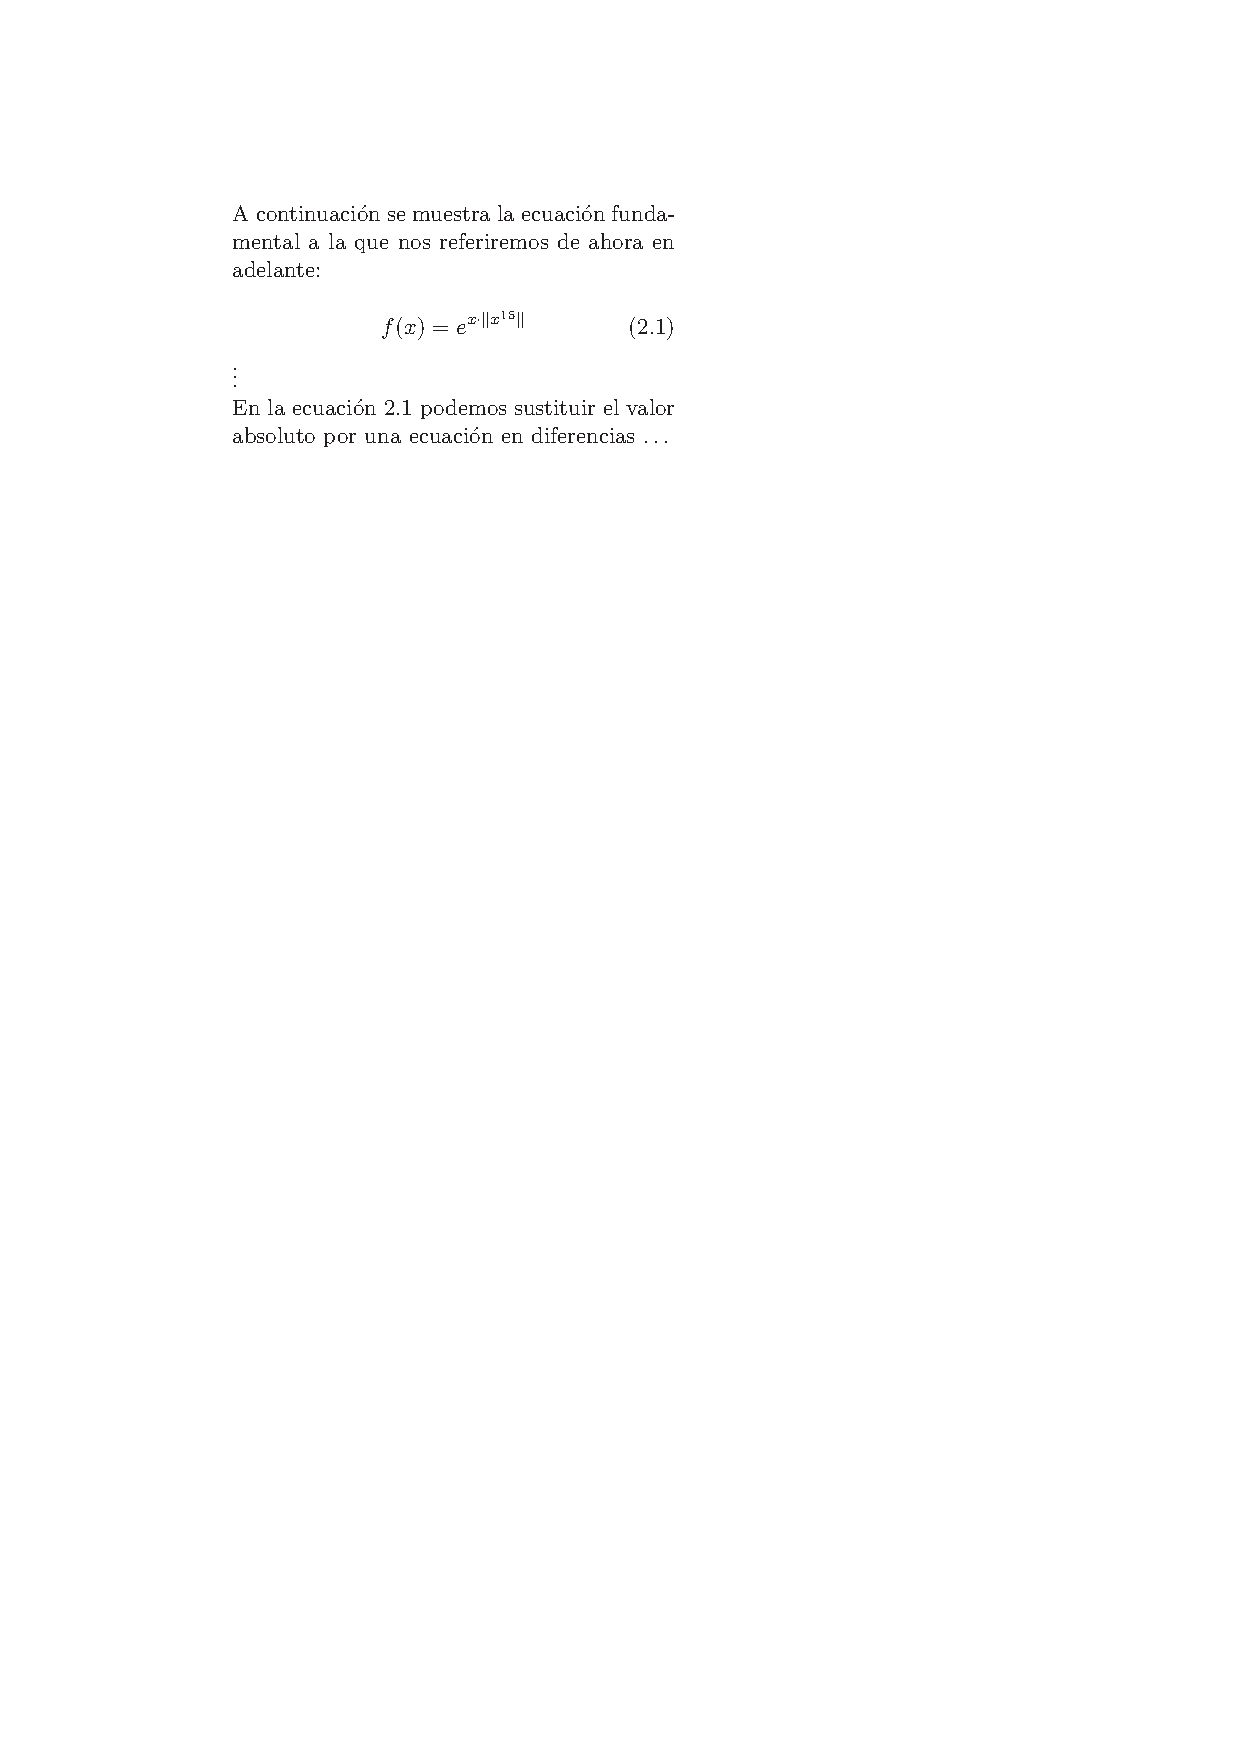
\includegraphics[width=\textwidth, page=1]{FigurasEjemplos/equation}
\end{figure}
\end{minipage}

\end{frame}






%\subsection{S�mbolos cient�ficos}
%
%\begin{frame}[fragile]{Letras griegas}
%Hola
%\end{frame}
%
%\begin{frame}[fragile]{Operadores binarios}
%Hola
%\end{frame}
%
%\begin{frame}[fragile]{Operadores relacionales}
%Hola
%\end{frame}
%
%\begin{frame}[fragile]{Miscel�nea}
%Hola
%\end{frame}
%
%\begin{frame}[fragile]{Fuentes en el entorno matem�tico}
%Hola
%\end{frame}













\subsection{�Manos a la obra!}

\begin{frame}[fragile]{Nuestro ejemplo: Report }
\vspace{-0.1cm}
\begin{center}
\only<1>{
Vamos a a�adir un nuevo cap�tulo con todo lo aprendido en esta lecci�n.}
\only<2->{
\begin{minipage}{0.32\textwidth}
\begin{figure}[hbtp]
\centering
\fbox{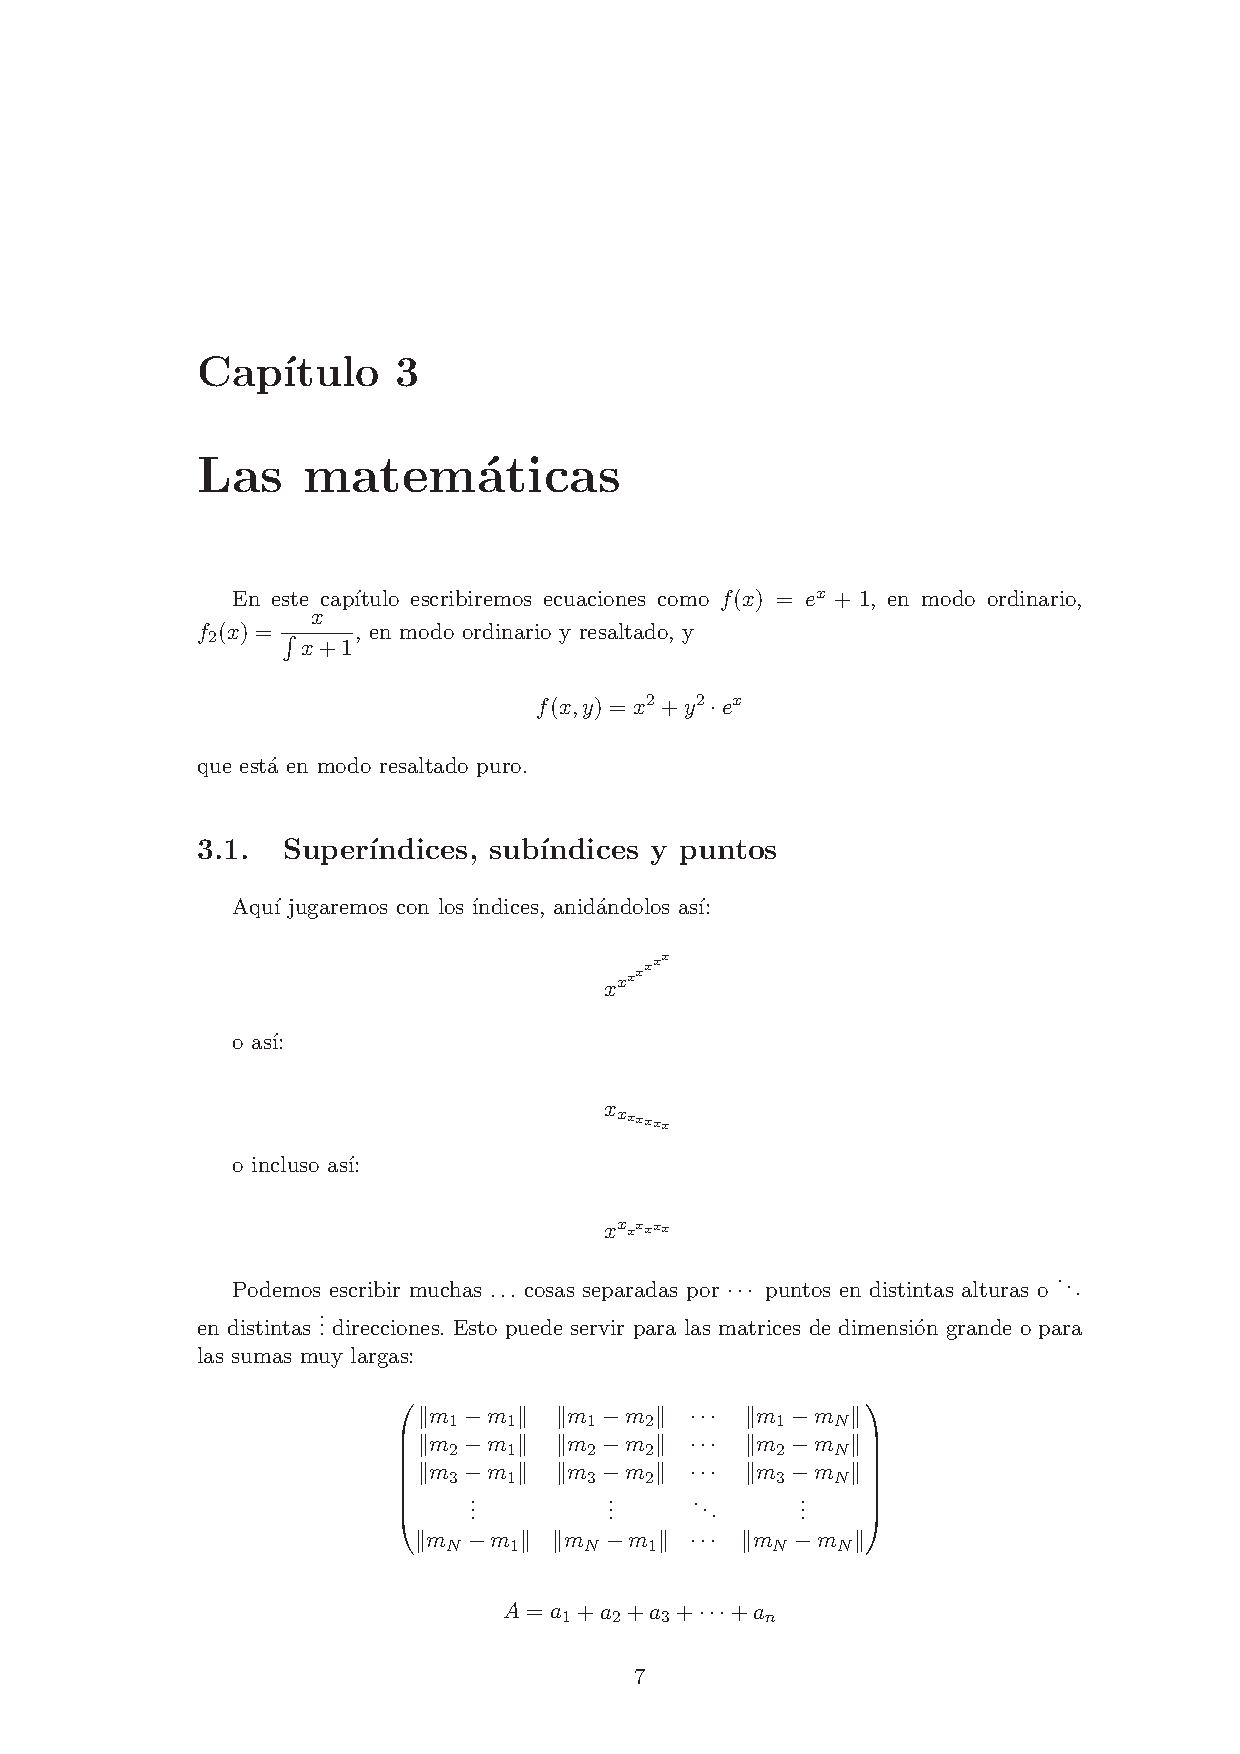
\includegraphics[width=\textwidth, page=1]{FigurasEjemplos/Ejercicio5}}
\end{figure}
\end{minipage}%
\hspace{1cm}
\begin{minipage}{0.32\textwidth}
\begin{figure}[hbtp]
\centering
\fbox{\includegraphics[width=\textwidth, page=2]{FigurasEjemplos/Ejercicio5}}
\end{figure}
\end{minipage}}
\end{center}
\end{frame}



\begin{frame}[fragile]{Nuestro ejemplo: Report }
\vspace{-0.1cm}
\begin{center}
\only<1>{
\begin{minipage}{0.32\textwidth}
\begin{figure}[hbtp]
\centering
\fbox{\includegraphics[width=\textwidth, page=3]{FigurasEjemplos/Ejercicio5}}
\end{figure}
\end{minipage}%
\hspace{1cm}
\begin{minipage}{0.32\textwidth}
\begin{figure}[hbtp]
\centering
\fbox{\includegraphics[width=\textwidth, page=4]{FigurasEjemplos/Ejercicio5}}
\end{figure}
\end{minipage}}
\end{center}
\end{frame}





\begin{frame}[fragile]{Nuestro ejemplo: Report}
\vspace{-0.5cm}
\begin{lstlisting}
\chapter{Las matem�ticas}
En este cap�tulo escribiremos ecuaciones como $f(x)=e^x+1$, en modo ordinario, $\displaystyle{f_2(x)=\frac{x}{\int{x+1}}}$, en modo ordinario y resaltado, y $$f(x, y)=x^2+y^2\cdot e^x$$ que est� en modo resaltado puro.

\section{Super�ndices, sub�ndices y puntos}
Aqu� jugaremos con los �ndices, anid�ndolos as�:
$$x^{x^{x^{x^{x^{x^{x}}}}}}$$
o as�:
$$x_{x_{x_{x_{x_{x_{x}}}}}}$$
o incluso as�:
$$x^{x_{x^{x_{x^{x_{x}}}}}}$$
Podemos escribir muchas $\ldots$ cosas separadas por $\cdots$ puntos en distintas alturas o $\ddots$ en distintas $\vdots$ direcciones.
 Esto puede servir para las matrices de dimensi�n grande o para las sumas muy largas:
$$
\begin{pmatrix}
\|m_1-m_1\|&\|m_1-m_2\|&\cdots  &\|m_1-m_N\|\\
\|m_2-m_1\|&\|m_2-m_2\|&\cdots  &\|m_2-m_N\|\\
\|m_3-m_1\|&\|m_3-m_2\|&\cdots &\|m_3-m_N\|\\
\vdots &\vdots &\ddots &\vdots \\
\|m_N-m_1\|&\|m_N-m_1\|&\cdots &\|m_N-m_N\|\\
\end{pmatrix}
$$

$$A=a_1+a_2+a_3+\cdots+a_n$$
\end{lstlisting}
\end{frame}







\begin{frame}[fragile]{Nuestro ejemplo: Report}
\vspace{-0.5cm}
\begin{lstlisting}
\section{Fracciones}
Respecto de las fracciones denemos que decir que se pueden anidar, por supuesto:
$$\frac{\frac{a}{b}}{\frac{a+c}{b+x^2}}$$

Pero queda mejor con \texttt{\textbackslash displaystyle}:
$$\displaystyle{\frac{\displaystyle{\frac{a}{b}}}{\displaystyle{\frac{a+c}{b+x^2}}}}$$

Evidentemente, se puede unir todo lo anterior:
$$
F=
\displaystyle{\frac{\displaystyle{\frac{x^{x^{x^{x^{x^{x^{x}}}}}}}{x_{x_{x_{x_{x_{x_{x}}}}}}}}}{\displaystyle{\frac{
\begin{pmatrix}
\|m_1-m_1\|&\|m_1-m_2\|&\cdots  &\|m_1-m_N\|\\
\|m_2-m_1\|&\|m_2-m_2\|&\cdots  &\|m_2-m_N\|\\
\|m_3-m_1\|&\|m_3-m_2\|&\cdots &\|m_3-m_N\|\\
\vdots &\vdots &\ddots &\vdots \\
\|m_N-m_1\|&\|m_N-m_1\|&\cdots &\|m_N-m_N\|\\
\end{pmatrix}
}{
A=a_1+a_2+a_3+\cdots+a_n
}}}}
$$
\end{lstlisting}
\end{frame}


\begin{frame}[fragile]{Nuestro ejemplo: Report}
\vspace{-0.5cm}
\begin{lstlisting}
\section{Ra�ces}
Las ra�ces se tragan cualquier cosa, es decir, podemos escribir dentro de ellas todo lo que queramos, solo hay que prestar atenci�n a los limitadores de los entornos:
$$
G=
\sqrt[a_1+a_2+a_3+\cdots+a_n]{
\begin{pmatrix}
\|m_1-m_1\|&\|m_1-m_2\|&\cdots  &\|m_1-m_N\|\\
\|m_2-m_1\|&\|m_2-m_2\|&\cdots  &\|m_2-m_N\|\\
\|m_3-m_1\|&\|m_3-m_2\|&\cdots &\|m_3-m_N\|\\
\vdots &\vdots &\ddots &\vdots \\
\|m_N-m_1\|&\|m_N-m_1\|&\cdots &\|m_N-m_N\|\\
\end{pmatrix}
}
=
\sqrt[A]{
\displaystyle{\frac{x^{x^{x^{x^{x^{x^{x}}}}}}}{x_{x_{x_{x_{x_{x_{x}}}}}}}}
}
$$

\section{Sumatorios e integrales}
Aqu� escribiremos integrales en el texto as�: $\int_{-1}^{+\infty}x^3$, tambi�n as�:  $\displaystyle{\int_{-1}^{+\infty}x^3}$ e incluso as�: $$\int_{-1}^{+\infty}x^3$$

Lo mismo haremos con la suma: $\sum_{-1}^{+\infty}x^3$, tambi�n as�:  $\displaystyle{\sum_{-1}^{+\infty}x^3}$ e incluso as�: $$\sum_{-1}^{+\infty}x^3$$
\end{lstlisting}
\end{frame}



\begin{frame}[fragile]{Nuestro ejemplo: Report}
\vspace{-0.5cm}
\begin{lstlisting}
\section{Matrices}

Aqu� simplemente aplicaremos algunos ejemplos para los limitadores. N�tese que en cada elemento puede entrar cualquier cosa.

$$
\begin{pmatrix}
\begin{Vmatrix}
\|m_1-m_1\|&\|m_1-m_2\|&\cdots  &\|m_1-m_N\|\\
\|m_2-m_1\|&\|m_2-m_2\|&\cdots  &\|m_2-m_N\|\\
\|m_3-m_1\|&\|m_3-m_2\|&\cdots &\|m_3-m_N\|\\
\vdots &\vdots &\ddots &\vdots \\
\|m_N-m_1\|&\|m_N-m_1\|&\cdots &\|m_N-m_N\|\\
\end{Vmatrix}                                                                &\|m_1-m_2\|&\cdots  &\|m_1-m_N\|\\
a_1+a_2+a_3+\cdots+a_n&\displaystyle{\sum_{-1}^{+\infty}x^3}&\cdots  &\displaystyle{\frac{x^{x^{x^{x^{x^{x^{x}}}}}}}{x_{x_{x_{x_{x_{x_{x}}}}}}}}\\
\|m_3-m_1\|&\|m_3-m_2\|&\cdots &\|m_3-m_N\|\\
\vdots &\vdots &\ddots &\vdots \\
\displaystyle{\int_{-1}^{+\infty}x^3}&\|m_N-m_1\|&\cdots &\displaystyle{\sum_{-1}^{+\infty}x^3}\\
\end{pmatrix}
$$

% . . .
\end{lstlisting}
\end{frame}


\begin{frame}[fragile]{Nuestro ejemplo: Report}
\vspace{-0.5cm}
\begin{lstlisting}
\section{Funciones definidas a tramos}
Realizaremos el ejemplo de las diapositivas en primer lugar, y a continuaci�n aplicaremos el anidammiento con algunas de las cosas que hemos escrito hasta ahora:
$$f(x)=\left \{     \begin{array}{ll}
\cos(\frac{1}{x})	&	\mbox{si $x \neq 0$} \\
0				&	\mbox{si $x=0$}
\end{array}	\right.
$$
Si ponemos una matriz y centramos la definici�n del tramo, por ejemplo:

% . . .

Tambi�n podemos hacer lo siguiente:
$$f(x)=\left \{     \begin{array}{ll}
\cos(\frac{1}{x})	&	\mbox{si $x \leq 0$} \\
0				&	\mbox{si $x\in (0, 5]$}\\
\displaystyle{\sum_{-1}^{+\infty}x^3}	&	\mbox{si $x\in (5, 1500]$} \\
0	&	\mbox{si $x\in (1500, 5000]$} \\
\displaystyle{\int_{-1}^{+\infty}x^3}	&	\mbox{si $x\in (6000, +\infty]$} 
\end{array}	\right.
$$
\end{lstlisting}
\end{frame}




\begin{frame}[fragile]{Nuestro ejemplo: Report}
\vspace{-0.5cm}
\begin{lstlisting}
\section{Ecuaciones}
Finalmente podemos poner etiquetas a las ecuaciones anteriores simplemente cambiando la definici�n del entorno, y referenciarlas mediante  \texttt{\textbackslash label} y \texttt{\textbackslash ref}. Por ejemplo:
\begin{equation}\label{eq: ecuacion1}
f(x)=\left \{     \begin{array}{ll}
\cos(\frac{1}{x})	&	\mbox{si $x \neq 0$} \\
0				&	\mbox{si $x=0$}
\end{array}	\right.
\end{equation}
\begin{equation}\label{eq: ecuacion2}
f(x)=\sum_{-1}^{+\infty}x^3
\end{equation}
\begin{equation}\label{eq: ecuacion3}
F=\begin{pmatrix}
\|m_1-m_1\|&\|m_1-m_2\|&\cdots  &\|m_1-m_N\|\\
\|m_2-m_1\|&\|m_2-m_2\|&\cdots  &\|m_2-m_N\|\\
\|m_3-m_1\|&\|m_3-m_2\|&\cdots &\|m_3-m_N\|\\
\vdots &\vdots &\ddots &\vdots \\
\|m_N-m_1\|&\|m_N-m_1\|&\cdots &\|m_N-m_N\|\\
\end{pmatrix}
\end{equation}
\begin{equation}\label{eq: ecuacion4}
f(x)=\left \{     \begin{array}{ll}
\sin\left(\displaystyle{\frac{1}{x}}\right)	&	\mbox{si $x \neq 0$} \\
0				&	\mbox{si $x=0$}
\end{array}	\right.
\end{equation}
Y a continuaci�n referenciarlas: La ecuaci�n \ref{eq: ecuacion2} tiene una suma, la ecuaci�n \ref{eq: ecuacion3} tiene una matriz, la ecuaci�n \ref{eq: ecuacion1} tiene un coseno y la ecuaci�n \ref{eq: ecuacion4} tiene un seno.
\end{lstlisting}
\end{frame}





\section{Los objetos flotantes}

\begin{frame}{Introducci�n}
\only<1-5>{
\begin{itemize}
\item <1-5> Objeto flotante: elemento \alert{desligado} normalmente de la secuencia del texto, que puede ser \alert{referenciado}
\item <2-5> Puede tener tama�o \alert{grande}
\item <3->{ Dos tipos:}
	\only <4-5>{
	\begin{itemize}
	\item Cuadros (contienen tablas)
	\item Figuras (contienen gr�ficos)
	\end{itemize}}
\item <5> {Normalmente habr� varios, e interesa crear un \alert{�ndice} de cada uno de los dos tipos mediante:
	\begin{itemize}
	\item \texttt{\backS listoffigures}
	\item \texttt{\backS listoftables}
	\end{itemize}
}
\end{itemize}
}

\only<6->{
\begin{minipage}{0.6\textwidth}
\only<6->{
\begin{itemize}
\item <6-> La sintaxis general de un objeto flotante es:
\end{itemize}
}

\only<7->{

\begin{sintax}{Objeto flotante}
\texttt{\backS begin\{<figure>|<table>}\texttt{\}[}{\em posici�n}\texttt{]}\\
{\em Objeto}\\
\texttt{\backS caption[}{\em texto en el �ndice}\texttt{]\{}{\em texto en la leyenda}\texttt{\}}\\
\texttt{\backS label\{}{\em etiqueta}\texttt{\}}\only<9->{\dotfill(recomendado)}\\
\texttt{\backS end\{<figure>|<table>\}}
\end{sintax}
}

\only<8->{Donde:
\begin{itemize}
\item <9->\texttt{caption}: Pie de tabla/figura
\item <10->\texttt{label}: Etiqueta para referenciar el objeto
\end{itemize}
}
\end{minipage}%
\only<11->{
\hfill
\begin{minipage}{0.35\textwidth}
Y donde {\em posici�n} puede tomar los valores:
\only<12->{
\begin{itemize}
\item \texttt{h} (here): justo donde est� el entorno
\item \texttt{b} (bottom): abajo de la hoja
\item \texttt{t} (top): arriba de la hoja
\item \texttt{p} (page): en una hoja aparte
\end{itemize}
}
\end{minipage}
}
}


\end{frame}

\subsection{Los cuadros}

\begin{frame}[fragile]{Los cuadros: entorno \texttt{table}}

\begin{minipage}{0.45\textwidth}
\begin{ejem}{Cuadros}
\vspace{-0.5cm}
\begin{lstlisting}
En la siguiente tabla (tabla \ref{tab: NotasClase}) se pueden ver las notas de clase:
\begin{table}[hbtp]
\begin{tabular}{||c|c|c||}
\hline
{\bf Nombre} & {\bf Apellido} & {\bf Puntuaci�n} \\
\hline \hline
Marta & Casc�n & 3.5 \\
Juan & Gonzalez & 6.5 \\
Pedro & Delgado & 9.3 \\
Carlos & Perales & 8 \\
\hline
\end{tabular}
\caption{Notas de clase}
\label{tab: NotasClase}
\end{table}
Y son, en general, bastante satisfactorias.
\end{lstlisting}
\end{ejem}
\end{minipage}%
\pause%
\hfill%
\begin{minipage}{0.49\textwidth}
En el siguiente cuadro (cuadro \ref{tab: NotasClase}) se pueden ver las notas de clase:
\begin{table}[hbtp]
\begin{tabular}{||c|c|c||}
\hline
{\bf Nombre} & {\bf Apellido} & {\bf Puntuaci�n} \\
\hline \hline
Marta & Casc�n & 3.5 \\
Juan & Gonzalez & 6.5 \\
Pedro & Delgado & 9.3 \\
Carlos & Perales & 8 \\
\hline
\end{tabular}
\caption{Notas de clase}
\label{tab: NotasClase}
\end{table}
Y son, en general, bastante satisfactorias.
\end{minipage}

\end{frame}

\subsection{Las figuras}

\begin{frame}[fragile]{Inclusi�n de gr�ficos}
\only<1>{Los gr�ficos en \LaTeX{} pueden ser internos (generados por el editor) o externos (nos centraremos en �stos)}
\only<2-8>{
\begin{minipage}{0.49\textwidth}
Inclusi�n de gr�ficos externos:
\begin{itemize}
\item <2-8> Se emplear� el paquete \texttt{graphicx}
\item <4-8> En sus opciones se carga el compilador (PDF\LaTeX{})
\item <5-8> Formatos aceptados: \textsc{jpg, jpeg, tif, tiff, png} y {\sc pdf}
\item <6-8> Para cargar archivos vectoriales ({\sc eps}) emplearemos el paquete \texttt{epstopdf} para convertirlos a {\sc pdf}
\end{itemize}
\end{minipage}}%
\only<2-8>{
\hfill
\begin{minipage}{0.49\textwidth}
	\only<3-8>{
		\begin{paquete}{\texttt{graphicx}}
		\texttt{\backS usepackage[}{\em opciones}\texttt{]\{graphicx\}} 
		\end{paquete}
	}
	\only<7-8>{
		\begin{paquete}{\texttt{graphicx}}
		\texttt{\backS usepackage\{epstopdf\}} 
		\end{paquete}
	}
\end{minipage}
}
\only<8->{
\begin{sintax}{\texttt{\backS includegraphics}}
\texttt{\backS includegraphics[}{\em opciones}\texttt{]\{}{\em ruta de la figura}\texttt{\}}
\end{sintax}
}
\only<9->{
Las opciones de \texttt{\backS includegraphics} son:
\begin{itemize}
\item \texttt{width$=$}{\em anchura}: Anchura del gr�fico
\item \texttt{height$=$}{\em altura}: Altura del gr�fico
\item \texttt{keepaspectratio$=$}{\em true|false}: Escalado que no puede sobrepasar la mayor restricci�n entre anchura y altura
\item \texttt{scale$=$}{\em escala}: Factor de escala sin considerar restricciones dimensionales
\item \texttt{clip$=$}{\em true|false}: Para recortar la imagen a las dimensiones especificadas
\item \texttt{draft$=$}{\em true|false}: Acelera la compilaci�n: Si {\em true} se deja el hueco pero no se incluye el gr�fico. Si {\em false} se incluye el gr�fico
\end{itemize}
}
\end{frame}






\begin{frame}[fragile]{Las figuras: entorno \texttt{figure}}
\begin{minipage}{0.45\textwidth}
\begin{ejem}{Figuras}
\vspace{-0.5cm}
\begin{lstlisting}
En la figura \ref{fig: Manzana} se puede ver una apetitosa manzana
\begin{figure}[hbtp]
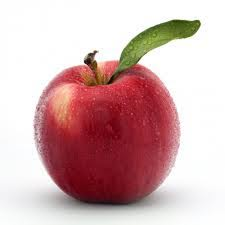
\includegraphics[width=1.5cm]{Figuras/Manzana.jpg}
\caption{La apetitosa manzana}
\label{fig: Manzana}
\end{figure}
El problema es que no puedo ajustar el texto al lado de la figura 
\end{lstlisting}
\end{ejem}
\end{minipage}%
\pause%
\hfill%
\begin{minipage}{0.49\textwidth}
En la figura \ref{fig: Manzana} se puede ver una apetitosa manzana
\begin{figure}[hbtp]
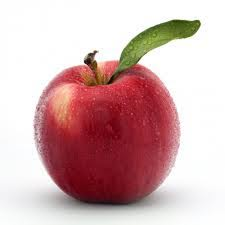
\includegraphics[width=2.5cm]{Figuras/Manzana.jpg}
\caption{La apetitosa manzana}
\label{fig: Manzana}
\end{figure}
El problema es que no puedo ajustar el texto al lado de la figura 

\visible<3->{\centering\mal}
\end{minipage}
\end{frame}



\begin{frame}{Las figuras: entorno \texttt{wrapfigure}}


\only<1>{Este entorno permite ajustar el texto alrededor de un gr�fico}
\only<2->{
\begin{minipage}{0.45\textwidth}
\begin{itemize}
\item <2-> Se emplear� el paquete \texttt{wrapfig}
\item <4-> La sintaxis para su inclusi�n es la siguiente:
\end{itemize}
\end{minipage}}%
\only<2->{
\hfill
\begin{minipage}{0.45\textwidth}
	\only<3->{
		\begin{paquete}{\texttt{wrapfig}}
		\texttt{\backS usepackage\{wrapfig\}} 
		\end{paquete}
	}
\end{minipage}
}
\only<5->{
\begin{sintax}{\texttt{\backS wrapfigure}}
\texttt{\backS begin\{wrapfigure\}\{}{\em alineaci�n del gr�fico}\texttt{\}\{}{\em anchura del gr�fico}\texttt{\}}\\
{\em Objeto}\\
\texttt{\backS caption[}{\em texto en el �ndice}\texttt{]\{}{\em texto en la leyenda}\texttt{\}}\\
\texttt{\backS label\{}{\em etiqueta}\texttt{\}}\\
\texttt{\backS end\{wrapfigure\}}
\end{sintax}
}
\end{frame}





\begin{frame}[fragile]{Las figuras: entorno \texttt{wrapfigure}}


\begin{minipage}{0.45\textwidth}
\begin{ejem}{Figuras}
\vspace{-0.5cm}
\begin{lstlisting}
En la figura \ref{fig: Manzana} se puede ver una apetitosa manzana
\begin{wrapfigure}{r}{0.5\textwidth}
\vspace{-10pt}
\begin{center}
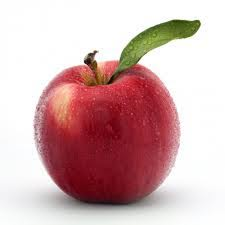
\includegraphics[width=2.5cm, keepaspectratio]{Figuras/Manzana.jpg}
\caption{La apetitosa manzana}
\label{fig: Manzana}
\vspace{-20pt}
\end{center}
\end{wrapfigure}
Pero lo mejor de todo es que sin preocuparme por el formato, \LaTeX{} se encarga de escribir todo lo que ponga a continuaci�n del entorno alrededor de la figura, y si ya ha alcanzado el final, vuelve a el ancho de p�gina original. Por ejemplo, ahora estoy escribiendo de m�s para ver como se vuelve a justificar, y se puede ver perfectamente.
\end{lstlisting}
\end{ejem}
\end{minipage}%
\pause%
\hfill%
\begin{minipage}{0.49\textwidth}
En la figura \ref{fig: Manzana} se puede ver una apetitosa manzana
\begin{wrapfigure}{r}{0.5\textwidth}
\vspace{-10pt}
\begin{center}
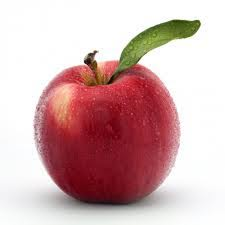
\includegraphics[width=2.5cm, keepaspectratio]{Figuras/Manzana.jpg}
\caption{La apetitosa manzana}
\label{fig: Manzana}
\vspace{-20pt}
\end{center}
\end{wrapfigure}
Pero lo mejor de todo es que sin preocuparme por el formato, \LaTeX{} se encarga de escribir todo lo que ponga a continuaci�n del entorno alrededor de la figura, y si ya ha alcanzado el final, vuelve a el ancho de p�gina original. Por ejemplo, ahora estoy escribiendo de m�s para ver como se vuelve a justificar, y se puede ver perfectamente.
\end{minipage}

\end{frame}










\subsection{�Manos a la obra!}

\begin{frame}[fragile]{Nuestro ejemplo: Report }
\only<1>{
A�adiremos ahora a nuestra memoria los �ndices de figuras y de tablas, as� como un nuevo cap�tulo para los objetos flotantes.
}
\only<2->{
\vspace{-0.1cm}
\begin{center}
\only<2->{
\begin{minipage}{0.32\textwidth}
\begin{figure}[hbtp]
\centering
\fbox{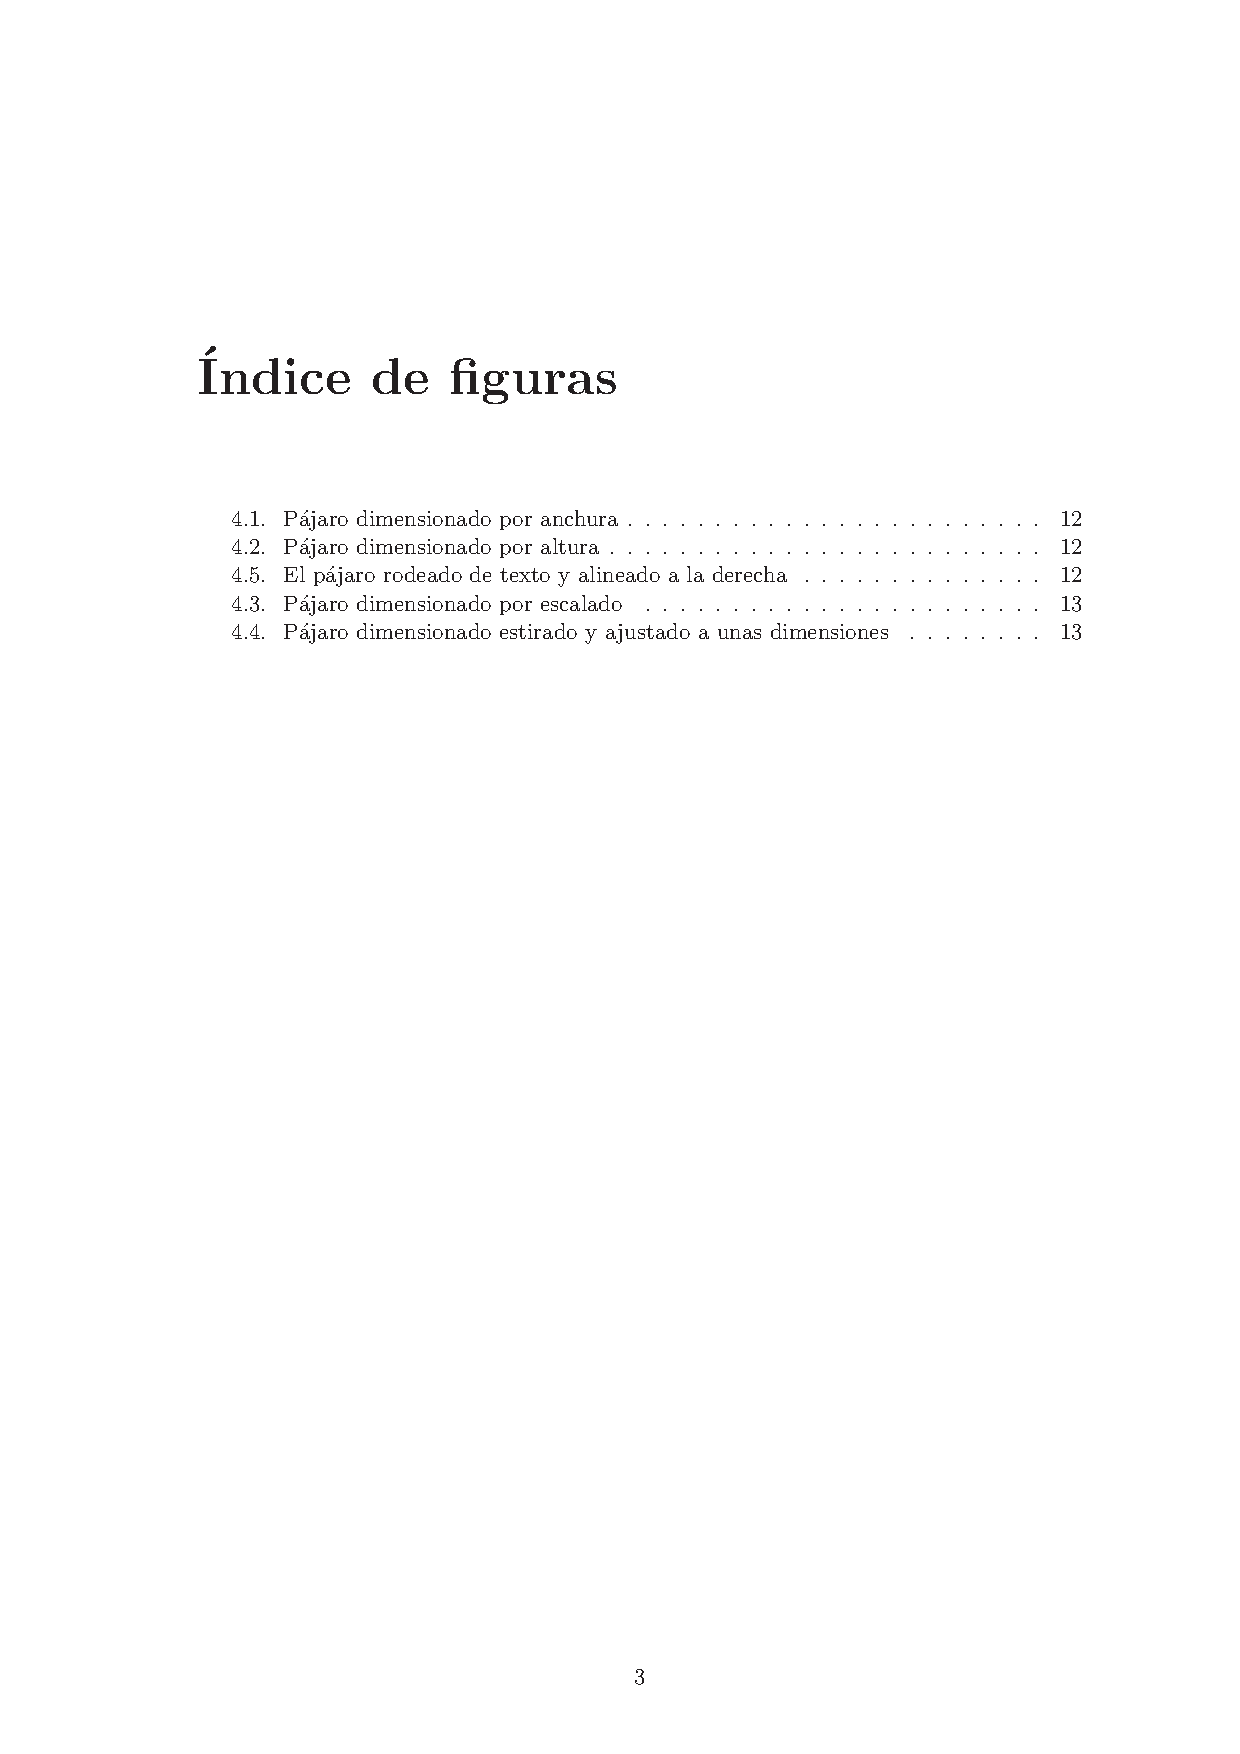
\includegraphics[width=\textwidth, page=1]{FigurasEjemplos/Ejercicio6}}
\end{figure}
\end{minipage}%
\hspace{1cm}}
\only<3->{
\begin{minipage}{0.32\textwidth}
\begin{figure}[hbtp]
\centering
\fbox{\includegraphics[width=\textwidth, page=2]{FigurasEjemplos/Ejercicio6}}
\end{figure}
\end{minipage}}
\end{center}
}
\end{frame}

\begin{frame}[fragile]{Nuestro ejemplo: Report }
\vspace{-0.1cm}
\begin{center}
\only<1->{
\hfill
\begin{minipage}{0.32\textwidth}
\begin{figure}[hbtp]
\centering
\fbox{\includegraphics[width=\textwidth, page=3]{FigurasEjemplos/Ejercicio6}}
\end{figure}
\end{minipage}%
\hfill}
\only<2->{
\begin{minipage}{0.32\textwidth}
\begin{figure}[hbtp]
\centering
\fbox{\includegraphics[width=\textwidth, page=4]{FigurasEjemplos/Ejercicio6}}
\end{figure}
\end{minipage}%
\hfill}
\only<3->{
\begin{minipage}{0.32\textwidth}
\begin{figure}[hbtp]
\centering
\fbox{\includegraphics[width=\textwidth, page=5]{FigurasEjemplos/Ejercicio6}}
\end{figure}
\end{minipage}}
\end{center}
\end{frame}





\begin{frame}[fragile]{Nuestro ejemplo: Report}
\vspace{-0.75cm}
\begin{lstlisting}
\chapter{Los objetos flotantes}
Aqu� aplicaremos los dos entornos m�s usados relacionados con los objetos flotantes: las figuras y las tablas.
\section{Las tablas o cuadros}
Las tablas pueden ser un entorno simplemente que se incluye en el texto:
\begin{center}
\begin{tabular}{||c|c|c||}
\hline
{\bf Nombre} & {\bf Apellido} & {\bf Puntuaci�n} \\
\hline \hline
Marta & Casc�n & 3.5 \\
Juan & Gonzalez & 6.5 \\
Pedro & Delgado & 9.3 \\
Carlos & Perales & 8 \\     \hline
\end{tabular}
\end{center}
O se puede tratar de un entorno que se pueda referenciar como tabla, aparecer ordenado en un �ndice de tablas, poder ser editado en cuanto a posici�n y apariencia, etc.
\begin{table}[h]
\begin{center}
\begin{tabular}{||c|c|c||}
\hline
{\bf Nombre} & {\bf Apellido} & {\bf Puntuaci�n} \\
\hline \hline
Marta & Casc�n & 3.5 \\
Juan & Gonzalez & 6.5 \\
Pedro & Delgado & 9.3 \\
Carlos & Perales & 8 \\     \hline
\end{tabular}
\end{center}
\caption{Notas de clase}
\label{tab: NotasClase}
\end{table}
\end{lstlisting}
\end{frame}



\begin{frame}[fragile]{Nuestro ejemplo: Report}
\vspace{-0.5cm}
\begin{lstlisting}
El t�tulo del cuadro se puede poner encima del cuadro:
\begin{table}[h]
\caption{Notas de clase}
\begin{center}
\begin{tabular}{||c|c|c||}
\hline      {\bf Nombre} & {\bf Apellido} & {\bf Puntuaci�n} \\
\hline \hline
Marta & Casc�n & 3.5 \\
Juan & Gonzalez & 6.5 \\
Pedro & Delgado & 9.3 \\
Carlos & Perales & 8 \\       \hline
\end{tabular}
\end{center}  \label{tab: NotasClase}
\end{table}
Como objeto flotante, el cuadro se puede forzar, por ejemplo, para que se ubique en la base de la p�gina (v�ase cuadro \ref{tab: cuadrobase})
\begin{table}[b]
\caption{Notas de clase}
\begin{center}
\begin{tabular}{||c|c|c||}
\hline     {\bf Nombre} & {\bf Apellido} & {\bf Puntuaci�n} \\
\hline \hline
Marta & Casc�n & 3.5 \\
Juan & Gonzalez & 6.5 \\
Pedro & Delgado & 9.3 \\
Carlos & Perales & 8 \\      \hline
\end{tabular}
\end{center}   \label{tab: cuadrobase}
\end{table}
\end{lstlisting}
\end{frame}








\begin{frame}[fragile]{Nuestro ejemplo: Report}
\vspace{-0.65cm}
\begin{lstlisting}
\section{Las figuras}
En cuanto a las figuras, no nos olvidemos de incluir en el pre�mbulo el paquete correspondiente. Podemos incluir una figura definiendo su anchura (figura \ref{fig: ancho}), su altura (figura \ref{fig: alto}) o escal�ndola (figura \ref{fig: escalado}, en el tope de la p�gina \pageref{fig: escalado}).

\begin{figure}[h]
\centering
\includegraphics[width=2.5cm]{pajaro}
\caption{P�jaro dimensionado por anchura}
\label{fig: ancho}
\end{figure}
\begin{figure}[h]
\centering
\includegraphics[height=2.5cm]{pajaro}
\caption{P�jaro dimensionado por altura}
\label{fig: alto}
\end{figure}
\begin{figure}[t]
\centering
\includegraphics[scale=0.3]{pajaro}
\caption{P�jaro dimensionado por escalado}
\label{fig: escalado}
\end{figure}
Podemos tambi�n aplicar la imagen respecto de unas dimensiones especificadas (figura \ref{fig: aplicacion}, situada en la base de la p�gina \pageref{fig: aplicacion}).
\begin{figure}[b]
\centering
\includegraphics[width=13cm, height=1.5cm, clip=true]{pajaro}
\caption{P�jaro dimensionado estirado y ajustado a unas dimensiones}
\label{fig: aplicacion}
\end{figure}
\end{lstlisting}
\end{frame}




\begin{frame}[fragile]{Nuestro ejemplo: Report}
\vspace{-0.5cm}
\begin{lstlisting}
\subsection{Enmarcar la figura con el texto}
Si queremos enmarcar la figura con un texto, solo tenemos que a�adir el paquete \texttt{wrapfig} en el pre�mbulo y emplear el entorno correspondiente. Por ejemplo:

\begin{wrapfigure}{r}{0.5\textwidth}
\vspace{-10pt}
\begin{center}
\includegraphics[width=2.5cm, keepaspectratio]{pajaro}
\caption{El p�jaro rodeado de texto y alineado a la derecha}
\label{fig: enmarcado}
\vspace{-20pt}
\end{center}
\end{wrapfigure}

Lorem ipsum dolor sit amet, consectetur adipiscing elit. Curabitur in posuere neque, eget interdum mi. Maecenas magna enim, placerat nec sem quis, lobortis viverra est. Nulla vel blandit diam. Quisque commodo neque vel felis ornare, nec tincidunt eros bibendum. Duis pulvinar risus non porttitor dictum. Morbi ac nibh non diam feugiat cursus. Donec pulvinar, enim vitae ultrices pharetra, diam purus condimentum diam, sed iaculis nulla nunc nec nibh. In tellus tellus, vehicula sed molestie in, porttitor et est. Nulla facilisi. Aliquam vel sem eu felis sollicitudin molestie nec nec urna. Vivamus dictum, turpis mollis suscipit iaculis, sem odio mattis nisl, aliquet varius dui sem in eros. Maecenas elementum quis tortor vitae dictum. Aliquam fringilla congue purus eu consectetur. In viverra mi leo, sed placerat elit tempor vitae. Maecenas non elementum augue. Duis eu vehicula mi. Nunc eget scelerisque metus. Donec pretium congue mauris a pellentesque.
\end{lstlisting}
\end{frame}
\section{Conclusi�n}
\subsection{Queda claro}

\begin{frame}{Recapitulemos\ldots}
Hemos aprendido\ldots
\begin{itemize}
\item <1-> \alert<1>{Qu� es el \LaTeX{}}
\item <2-> \alert<2>{Tipos de documentos y c�mo estructurar el c�digo}
\item <3-> \alert<3>{Partes del documento: estructura jer�rquica, grandes unidades de estructura, elementos fundamentales \ldots}
\item <4-> \alert<4>{Los tipos de entornos que podemos utilizar y definir}
\item <5-> \alert<5>{C�mo personalizar nuestro documento en cuanto a m�rgenes, tama�o y tipo de fuente, etc.}
\item <6-> \alert<6>{Una breve introducci�n a las matem�ticas}
\item <7-> \alert<7>{Inclusi�n de tablas y gr�ficos}
\end{itemize}

\only<8->{
Tan solo hemos avistado, a lo lejos, la punta del iceberg: La potencia de  \LaTeX{} est� en la modularidad:
\only<9->{
\begin{center}
\sc \Large �Investiga sus paquetes!
\end{center}
}
}
\end{frame}


\subsection{�Y ahora qu�?}

\begin{frame}{Algunos recursos web}
\begin{itemize}
\item <1-> {\color{blue}\url{http://www.ctan.org/search}}: Cat�logo de paquetes de \TeX{}
\item <2-> {\color{blue}\url{http://detexify.kirelabs.org/classify.html}}: Detector de s�mbolos (lo dibujas, lo reconoce y te muestra el comando en  \LaTeX{})
\item <3-> {\color{blue}\url{http://www.latex-project.org/}}: P�gina oficial del proyecto \LaTeX{}
\item <4-> {\color{blue}\url{http://en.wikibooks.org/wiki/LaTeX}}: Resulta de gran utilidad por sus numerosos ejemplos
\item <5-> {\color{blue}\url{http://www.howtotex.com/}}: P�gina con muchos ejemplos
\item <6-> {\color{blue}\url{http://www.latextemplates.com/}}: Plantillas de algunos tipos de documentos
\end{itemize}
\end{frame}





\begin{frame}
\vspace{0.75cm}
\begin{figure}[hbtp]
\centering
\includegraphics[width=0.7\textwidth, page=1]{Figuras/gracias2}
\end{figure}
\end{frame}




\begin{frame}{Licencia}
\captionsetup[figure]{labelformat=empty}
\begin{figure}
\centering
\href{http://creativecommons.org/licenses/by-nc/4.0/}{%
\includegraphics{Figuras/licencia.png}%
}
\caption{Una iniciaci�n al LaTeX (desde el cero absoluto) por Oscar Cabrero Bertram se distribuye bajo una \href{http://creativecommons.org/licenses/by-nc/4.0/}{\color{blue}Licencia Creative Commons Atribuci�n-NoComercial 4.0 Internacional}}
\label{fig:licencia}
\end{figure}
\captionsetup[figure]{labelformat=default}%
\end{frame}




\begin{frame}{Bibliograf�a}
\nocite{*}
\bibliographystyle{unsrt}
\bibliography{Bibliografia/Bibliografia}
\end{frame}

\end{document}